\chapter{Observations}
\label{CHAP::OBSERVATIONS}

VHE observations of 19 unidentified EGRET sources are presented in this
chapter. The sources, listed in
table~\ref{TAB::OBSERVATIONS::CATALOGDATA}, and depicted in
figure~\ref{FIG::OBSERVATIONS::SOURCES}, are distributed across the
portion of the sky visible from southern Arizona, with seven at low
Galactic latitude ($b<5^\circ$), three at mid latitudes
($5^\circ<b<15^\circ$) and nine at high latitude. Eight have entries
in both the 3EG and GeV catalogs, two are listed only in the GeV
catalog, the remainder only in the 3EG catalog. The sample includes
3EG~J1835$+$5918 (\#14 in the table and figure), which has the hardest
spectrum among all unidentified 3EG sources (fifth hardest from all
3EG sources), a large 100\,MeV flux and a low variability
index. Included also is 3EG~J1337$+$5029 (\#12), which has the fourth
hardest spectrum from the unidentified sources. Five objects are
consistent with being in the Gould Belt, in particular \#4, \#5 and
\#6 lie approximately in the direction of the center of the Belt and
are each $>10^\circ$ from the Galactic plane.

\begin{figure}[h]
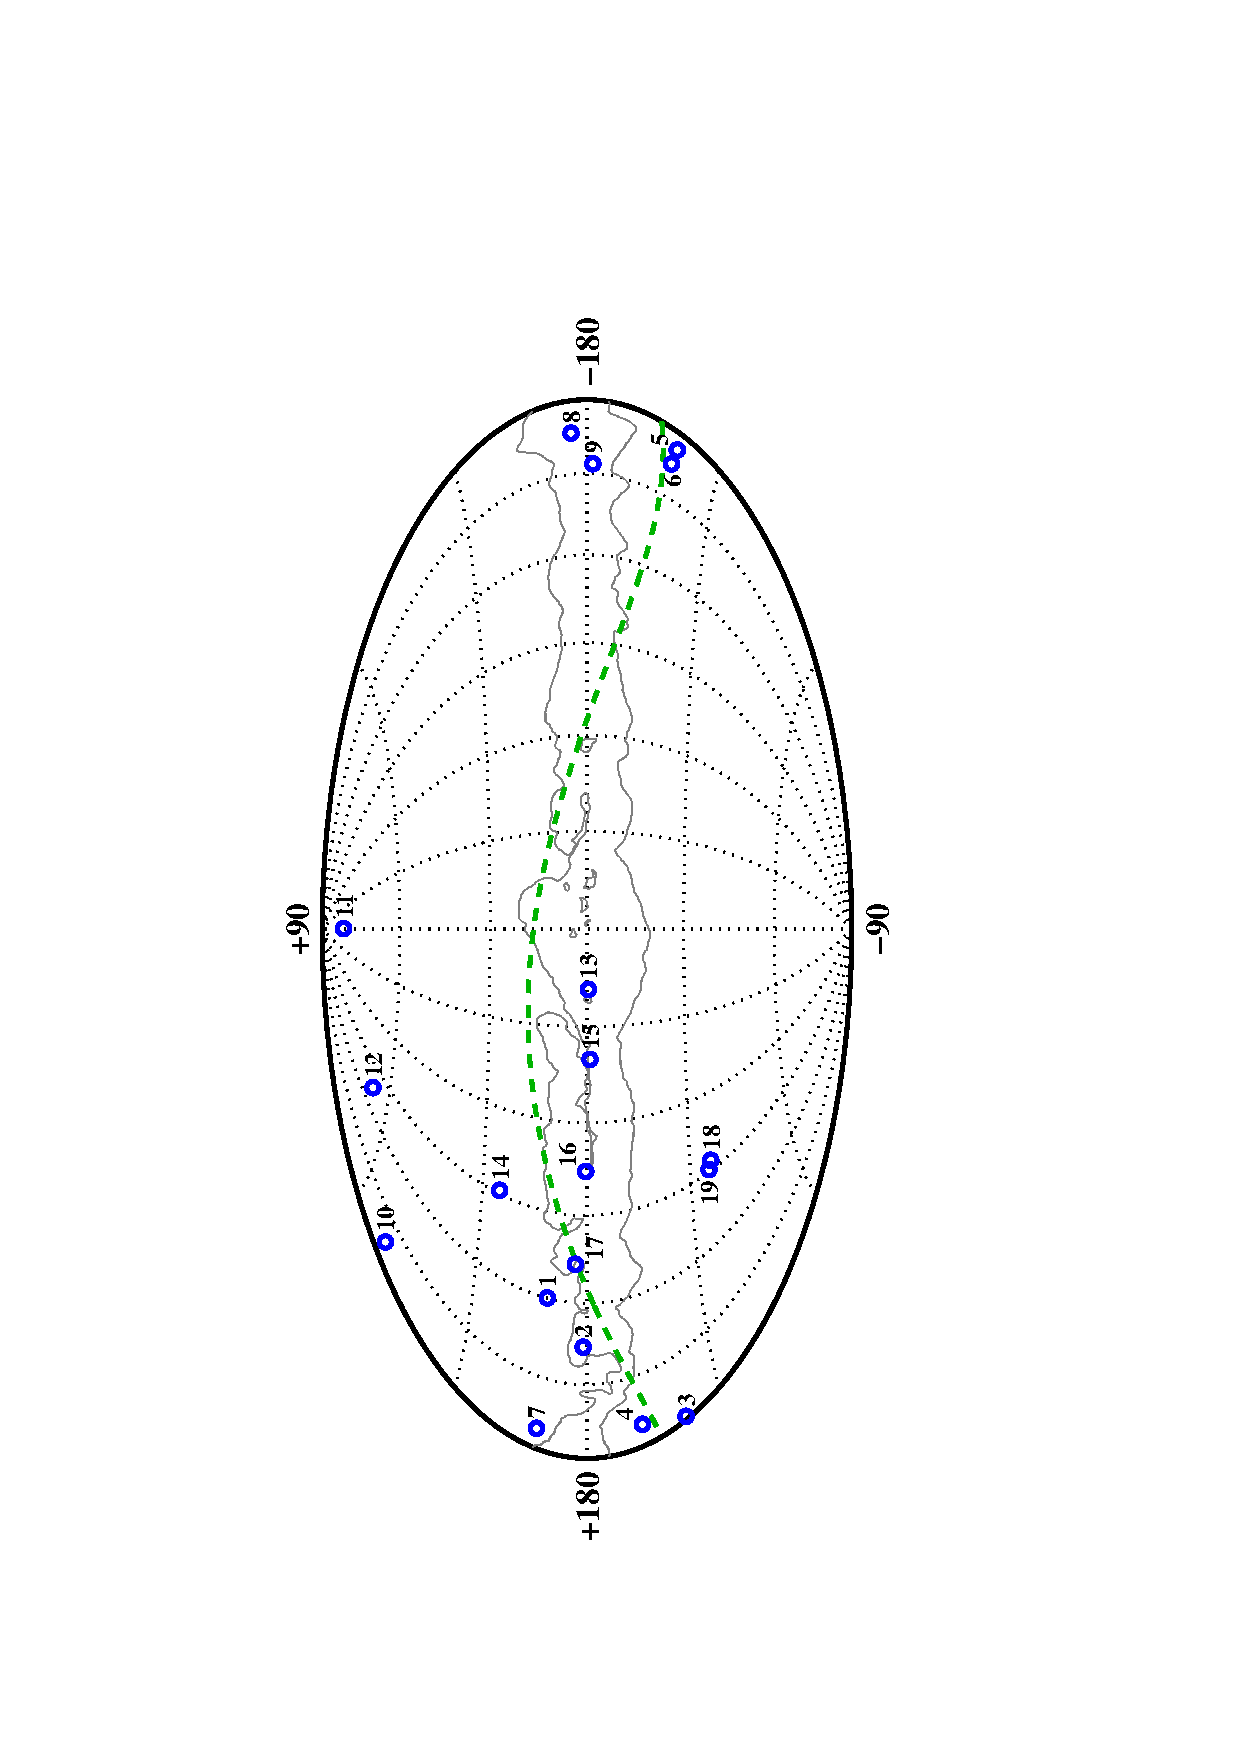
\includegraphics[angle=270,width=\textwidth]{plots/chap-observations/sources.pdf}
\caption{\label{FIG::OBSERVATIONS::SOURCES} The 19 unidentified EGRET
sources considered in this survey, plotted in Galactic coordinates. The
Milky Way and Gould Belt are also depicted, as described in 
chapter~\ref{CHAP::INTRODUCTION}. The candidate sources are labeled
by their positions in table~\ref{TAB::OBSERVATIONS::CATALOGDATA}.}
\end{figure}

\begin{table}[p]
\caption{\label{TAB::OBSERVATIONS::CATALOGDATA} Summary of the 3EG and 
GeV catalog entries for the 19 unidentified sources observed in the
survey.}
\centerline{\rotatebox{90}{\begin{minipage}{0.94\textheight}
\begin{tabular}{llllllllll}\hline
& Source Name & \multicolumn{2}{l}{Coordinates$^1$} &
\multicolumn{3}{l}{Third EGRET Catalog} &
\multicolumn{2}{l}{GeV Catalog} & Var. \\
& & & & Error$^2$ &
\multicolumn{2}{l}{Spectrum$^{3a}$} & Error & 
Flux$^{3b}$  & Indx.$^4$ \\
& & $b$ & $l$ & $\theta_{95}$ [$deg$] & $F\pm\Delta F$ & $\Gamma\pm\Delta\Gamma$ & 
$\theta_{95}$ [$deg$] & $F\pm\Delta F$ & $\delta$ \\\hline
1  & 3EG~J0010$+$7309 &  $10.56$ & $119.87$ & 0.25$\times$0.22 &  42.3$\pm$5.5 & 1.85$\pm$0.10 & 0.43             &  5.8$\pm$1.2 & 0.26 \\
2  & 3EG~J0241$+$6103 &   $0.99$ & $135.85$ & 0.21$\times$0.15 &  69.3$\pm$6.1 & 2.21$\pm$0.07 & 0.31             &  6.9$\pm$1.3 & 0.38 \\
3  & 3EG~J0423$+$1707 & $-22.21$ & $178.68$ & 0.88$\times$0.65 &  15.8$\pm$2.7 & 2.43$\pm$0.21 & -                &  -           & 0.42 \\
4  & GeV~J0433$+$2907 & $-12.58$ & $170.50$ & 0.19$\times$0.16 &  22.0$\pm$2.8 & 1.90$\pm$0.10 & 0.35             &  3.3$\pm$0.7 & 0.40 \\
5  & 3EG~J0450$+$1105 & $-20.55$ & $187.89$ & 0.65$\times$0.61 &  14.9$\pm$2.5 & 2.27$\pm$0.16 & -                &  -$^5$       & 1.13 \\
6  & GeV~J0508$+$0540 & $-19.81$ & $195.32$ & -                &  -            & -             & 0.62             &  1.4$\pm$0.4$^6$ & -$^7$\\
7  & 3EG~J0613$+$4201 &  $11.45$ & $171.38$ & 0.66$\times$0.46 &   9.0$\pm$2.3 & 1.92$\pm$0.26 & 0.65             &  1.8$\pm$0.6$^6$ & 0.72 \\
8  & 3EG~J0628$+$1847 &   $3.64$ & $193.60$ & 0.66$\times$0.49 &  23.9$\pm$4.0 & 2.30$\pm$0.10 & -                &  -           & -$^8$ \\
9  & 3EG~J0634$+$0521 &  $-1.22$ & $206.15$ & 0.85$\times$0.50 &  15.0$\pm$3.5 & 2.03$\pm$0.26 & -                &  -$^5$       & $<$0.88 \\
10 & 3EG~J1009$+$4855 &  $52.15$ & $166.93$ & 1.12$\times$0.80 &   4.8$\pm$1.4 & 1.90$\pm$0.37 & -                &  -           & $<$0.94 \\
11 & 3EG~J1323$+$2200 &  $81.15$ & $359.63$ & 0.52$\times$0.43 &   5.2$\pm$1.6 & 1.86$\pm$0.35 & -                &  -$^5$       & 1.09 \\
12 & 3EG~J1337$+$5029 &  $65.06$ & $105.18$ & 0.77$\times$0.66 &   9.2$\pm$2.6 & 1.83$\pm$0.29 & -                &  -           & 0.53 \\
13 & 3EG~J1826$-$1302 &  $-0.42$ &  $18.41$ & 0.55$\times$0.39 &  46.3$\pm$7.3 & 2.00$\pm$0.11 & 0.32             &  9.9$\pm$1.7 & 0.88 \\
14 & 3EG~J1835$+$5918 &  $25.08$ &  $88.74$ & 0.16$\times$0.13 &  60.6$\pm$4.4 & 1.69$\pm$0.07 & 0.27             & 10.2$\pm$1.4 & 0.15 \\
15 & GeV~J1907$+$0557 &  $-0.88$ &  $40.08$ & -                &  -            & -             & 0.38$\times$0.28 &  9.2$\pm$1.9 & -$^7$ \\
16 & GeV~J2020$+$3658 &   $0.24$ &  $75.29$ & 0.35$\times$0.26 &  59.1$\pm$6.2 & 1.86$\pm$0.10 & 0.28$\times$0.21 & 11.2$\pm$1.5 & 0.36 \\
17 & 3EG~J2227$+$6122 &   $3.19$ & $106.55$ & 0.50$\times$0.41 &  41.3$\pm$6.1 & 2.24$\pm$0.14 & 0.54             &  3.9$\pm$1.2$^6$ & 0.20 \\
18 & 3EG~J2248$+$1745 & $-36.15$ &  $86.00$ & 1.14$\times$0.78 &  12.9$\pm$3.5 & 2.11$\pm$0.39 & -                &  -           & 0.65 \\
19 & 3EG~J2255$+$1943 & $-34.35$ &  $89.85$ & 2.67$\times$2.33 &   5.8$\pm$2.8 & 2.36$\pm$0.61 & -                &  -           & 1.18 \\\hline
\end{tabular}\\[1.2ex]
\centerline{\footnotesize{\begin{tabular}{rp{0.9\textwidth}}
$^1$ & Galactic coordinates from the 3EG or GeV catalog as 
appropriate.\\
$^2$ & Elliptical fits to 95\% error contours for 3EG sources 
from \citet{REF::MATTOX::APJS2001}.\\
$^3$ & Flux at energies greater than (a) 100\,MeV and (b) 
1\,GeV in units of $10^{-8}$\,cm$^{-2}$s$^{-1}$.\\
$^4$ & Variability index from \citet{REF::NOLAN::APJ2003}, higher
values indicate more source variability.\\
$^5$ & Listed as source of repeating weak outbursts of GeV \Grays
\citep[Table~2 of][]{REF::MACOMB::ICRC1999}.\\
$^6$ & Listed as a low-significance source of GeV \Grays in 
table~2 or 3 of \citet{REF::LAMB::APJ1997}.\\
$^7$ & \citet{REF::NOLAN::APJ2003} present variability indices 
for 3EG sources only.\\
$^8$ & As noted in \citet{REF::NOLAN::APJ2003}, 3EG~J0628$+$1847 
failed a consistency check during the analysis. 
\end{tabular}}}
\end{minipage}}}
\end{table}

\section{Individual observations}

Details and results of the observations are presented below, with a
discussion of each candidate source and possible counterparts in the
fields of view. For each object, with the exception of GeV~J0508$+$0540,
a two dimensional analysis has been performed and a map of the excess
(or deficit) of {\Grayc}-like events produced. For objects where a
significant excess of events is detected, a map of the significance of
the emission is presented. For those without a significant excess,
i.e.\ those which do not have an excess at a $3\sigma$ level or
higher, a map of the upper limit of VHE \Gray emission is presented,
at a 99\% confidence level. The maps are overlayed with the 3EG error
contours\footnote{The contours were extracted from the on-line version
of the catalog which contains maps of the $(TS)^{1/2}$ likelihood
statistic} at the 50\%, 69\%, 95\% and 99\% confidence level, as
described by \citet{REF::MATTOX::APJ1996}. For GeV sources, the 95\%
error ellipse is shown, based on the parameters in the catalog.  From
each of these maps, the maximum upper limit within the 3EG (or GeV)
error-box is presented, corresponding to a conservative VHE upper
limit for the HE \Gray source. For each object that has potentially
interesting counterparts at other wavelengths, such as radio and x-ray
counterparts suggested in the literature, upper limits are also
presented for emission from the location of the possible counterparts;
these limits are generally lower than the limit on emission from the
entire error-box. Finally, for the sources with an entry in the 3EG
catalog, the \Gray spectrum is shown, extrapolated to 1\,TeV, with the
VHE upper limit for the error-box overlaid.

\subsection{3EG~J0010$+$7309}

The 3EG source J0010$+$7309 has long been suggested as possibly
associated with the supernova CTA~1, G119.5$+$10.2 in
\citet{REF::GREEN::WEB2001}, on the basis of its position. The
first images of CTA~1 at x-ray energies were recorded with the ROSAT
instrument; the source has been well studied with later x-ray
instruments, such as ASCA and XMM-Newton
\citep{REF::SEWARD::APJ1995, REF::SLANE::APJ1997, REF::SLANE::APJ2004}.
The observations indicate that the x-ray emission from CTA~1 must be
described by three components; the first is a thermal, shell-type,
component associated with the Sedov expansion of the remnant into the
inter-stellar medium (ISM), which appears to be occurring in a region
of low density. The shell-type nebula is large,
$\sim107$\,arcmin in diameter, and $1.4\pm0.3$\,kpc.\ in
distance. There is a ``blow-out'' region in the north of the nebula
where the nebula has evidently expanded quickly into a region of
particularly low density. The second x-ray component is evident as
a region of bright, non-thermal emission at the center of the
nebula. This emission is consistent with synchrotron emission from a
central PWN, with a power-law spectral index of 2.3 and total x-ray
luminosity of $L_\mathrm{X}=5.6\times10^{33}$\,erg\,s$^{-1}$. Finally,
ROSAT detected a non-thermal compact point source, RX~J0007.0$+$7302,
which may be associated with a pulsar at the center of the
nebula, although no pulsations have been detected in radio or
x-rays. \citet{REF::SLANE::APJ2004} report on
XMM observations of the compact source; its spectrum is
best fit by a power-law with index of 1.5 and total luminosity of
$L_\mathrm{X}=4.7\times10^{31}$\,erg\,s$^{-1}$.

The \Gray source has a large, steady $>$100\,MeV flux, a hard spectrum
of $\Gamma=1.85$, with possible evidence of softening above 2\,GeV and
a low variability index of
$\delta=0.26$. \citet{REF::BRAZIER::MNRAS1998} suggest that the \Grays
are most likely associated with the compact source which lies within
the 95\% confidence contour of the EGRET observations.  As noted by
\citet{REF::SLANE::APJ2004}, the power-law x-ray spectrum of the
compact source can be extrapolated to \Gray energies without a
spectral break. Other compact x-ray sources in the region are
suggested as possible counterparts by
\citet{REF::SEWARD::APJ1995}; \citet{REF::BRAZIER::MNRAS1998} dismiss
all but RX~J0010$+$7309.

\begin{figure}[t]
\resizebox*{\textwidth}{!}{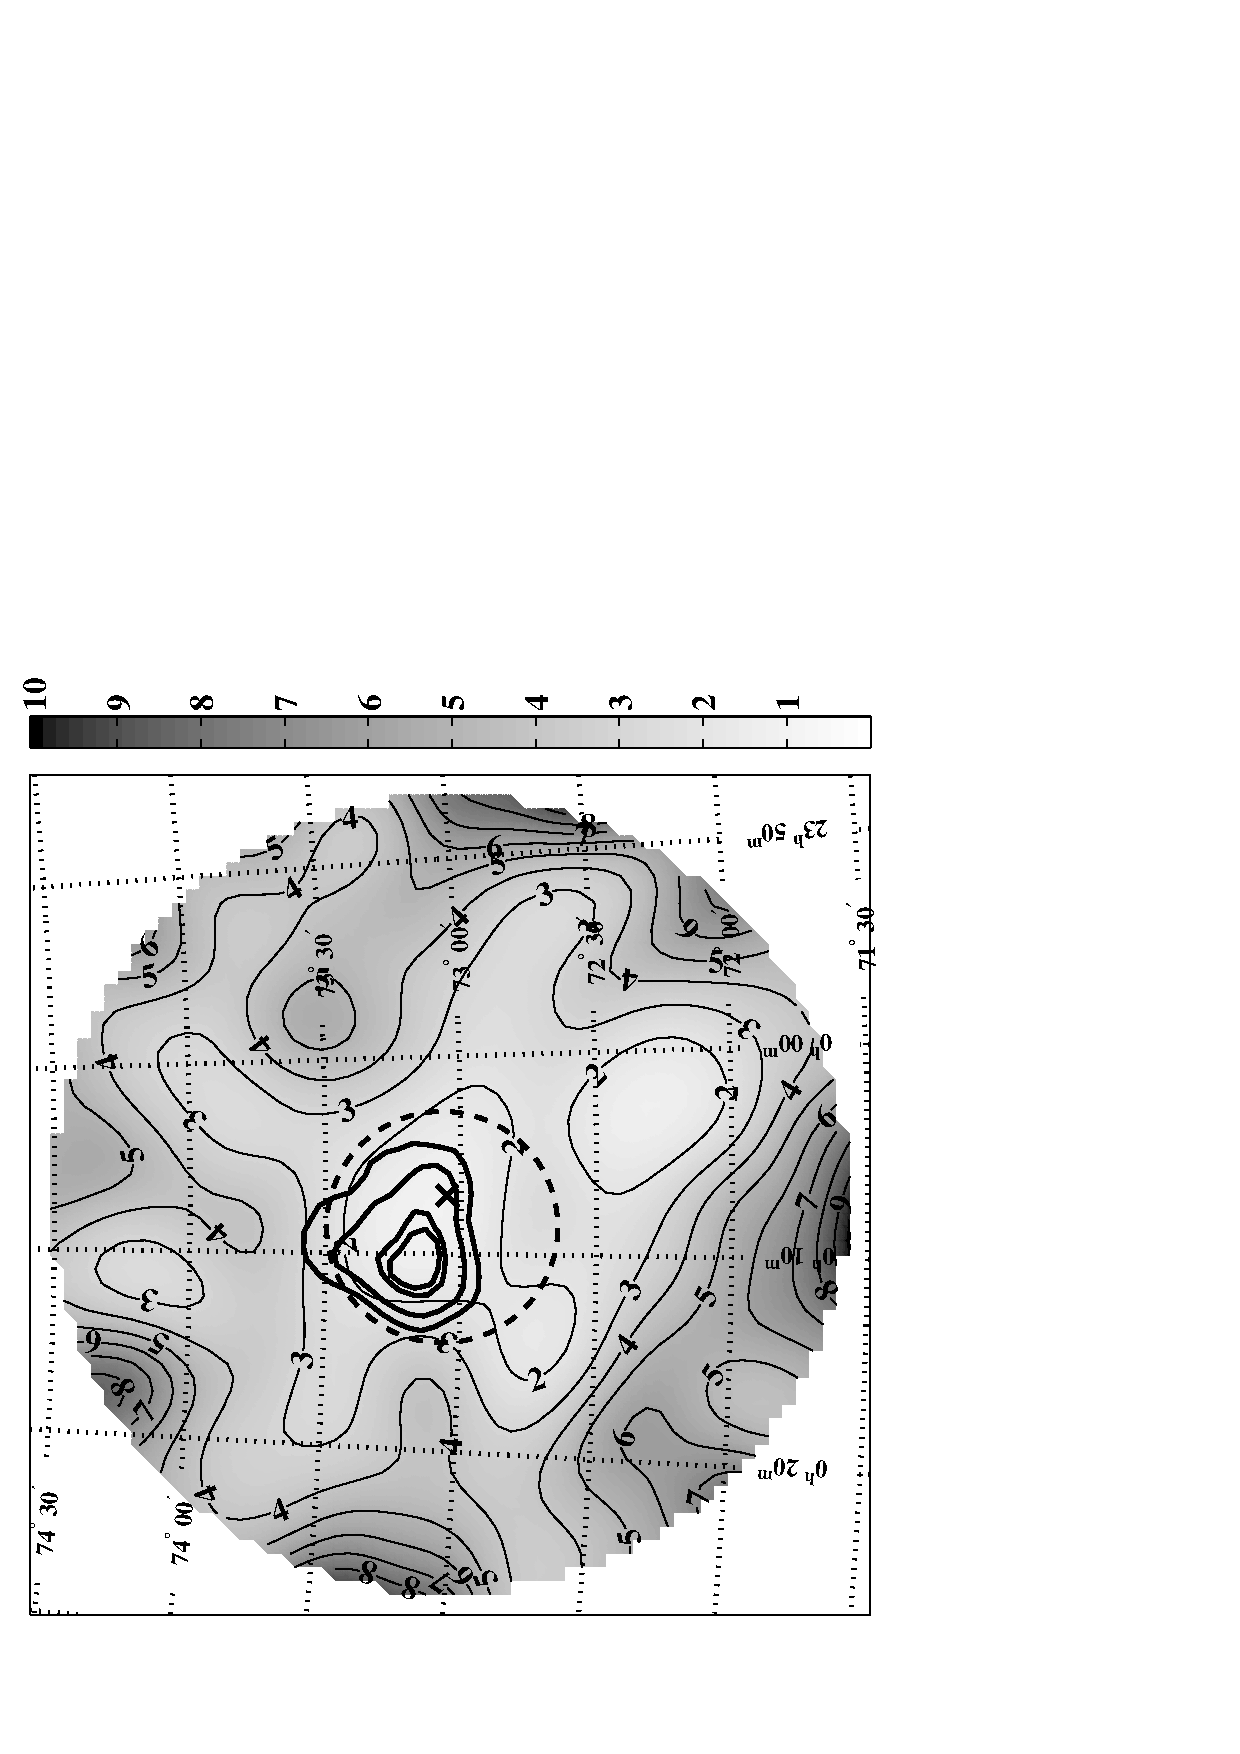
\includegraphics[draft=false,width=\textwidth,angle=270]{plots/chap-observations/loenergy/J0010+7309_sul_conv_bw.pdf}\includegraphics[width=\textwidth,angle=270]{plots/chap-observations/spectra/3EG_J0010+7309.pdf}}
\caption{\label{FIG::OBSERVATIONS::J0010} (Left) Limits on emission from 
3EG J0010$+$7309 in units of $10^{-11}$\,cm$^{-2}$\,s$^{-1}$. The 3EG
error contours are overlaid as heavy lines, the GeV catalog contour is
shown as a broken circle. (right) Spectrum from the on-line version of
the 3EG catalog with the limit at 350\,GeV.}
\end{figure}

The VHE observations reported here consist of a combined 195\,min.\
exposure on the source, pointed at the center of the nebula, offset by
0.27 degrees from the center of the 3EG source. The data were taken
during late 1999. No emission is detected at a significant level, an
upper limit on emission from anywhere within the 95\% error circle of
$F_{(>350\,\mathrm{GeV})}<2.2\times10^{-11}$\,cm$^{-2}$\,s$^{-1}$ is
calculated. Figure~\ref{FIG::OBSERVATIONS::J0010} shows the map of the
upper limit of point source emission from the region and the 3EG
power-law spectrum extrapolated to 350\,GeV, with the upper limit
superimposed. It is clear from the diagram that extrapolating the
EGRET power-law to the VHE regime is in conflict with these
observations by an order of magnitude. A cut-off in the spectrum is
required to reconcile the observations. Some evidence for this cut-off
is also visible in the highest energy bins of the EGRET spectrum. The
cut-off supports the supposition that the \Grays originate from a
pulsar. The upper limit from RX~J0007.0$+$7302, whose location is
marked with an ``X'' in figure~\ref{FIG::OBSERVATIONS::J0010}, is
$F_{(>350\,\mathrm{GeV})}<1.1\times10^{-11}$\,cm$^{-2}$\,s$^{-1}$.

\begin{table}[t]
\caption{\label{TAB::OBSERVATIONS::J0010} Upper limits for candidates
in 3EG~J0010$+$7309 field.}
\centerline{\begin{tabular}{lllll}\hline
Source Name & \multicolumn{2}{l}{Coordinates} & Extent & Upper Limit \\
& $\alpha_{2000}$ & $\delta_{2000}$ & deg & $\times10^{-11}$\,cm$^{-2}$\,s$^{-1}$\\\hline
3EG~J0010$+$7309     & $00^h09^m36.6^s$ & $+73^\circ10^{\prime}57.4^{\prime\prime}$ & 0.25$\times$0.22 & 2.2 \\
RX~J0007.0$+$7302    & $00^h07^m02.2^s$ & $+73^\circ03^{\prime}07.1^{\prime\prime}$ & -                & 1.1 \\\hline
\end{tabular}}
\end{table}

\subsection{3EG~J0241$+$6103}

First detected by the COS-B instrument, and designated as 2CG~135$+$01,
the \Gray source 3EG~J0241$+$6103 has been the subject of much study
over the past 25 years. On the basis of the COS-B position, the source
was been associated with the quasar QSO~4U0241$+$61, at redshift
$z=0.0438$, \citep{REF::MARASCHI::NATURE1978,
REF::APPARAO::NATURE1978} and with the non thermal radio source
GT~0236$+$610 \citep{REF::GREGORY_TAYLOR::NATURE1978,
REF::HERMSEN::NATURE1977}. Observations with EGRET refined the
position estimate, and eliminated the possible association with the
quasar \citep{REF::KNIFFEN::APJ1997}, which lies over a degree away.
The non-thermal radio source quickly came to be associated with the
binary system LSI~$+$61$^\circ$303 \citep{REF::GREGORY::AJ1979}, an
unusual object which has been identified at radio, optical and x-ray
energies. LSI~$+$61$^\circ$303 exhibits periodic radio outbursts at a
period of $\sim$26.5 days \citep{REF::TAYLOR_GREGORY::APJ1982}. The
outbursts do not occur at a constant phase relative to this period;
there is evidence that both the phase and amplitude of the outbursts
vary slowly with a $\sim$4.6\,yr.\ phase modulation period
\citep{REF::GREGORY::APJ1999, REF::GREGORY::APJ2002}. 
\citet{REF::PAREDES::AA1997} report a periodic modulation of the
x-ray light-curve from the ASM satellite, which appears to occur at a
constant orbital phase, corresponding to the periastron. No pulsations
have been detected in the x-ray signal, suggesting that the x-ray
emission is not directly from the neutron star companion. 
\citet{REF::MASSI::AA2001} report the existence of a one-sided jet
from the object on a milli-arcsecond scale. A number of models have
been suggested to explain the radio and x-ray emission and to account
for the possibility of \Gray
emission. \citet{REF::GREGORY_NEISH::APJ2002} provide an introduction
to the observational status of this object and provide references to
the various emission models.

\begin{figure}[t]
\resizebox*{\textwidth}{!}{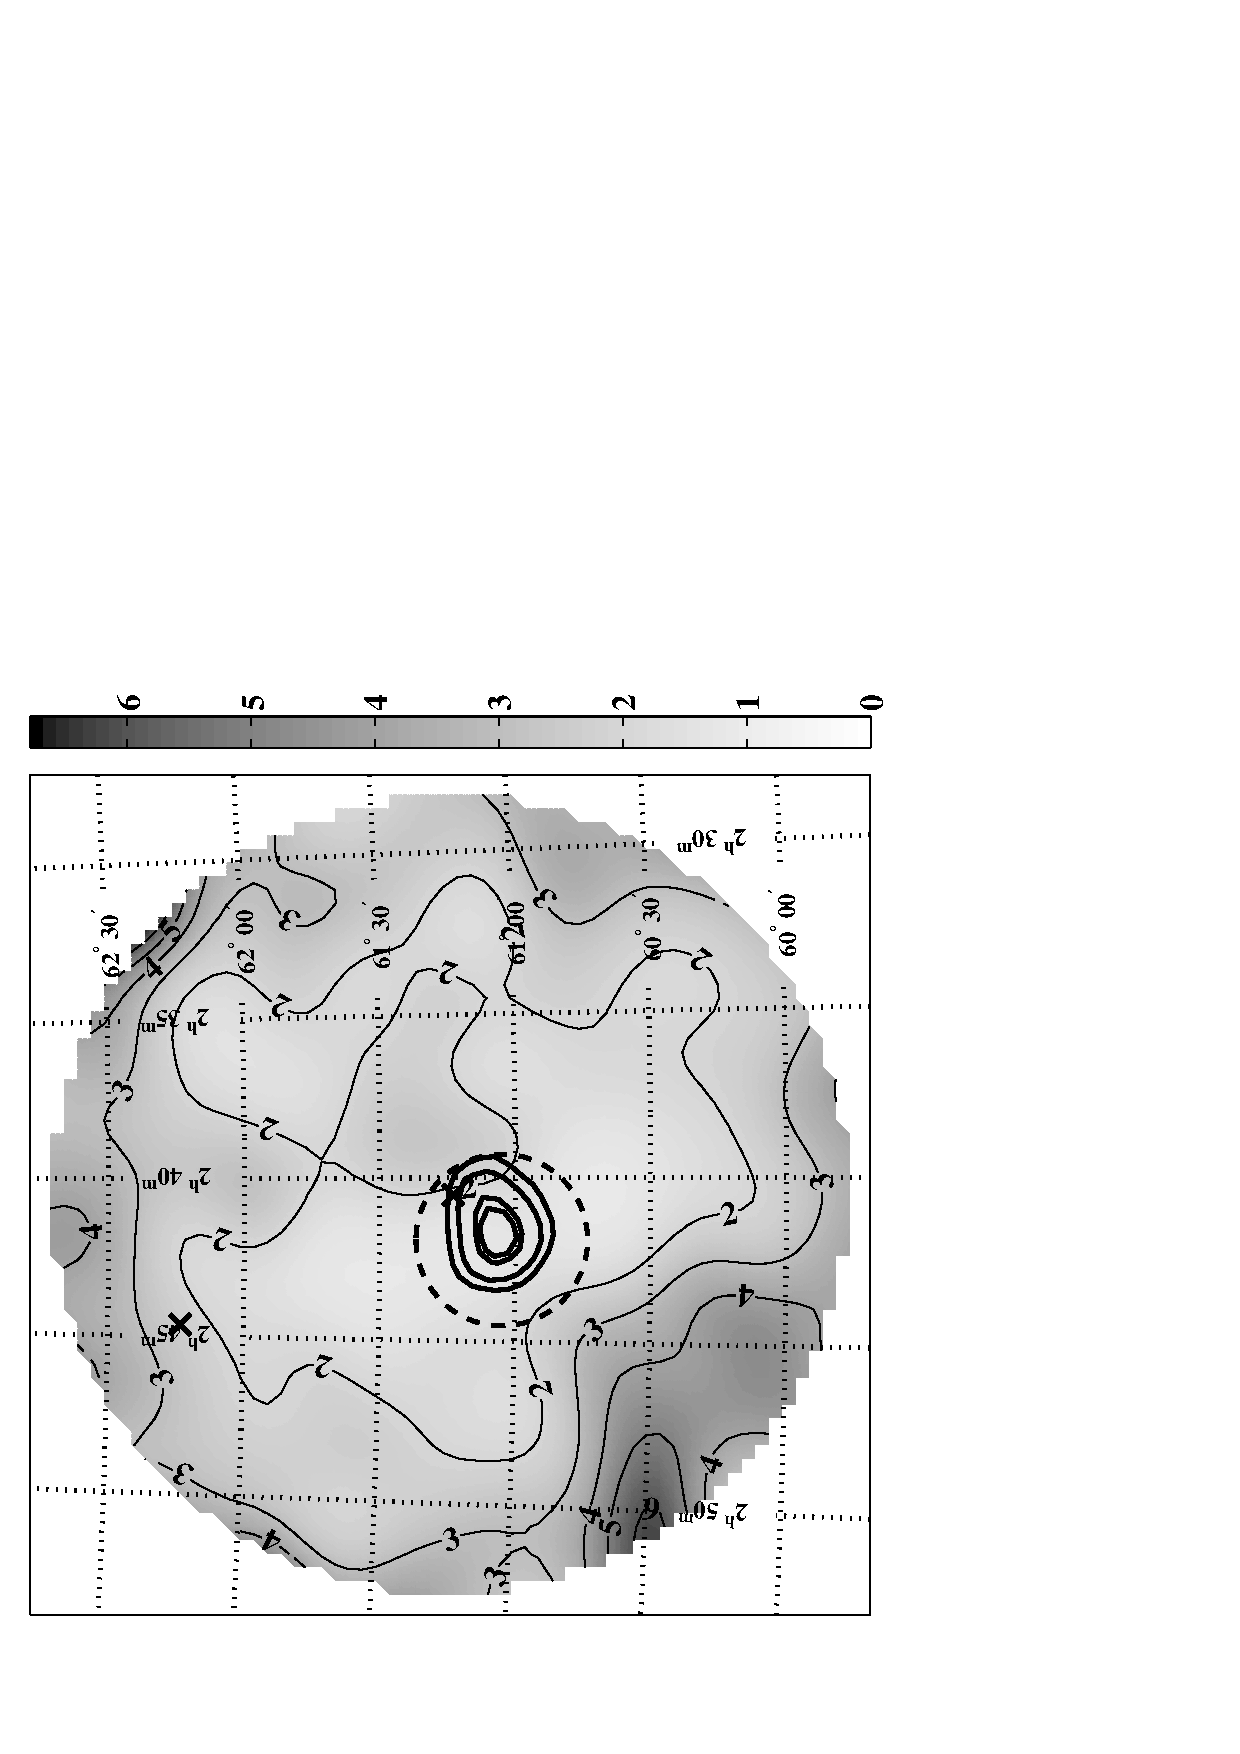
\includegraphics[draft=false,width=\textwidth,angle=270]{plots/chap-observations/loenergy/J0241+6103_sul_conv_bw.pdf}\includegraphics[width=\textwidth,angle=270]{plots/chap-observations/spectra/3EG_J0241+6103.pdf}}
\caption{\label{FIG::OBSERVATIONS::J0241} (Left) Limits on emission from 
3EG J0241$+$6103 in units of $10^{-11}$\,cm$^{-2}$\,s$^{-1}$. The 3EG
error contours are overlaid as heavy lines, the GeV catalog contour is
shown as a broken circle. (right) Spectrum from the on-line version of the 3EG
catalog with upper limit at 350\,GeV. The limit at 500\,GeV from 
\citet{REF::HALL::APJ2003} is also indicated.}
\end{figure}

The 3EG source has a spectral index of $\Gamma=2.21$, a large 100\,MeV
flux and shows evidence of variability. \citet{REF::KNIFFEN::APJ1997}
show that the variations in the \Gray flux are not correlated with the
radio outbursts. An exposure of 524\,min.\ was taken with the Whipple
telescope between November 2000 and February 2001, centered on the
binary system, offset by $\sim$0.25$^\circ$ from the center of the 3EG
source. No significant emission is detected and an upper limit of
$F_{(>350\,\mathrm{GeV})}<2.2\times10^{-11}$\,cm$^{-2}$\,s$^{-1}$ is
derived for emission withing the 3EG 95\%
contour. Figure~\ref{FIG::OBSERVATIONS::J0241} shows a map of upper
limits of emission from the region with the location of
LSI~$+$61$^\circ$303 and QSO~4U0241$+$61 indicated with an ``X'' (near
the center and displaced by a degree to the north respectively). It is
evident from the figure that the binary system lies outside of the
95\% confidence contour of the EGRET data, although it does lie within
the considerably larger 95\% confidence circle from the GeV
catalog. As noted by
\citet{REF::ROBERTS::APJS2001} based on an image of the region with
the ASCA instrument, there are no good x-ray candidates within the
95\% confidence contour for this
source. Table~\ref{TAB::OBSERVATIONS::J0241} shows the upper limits
derived for these candidate sources.

\begin{table}[t]
\caption{\label{TAB::OBSERVATIONS::J0241} Upper limits for candidates
in 3EG~J0241$+$6103 field.}
\centerline{\begin{tabular}{lllll}\hline
Source Name & \multicolumn{2}{l}{Coordinates} & Extent & Upper Limit \\
& $\alpha_{2000}$ & $\delta_{2000}$ & deg & $\times10^{-11}$\,cm$^{-2}$\,s$^{-1}$\\\hline
3EG~J0241$+$6103     & $02^h41^m31.3^s$ & $+61^\circ04^{\prime}12.3^{\prime\prime}$ & 0.21$\times$0.15 & 2.2 \\
LSI~$+$61$^\circ$303 & $02^h40^m31.4^s$ & $+61^\circ13^{\prime}45.6^{\prime\prime}$ & -                & 1.7 \\
QSO~4U0241$+$61      & $02^h44^m37.3^s$ & $+62^\circ13^{\prime}57.0^{\prime\prime}$ & -                & 2.3 \\\hline
\end{tabular}}
\end{table}

LSI~$+$61$^\circ$303 was previously observed with the Whipple
telescope between 1996 and 1999, with no significant excess of \Grays
being observed; a limit of
$F_{(>500\,\mathrm{GeV})}<0.88\times10^{-11}$\,cm$^{-2}$\,s$^{-1}$ was
reported by \citet{REF::HALL::APJ2003}. Assuming that the 3EG source
corresponds to the LSI~$+$61$^\circ$303, this paper shows that an
exponential cutoff is required in the extrapolated EGRET spectrum to
accommodate the VHE observations. Almost all of the flux phase space
at 350\,GeV allowed by extrapolating the EGRET spectrum is ruled out
by the upper limit reported here. After a quarter century of study,
2CG~135$+$01 remains one of the most puzzling of all \Gray
sources.

\subsection{3EG~J0423$+$1707}

3EG~J0423$+$1707 is an EGRET source about which very little is known at
other wavelengths. The 3EG error circle is large, at
$0.88^\circ\times0.65^\circ$, and it has the softest spectrum among
all of the sources chosen for this
survey. \citet{REF::MATTOX::APJS2001} suggest the radio source
B0422$+$1749 as a possible, but unlikely, counterpart, with a
probability of $2\times10^{-4}$.

\begin{figure}[t]
\resizebox*{\textwidth}{!}{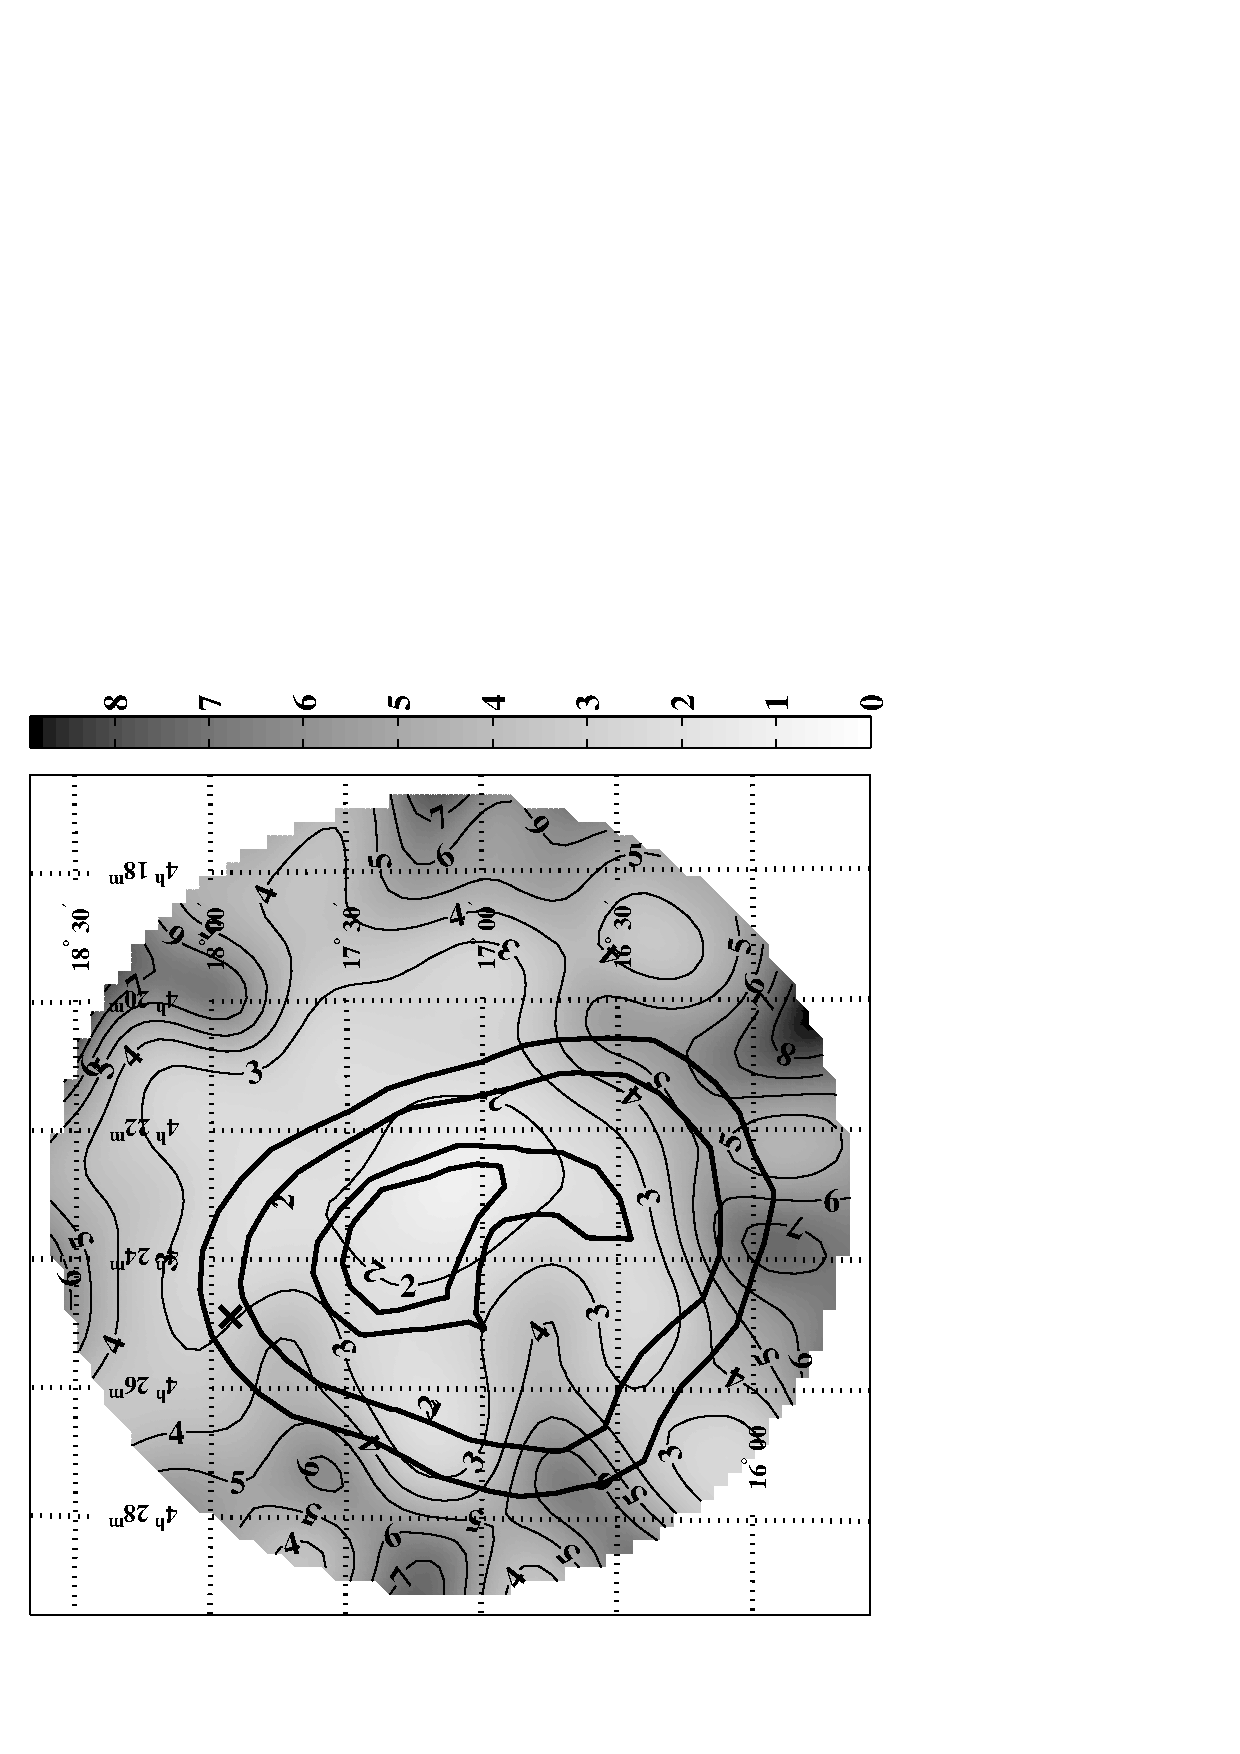
\includegraphics[draft=false,width=\textwidth,angle=270]{plots/chap-observations/loenergy/J0423+1707_sul_conv_bw.pdf}\includegraphics[width=\textwidth,angle=270]{plots/chap-observations/spectra/3EG_J0423+1707.pdf}}
\caption{\label{FIG::OBSERVATIONS::J0423} (Left) Limits on emission from 
3EG J0423$+$1707 in units of $10^{-11}$\,cm$^{-2}$\,s$^{-1}$. The 3EG
error contours are overlaid as heavy lines. (Right) Spectrum from the
on-line version of 3EG catalog with the upper limit at 350\,GeV.}
\end{figure}

\begin{table}[t]
\caption{\label{TAB::OBSERVATIONS::J0423} Upper limits for candidates
in 3EG~J0423$+$1707 field.}
\centerline{\begin{tabular}{lllll}\hline
Source Name & \multicolumn{2}{l}{Coordinates} & Extent & Upper Limit \\
& $\alpha_{2000}$ & $\delta_{2000}$ & deg & $\times10^{-11}$\,cm$^{-2}$\,s$^{-1}$\\\hline
3EG~J0423$+$1707     & $04^h23^m56.5^s$ & $+16^\circ56^{\prime}27.4^{\prime\prime}$ & 0.88$\times$0.65 & 6.6 \\
B0422$+$1749         & $04^h24^m53.4^s$ & $+17^\circ55^{\prime}49.9^{\prime\prime}$ & -                & 2.8 \\\hline
\end{tabular}}
\end{table}

The VHE observation consists of 193\,min.\ of data pointed at the center
of the 3EG source. No significant emission is observed, and an upper
limit of $F_{(>350\,\mathrm{GeV})}<6.6\times10^{-11}$\,cm$^{-2}$\,s$^{-1}$ is
derived for VHE emission within the 95\% confidence contour. A limit
of $F_{(>350\,\mathrm{GeV})}<2.8\times10^{-11}$\,cm$^{-2}$\,s$^{-1}$ applies to
the radio source B0422$+$1749. As is clear from
figure~\ref{FIG::OBSERVATIONS::J0423}, this limit does not constrain
the extrapolated EGRET spectrum.


\subsection{GeV~J0433$+$2907}

The \Gray source 3EG~J0433$+$2908 is listed as possibly being
associated with the radio source 87GB~0430$+$2859 in the 3EG catalog,
and was assumed to be an AGN. The \Gray source is unusual for an EGRET
AGN; the spectrum is particularly hard with no indication of a break
at energies up to 10\,GeV. \citet{REF::DINGUS::GAMMA2001}, analyzed
all of the EGRET photons at energies above 10\,GeV and show that three
are consistent with having originated from the location of the radio
source. At these energies the EGRET point-spread function is
considerably better than at 100\,MeV; given this improved PSF, they
calculate a probability of $1.9\times10^{-6}$ that three photons could
be associated with the source location purely by chance.
\citet{REF::WALLACE::GAMMA2001} gather together  compelling evidence 
that the radio source corresponds to an AGN: optical observations show
a featureless optical spectrum typical of a BL~Lac and the spectral
energy distribution\footnote{An SED, or $\nu F_\nu$ plot, for an
object is a graphical representation of the power an instrument would
receive across the spectrum given the assumption that its bandwidth is
proportional to the frequency. SEDs are usually displayed in units of
Ja\,Hz, W\,m$^{-2}$ or erg\,cm$^{-2}$\,s$^{-1}$ and are equivalent to
the E$^2$\,dF/dE plots presented in this chapter.}, or SED, shows a
clear two-peaked distribution, indicating synchrotron/inverse-Compton
(IC) emission that is typical for AGN. Assuming that the \Gray source
corresponds to the radio/x-ray source, the SED for 3EG~J0433$+$2908 is
shown in figure~\ref{FIG::OBSERVATIONS::SED0433}, and will be
discussed further below. No successful redshift measurements have been
made for this object, \citet{REF::HALPERN::AJ2003} report on repeated
attempts to determine the redshift and argue that $z>0.3$ for this object.

\begin{figure}[p]
\resizebox*{\textwidth}{!}{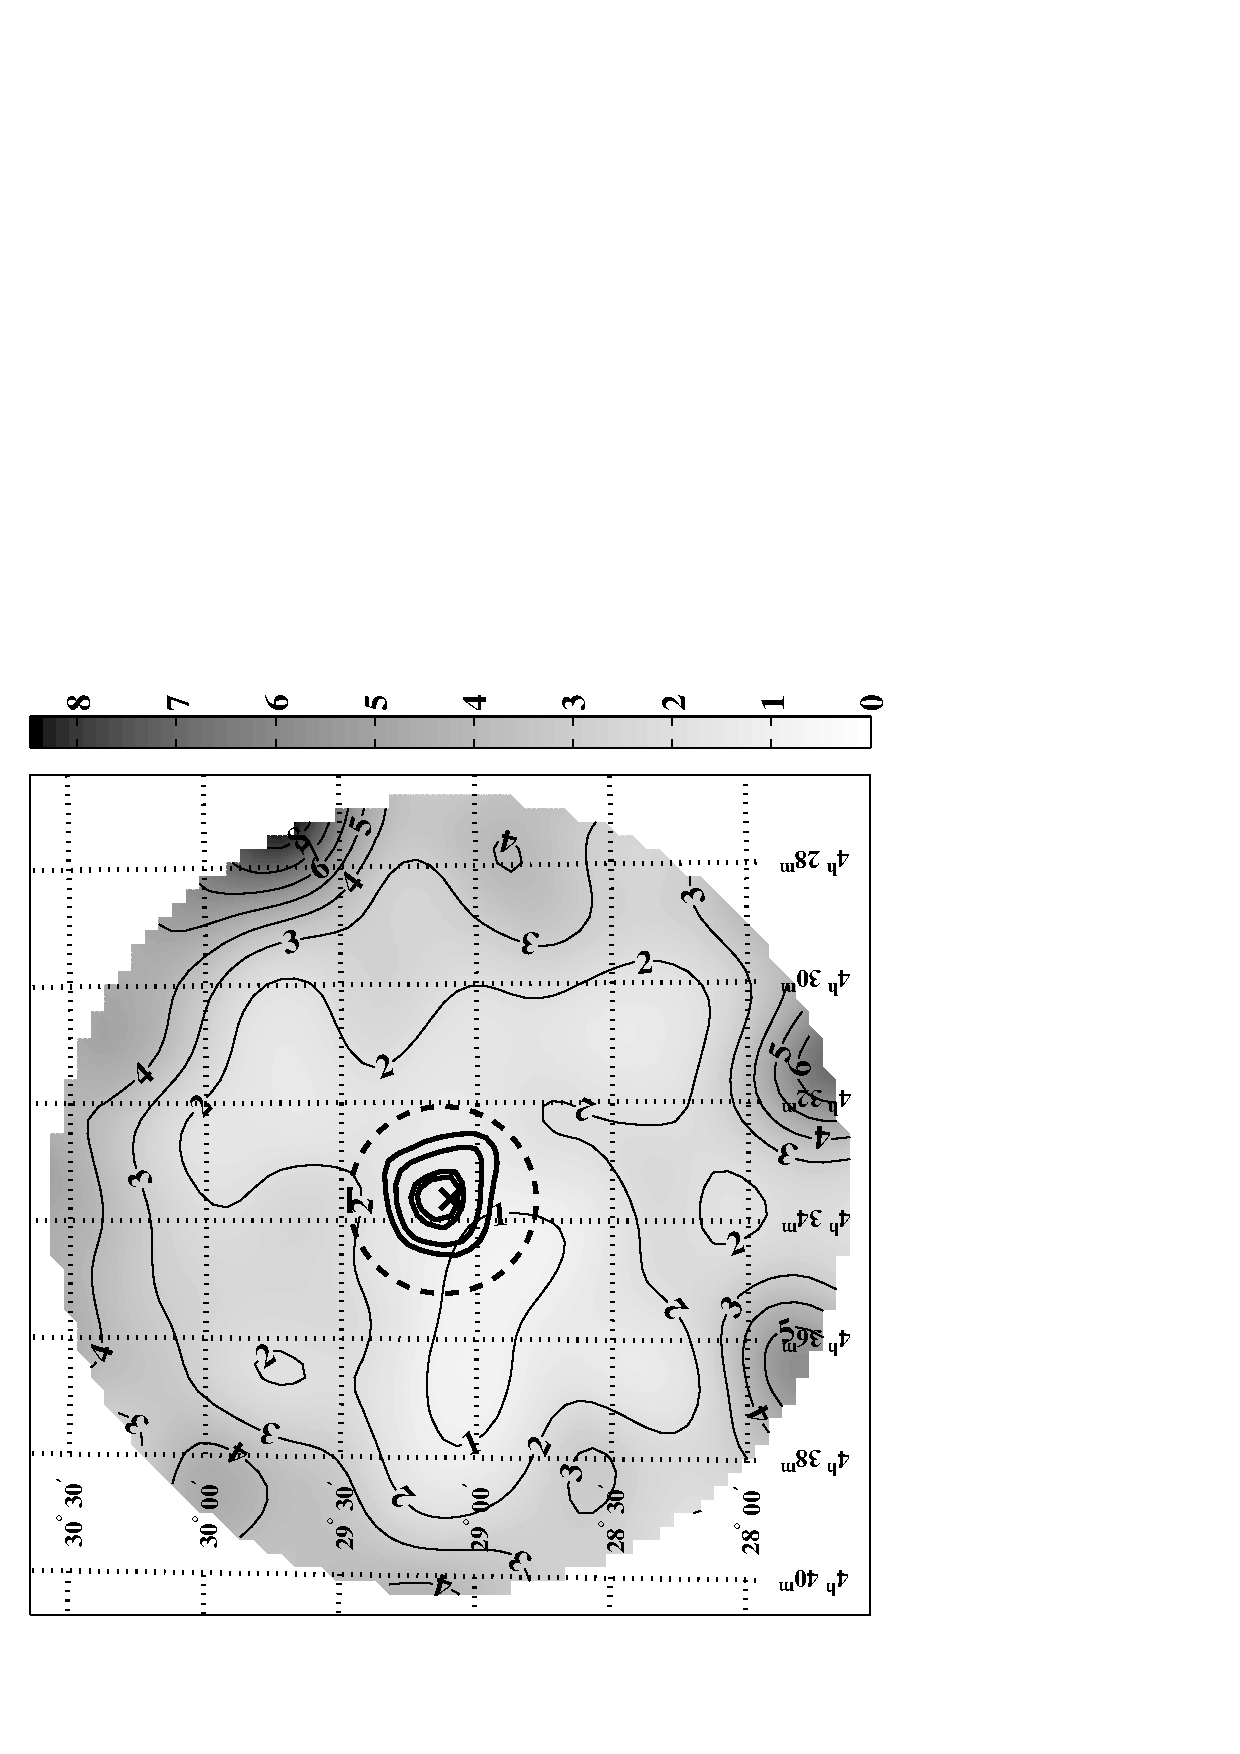
\includegraphics[draft=false,width=\textwidth,angle=270]{plots/chap-observations/loenergy/J0433+2908_sul_conv_bw.pdf}\includegraphics[width=\textwidth,angle=270]{plots/chap-observations/spectra/3EG_J0433+2908.pdf}}
\caption{\label{FIG::OBSERVATIONS::J0433} (Left) Limits on 
emission from 3EG J0433$+$2908 in units of
$10^{-11}$\,cm$^{-2}$\,s$^{-1}$. The 3EG error contours are overlaid
as heavy lines, the GeV catalog contour is shown as a broken
circle. (Right) Spectrum from the on-line version of the 3EG catalog with
the upper limit at 350\,GeV.}
\end{figure}

Between November 1999 and January 2002 a total of 1900\,min.\ of data
were taken with the Whipple instrument pointed at the GeV catalog
source location, which is coincident with the radio/x-ray source.
Prior to the publication of \citet{REF::DINGUS::GAMMA2001}, 500\,min.\
of data were collected in the \On/\Off\ mode, suitable for analysis
using the two-dimensional reconstruction technique. No significant
emission was detected; figure~\ref{FIG::OBSERVATIONS::J0433} shows the
upper limits of emission that can be derived from these data. The
upper limit within the 3EG 95\% error contour is
$F_{(>350\,\mathrm{GeV})}<1.6\times10^{-11}$\,cm$^{-2}$\,s$^{-1}$. This
limit is displayed with the 3EG spectrum in
figure~\ref{FIG::OBSERVATIONS::J0433}. To reconcile the limit with the
increasing EGRET spectrum a cut-off in the spectrum at an energy
greater than 10\,GeV is required. The remainder of the VHE data was
taken in the \Trk\ mode, and is not suitable for 2D analysis but can
provide a more sensitive limit on emission from the radio/x-ray
source. A limit of
$F_{(>350\,\mathrm{GeV})}<0.76\times10^{-11}$\,cm$^{-2}$\,s$^{-1}$ is
derived from all of the data combined. This limit is shown on a SED
for the object in figure~\ref{FIG::OBSERVATIONS::SED0433}. It must be
noted that the distribution was produced with
\textit{non-contemporaneous} data; since the SED of an AGN can change
considerably as the sources goes from a quiescent to a flaring state,
figure~\ref{FIG::OBSERVATIONS::SED0433} should be considered as
approximate. The double peaked structure is clearly visible, with the
peak in the synchrotron emission occurring somewhere in the optical to
x-ray band and the peak in the IC emission occurring between the HE
and VHE \Gray regimes.

\begin{table}[t]
\caption{\label{TAB::OBSERVATIONS::J0433} Upper limits for candidates
in 3EG~J0433$+$2908 field.}
\centerline{\begin{tabular}{lllll}\hline
Source Name & \multicolumn{2}{l}{Coordinates} & Extent & Upper Limit \\
& $\alpha_{2000}$ & $\delta_{2000}$ & deg & $\times10^{-11}$\,cm$^{-2}$\,s$^{-1}$\\\hline
3EG~J0433$+$2908     & $04^h33^m35.1^s$ & $+29^\circ07^{\prime}42.2^{\prime\prime}$ & 0.19$\times$0.16 & 1.6 \\
87GB~0430$+$2859     & $04^h33^m37.5^s$ & $+29^\circ05^{\prime}53.0^{\prime\prime}$ & -                & 0.8 \\\hline
\end{tabular}}
\end{table}

\begin{figure}[p]
\centerline{\includegraphics[angle=270,width=0.8\textwidth]{plots/chap-observations/sed0433.pdf}}
\caption{\label{FIG::OBSERVATIONS::SED0433} Spectral energy 
distribution for the radio/x-ray source RX~J0433.5$+$2906. The radio data
come from the NASA/IPAC extragalactic database (NED). The IR
observations are from the 2 micron all sky survey (2MASS). Optical
data are from \citet{REF::HALPERN::AJ2003}. The x-ray flux is from the
ROSAT all sky survey bright source catalog (RASS-BSC). Finally, the 
differential \Gray flux is from the on-line 3EG catalog.}
\end{figure}

\enlargethispage{12pt} Typically, for a low-frequency peaked BL~Lac 
(LBL) the peak in the synchrotron emission occurs in the far-infrared
to optical bands, with the IC peak below 100\,MeV, so that the
emission is falling through the EGRET energy range. Conversely, for an
HBL (high frequency peaked BL~Lac) the peak in the synchrotron
emission occurs at UV to soft x-ray energies. The IC component then
peaks at GeV to TeV energies. The SED for this object resembles most
that of an HBL. The object seems to be intermediate between the
typical EGRET BL~Lac and the VHE selected extreme HBLs. It is
reasonable to conclude that a cutoff is required between 10\,GeV and
$\sim100$\,GeV, either due to a feature intrinsic to the source
spectrum or due to absorption of the \Gray signal in the
extra-galactic background light, especially if the object is at a
distance of $z>0.3$. On the other hand, it is also possible that the
state of the object was different when the various observations were
made, i.e.\ flaring when EGRET observed it and quiescent during the
VHE observations, in which case a cutoff may not be required. However,
since the EGRET spectrum represents a mean spectrum over all viewing
periods, this is unlikely.

\subsection{3EG~J0450$+$1105}

With a spectral index of 2.27, 3EG~J0450$+$1105 has one of the softer
spectra of the sources chosen in this survey. The source is not
detected as a significant source in the GeV catalog, although it is
listed as a ``source of GeV gamma rays based upon the search for
repeating, weak outbursts'' in the second part of the catalog
\citep{REF::MACOMB::ICRC1999}. The source is consistent with being 
highly variable: it has a variability index of 1.13 and its flux is
listed in the 3EG catalog as having a maximum of
$109.5\times10^{-8}$\,cm$^{-2}$\,s$^{-1}$ during EGRET viewing period
\#36 while its average flux over all viewing periods is
$14.9\times10^{-8}$\,cm$^{-2}$\,s$^{-1}$.

\citet{REF::MATTOX::APJS2001} suggest that the \Gray source is
associated with the radio source B0446$+$1116, an AGN, with a
probability level of 0.14. \citet{REF::HALPERN::AJ2003} confirm this
association, and present their attempts to resolve a redshift for the
object. They claim that the accepted redshift of $z=1.207$ is likely
incorrect, and that the featureless spectrum they obtained makes it
impossible to derive an unambiguous redshift. Depending on how the
minor features in the spectrum are interpreted, they suggest $z=0.74$
or $z=0.21$ as possible values, with the lower value being less
likely.

\begin{figure}[p]
\resizebox*{\textwidth}{!}{\includegraphics[draft=false,width=\textwidth,angle=270]{plots/chap-observations/loenergy/J0450+1105_sul_conv_bw.pdf}\includegraphics[width=\textwidth,angle=270]{plots/chap-observations/spectra/3EG_J0450+1105.pdf}}
\caption{\label{FIG::OBSERVATIONS::J0450} (Left) Limits on 
emission from 3EG~J0450$+$1105 in units of
$10^{-11}$\,cm$^{-2}$\,s$^{-1}$. The 3EG error contours are overlaid
as heavy lines. (Right) Spectrum from the on-line version of the 3EG
catalog with the limit at 350\,GeV.}
\end{figure}

\begin{figure}[p]
\centerline{\includegraphics[angle=270,width=0.8\textwidth]{plots/chap-observations/sed0450.pdf}}
\caption{\label{FIG::OBSERVATIONS::SED0450} Spectral energy 
distribution for the radio/x-ray source PKS~B0446$+$112. The data are from
the same sources as in figure~\ref{FIG::OBSERVATIONS::SED0433}.  The
x-ray source (1RXS~J044903.0$+$112120) was not strong enough to be
included in the the RASS-BSC, the x-ray flux was estimated from the
count rate in the RASS catalog, and should be considered as
approximate.}
\end{figure}

A total of 264\,min.\ of VHE observations were made between November
2000 and February 2001. No significant excess was seen, although there
was a $3\sigma$ deficit of events at one location. Given the large
number of fields viewed in this survey, a $3\sigma$ deficit (or
excess) is not statistically significant, see
figure~\ref{FIG::ANALYSIS::SIGMASIGMA}.  The upper limits derived from
the observations are shown in figure~\ref{FIG::OBSERVATIONS::J0450}
and summarized in table~\ref{TAB::OBSERVATIONS::J0450}. The limit for
emission within the large EGRET error-box is
$F_{(>350\,\mathrm{GeV})}<5.0\times10^{-11}$\,cm$^{-2}$\,s$^{-1}$.

Figure~\ref{FIG::OBSERVATIONS::SED0450} shows an SED for the radio
source obtained from published data. The source was only weakly
detected by ROSAT, it is absent from the ROSAT bright source catalog
(RASS-BSC) but is present in the electronic version of the ROSAT all
sky survey (RASS). The SED clearly shows the two peaked structure,
typical of an LBL, with the synchrotron emission peaking in the
IR-optical band and the IC component peaking below 100\,MeV. The upper
limit derived for the location of the radio source is also shown; it
is clear from the figure that, due to the soft spectrum, the VHE upper
limit does not constrain the emission significantly.

\begin{table}[t]
\caption{\label{TAB::OBSERVATIONS::J0450} Upper limits for candidates
in 3EG~J0450$+$1105 field.}
\centerline{\begin{tabular}{lllll}\hline
Source Name & \multicolumn{2}{l}{Coordinates} & Extent & Upper Limit \\
& $\alpha_{2000}$ & $\delta_{2000}$ & deg & $\times10^{-11}$\,cm$^{-2}$\,s$^{-1}$\\\hline
3EG~J0450$+$1105  & $22^h15^m06.5^s$ & $+31^\circ28^{\prime}55.7^{\prime\prime}$ & 0.65$\times$0.61 & 5.0 \\
B0446$+$1116      & $04^h49^m07.7^s$ & $+11^\circ21^{\prime}28.6^{\prime\prime}$ & -                & 1.3 \\\hline
\end{tabular}}
\end{table}

\subsection{GeV~J0508$+$0540}

The \Gray source GeV~J0508$+$0540 is listed in the GeV catalog as a
``low-significance source'', with $23\pm7$ photons detected from the
source at E$>$1\,GeV. It was not seen significantly at 100\,MeV, and
consequently had no corresponding 3EG
entry. \citet{REF::DINGUS::GAMMA2001} list two EGRET photons with
energies greater than 40\,GeV from the object. The two photons are
consistent with having originated from the BL~Lac 0509$+$056, to
within 4\,arcmin, with probability of $1.3\times10^{-8}$ of occurring
by chance. \citet{REF::HALPERN::AJ2003} report several unsuccessful
attempts to measure the redshift of this object; the optical spectra
they recorded were featureless and no host galaxy could be resolved.

The VHE observations of this source consist of 842\,min.\ of data
taken between October and December 2001, pointing at the radio/x-ray
source. The data were recorded in the \Trk\ mode, under the assumption
that the \Gray source was the AGN, and are unsuitable for analysis
with the two-dimensional method. For this source alone, no source maps
are presented. No significant excess was observed, the limit on
emission from the AGN is
$F_{(>350\,\mathrm{GeV})}<0.73\times10^{-11}$\,cm$^{-2}$\,s$^{-1}$.

An approximate SED for this object is presented in figure
\ref{FIG::OBSERVATIONS::SED0508}. Since no 3EG detection was achieved, a
differential spectrum is not available for this source; an upper limit
at 100\,MeV and the integral flux from the GeV catalog, transformed
into a differential flux assuming a differential power-law spectrum of
index 2.0\footnote{The spectrum is probably harder than 2.0 so the
fluxes may be a little \textit{higher} than plotted.}, are
displayed. No flux at $>$10\,GeV is listed in
\citet{REF::DINGUS::GAMMA2001}, due to the small number of photons
detected and a lack of understanding of the performance of
anti-coincidence shield at these energies. A preliminary flux was
obtained from the author
\citep{REF::DINGUS::PRIVATE2001} and is plotted in
figure~\ref{FIG::OBSERVATIONS::SED0508}.

\begin{figure}[t]
\centerline{\includegraphics[angle=270,width=0.8\textwidth]{plots/chap-observations/sed0508.pdf}}
\caption{\label{FIG::OBSERVATIONS::SED0508} Spectral energy 
distribution for the radio/x-ray source RX~J0509.3$+$0541. The data
come from the same sources as in
figure~\ref{FIG::OBSERVATIONS::SED0433} with the 100\,MeV upper limit
from \citet{REF::HARTMAN::APJS1999} (see
figure~\ref{FIG::INTRODUCTION::3RDEGRETUL}), the 1\,GeV \Gray flux
from \citet{REF::LAMB::APJ1997}, and the preliminary 10\,GeV point
from \citet{REF::DINGUS::PRIVATE2001}.}
\end{figure}

\begin{table}[t]
\caption{\label{TAB::OBSERVATIONS::J0508} Upper limits for RX~J0509.3$+$0541.}
\centerline{\begin{tabular}{lllll}\hline
Source Name & \multicolumn{2}{l}{Coordinates} & Extent & Upper Limit \\
& $\alpha_{2000}$ & $\delta_{2000}$ & deg & $\times10^{-11}$\,cm$^{-2}$\,s$^{-1}$\\\hline
RX~J0509.3$+$0541        & $05^h09^m26.0^s$ & $+05^\circ41^{\prime}35.4^{\prime\prime}$ & - & 0.73 \\\hline
\end{tabular}}
\end{table}

EGRET did not resolve the peak in the high energy component of the
emission below 10\,GeV, suggesting that the object resembles an HBL.
There is insufficient data at lower energies to resolve the peak in
the low energy component; it is possible that the synchrotron emission
peaks at or below the IR/optical points in the SED, in which case the
x-ray emission results from IC up-scattering. Alternatively, the low
energy emission may peak between the optical and x-ray energies with
the x-rays resulting from synchrotron emission. Although it is not
possible to definitely rule out either scenario, usual SSC models
would have difficulty in explaining the \Gray emission (both lack of
100\,MeV emission and increasing emission through 10\,GeV) in the
former case. It was the fact that, like many VHE selected HBLs, the
source was not seen in the 3EG catalog that initially suggested that
this source would be an interesting one to study in the VHE
regime. Based on the preliminary 10\,GeV point, a strong cutoff in the
emission is required to accommodate the VHE upper limit. The cutoff
may be from absorption in the extragalactic background light if the
source is at a large redshift, or may be intrinsic to the source
spectrum.

\subsection{3EG~J0613$+$4201}

3EG~J0613$+$4201 is a 100\,MeV and 1\,GeV \Gray source at mid-Galactic
latitude with a relatively hard spectrum, weak flux, large error-box
and a high variability index. \citet{REF::MATTOX::APJS2001} list three
possible radio counterparts for the source, all outside of the 95\%
3EG contour. None of the potential associations are very compelling,
in each case the probability of the association being correct is
listed as $\le10^{-4}$.

\begin{table}[b]
\caption{\label{TAB::OBSERVATIONS::J0613} Upper limits for candidates
in 3EG~J0613$+$4201 field.}
\centerline{\begin{tabular}{lllll}\hline
Source Name & \multicolumn{2}{l}{Coordinates} & Extent & Upper Limit \\
& $\alpha_{2000}$ & $\delta_{2000}$ & deg & $\times10^{-11}$\,cm$^{-2}$\,s$^{-1}$\\\hline
3EG~J0613$+$4201 & $06^h14^m20.6^s$ & $+41^\circ59^{\prime}51^{\prime\prime}$ & 0.66$\times$0.46 & 4.3 \\
87GB~0609$+$4123 & $06^h12^m51.2^s$ & $+41^\circ22^{\prime}37^{\prime\prime}$ & -                & 1.9 \\
87GB~0612$+$4131 & $06^h16^m22.4^s$ & $+41^\circ30^{\prime}48^{\prime\prime}$ & -                & 3.1 \\
87GB~0614$+$4209 & $06^h18^m08.6^s$ & $+41^\circ08^{\prime}00^{\prime\prime}$ & -                & 2.9 \\\hline
\end{tabular}}
\end{table}

\begin{figure}[t]
\resizebox*{\textwidth}{!}{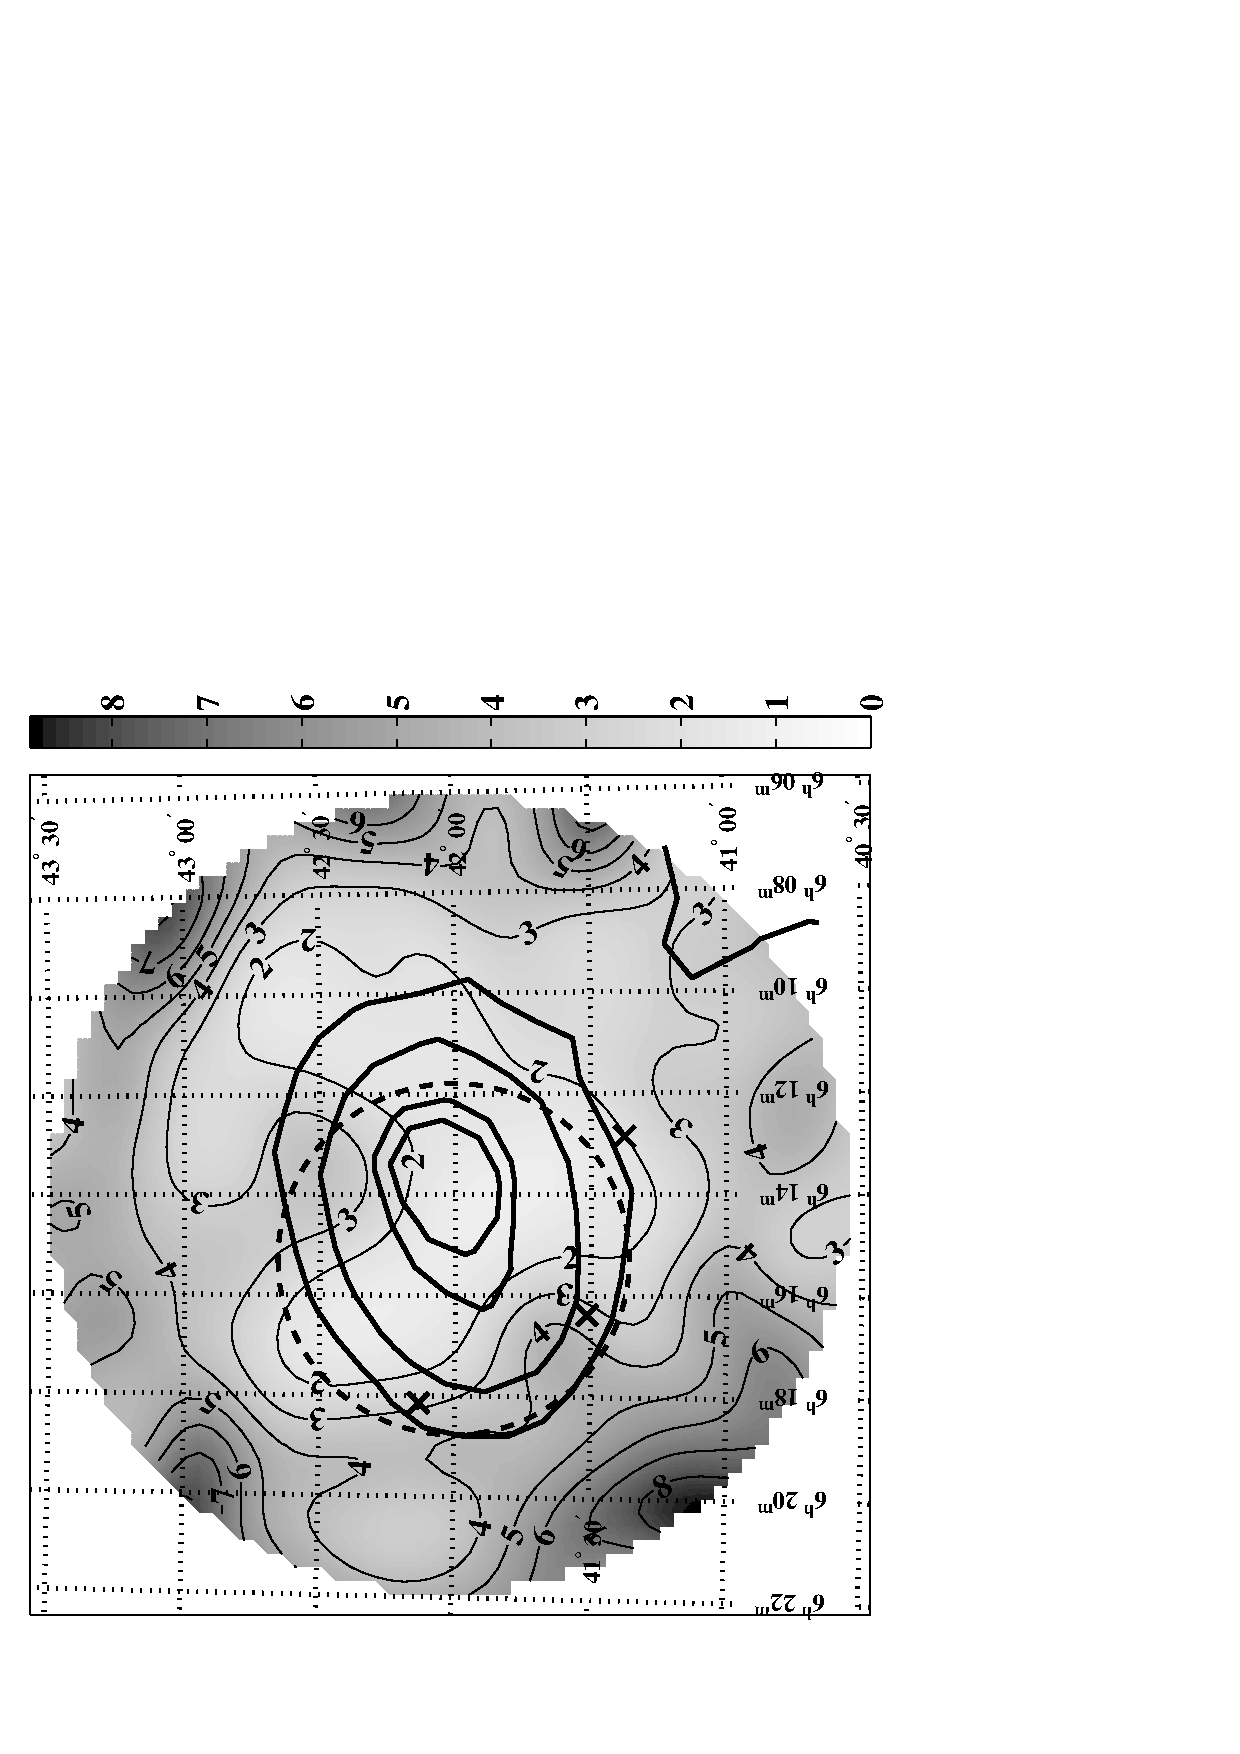
\includegraphics[draft=false,width=\textwidth,angle=270]{plots/chap-observations/loenergy/J0613+4201_sul_conv_bw.pdf}\includegraphics[width=\textwidth,angle=270]{plots/chap-observations/spectra/3EG_J0613+4201.pdf}}
\caption{\label{FIG::OBSERVATIONS::J0613} (Left) Limits on 
emission from 3EG J0613$+$4201 in units of
$10^{-11}$\,cm$^{-2}$\,s$^{-1}$. The 3EG error contours are overlaid
as heavy lines, the GeV catalog contour is shown as a broken
circle. (Right) Spectrum from the on-line version of the 3EG catalog with
the upper limit at 350\,GeV.}
\end{figure}

The VHE observations of this source, which were made over two
observing seasons, between November 2001 and January 2003, consist of
275\,min.\ of data taken pointed at the center of the 3EG source. No
significant emission was detected and a limit of
$F_{(>350\,\mathrm{GeV})}<4.3\times10^{-11}$\,cm$^{-2}$\,s$^{-1}$ is
placed on emission from within the 95\% confidence contour. Upper
limits for the region are presented in
figure~\ref{FIG::OBSERVATIONS::J0613}, with the locations of the three
potential candidates marked. The limits derived for these locations
are presented in table~\ref{TAB::OBSERVATIONS::J0613}. The limit is
not sensitive enough to rule out a simple extrapolation of the EGRET
spectrum into the VHE regime.


\subsection{3EG~J0628$+$1847}

\begin{figure}[p]
\resizebox*{\textwidth}{!}{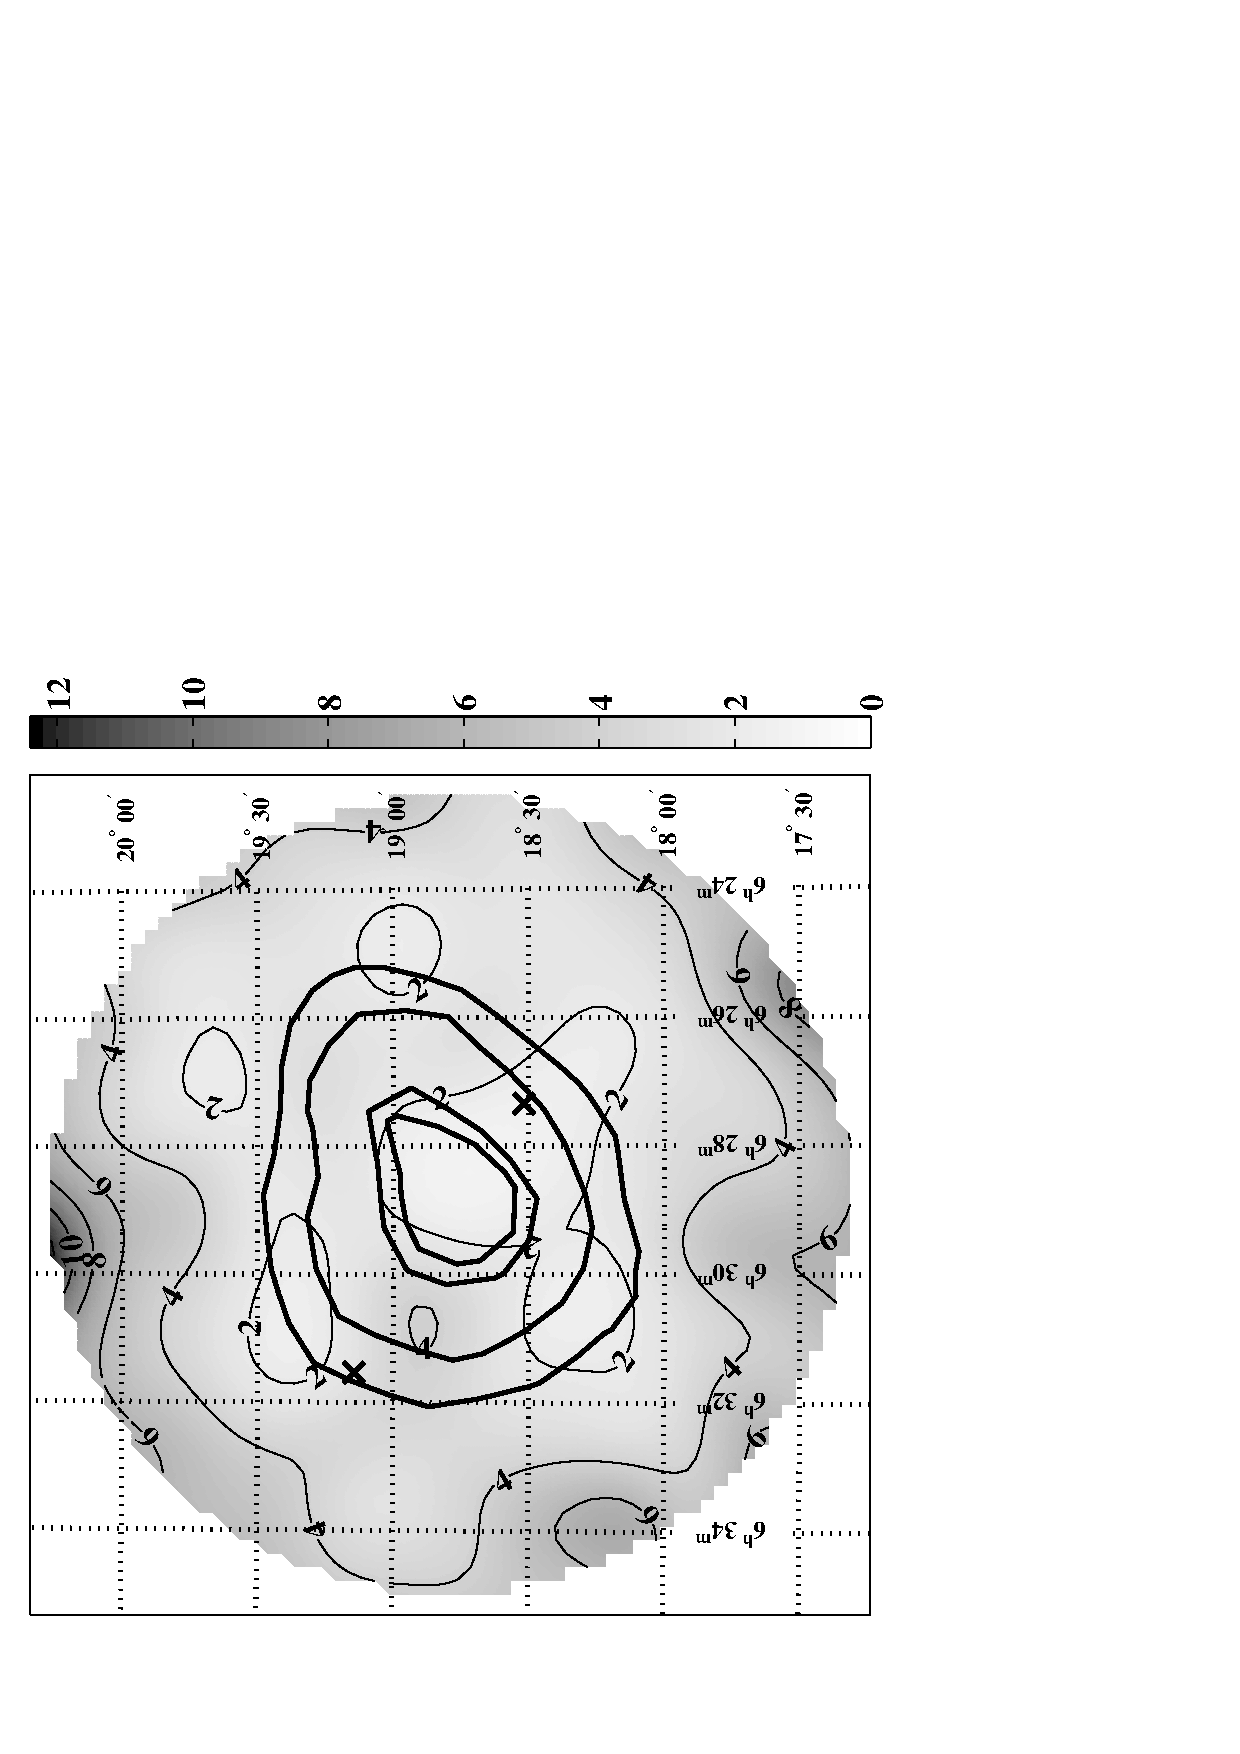
\includegraphics[draft=false,width=\textwidth,angle=270]{plots/chap-observations/loenergy/J0628+1847_sul_conv_bw.pdf}\includegraphics[width=\textwidth,angle=270]{plots/chap-observations/spectra/3EG_J0628+1847.pdf}}
\caption{\label{FIG::OBSERVATIONS::J0628} (Left) Limits on 
emission from 3EG J0628$+$1847 in units of
$10^{-11}$\,cm$^{-2}$\,s$^{-1}$. The 3EG error contours are overlaid
as heavy lines. (Right) Spectrum from the on-line version of the 3EG
catalog with the limit at 350\,GeV.}
\end{figure}

\begin{figure}[p]
\centerline{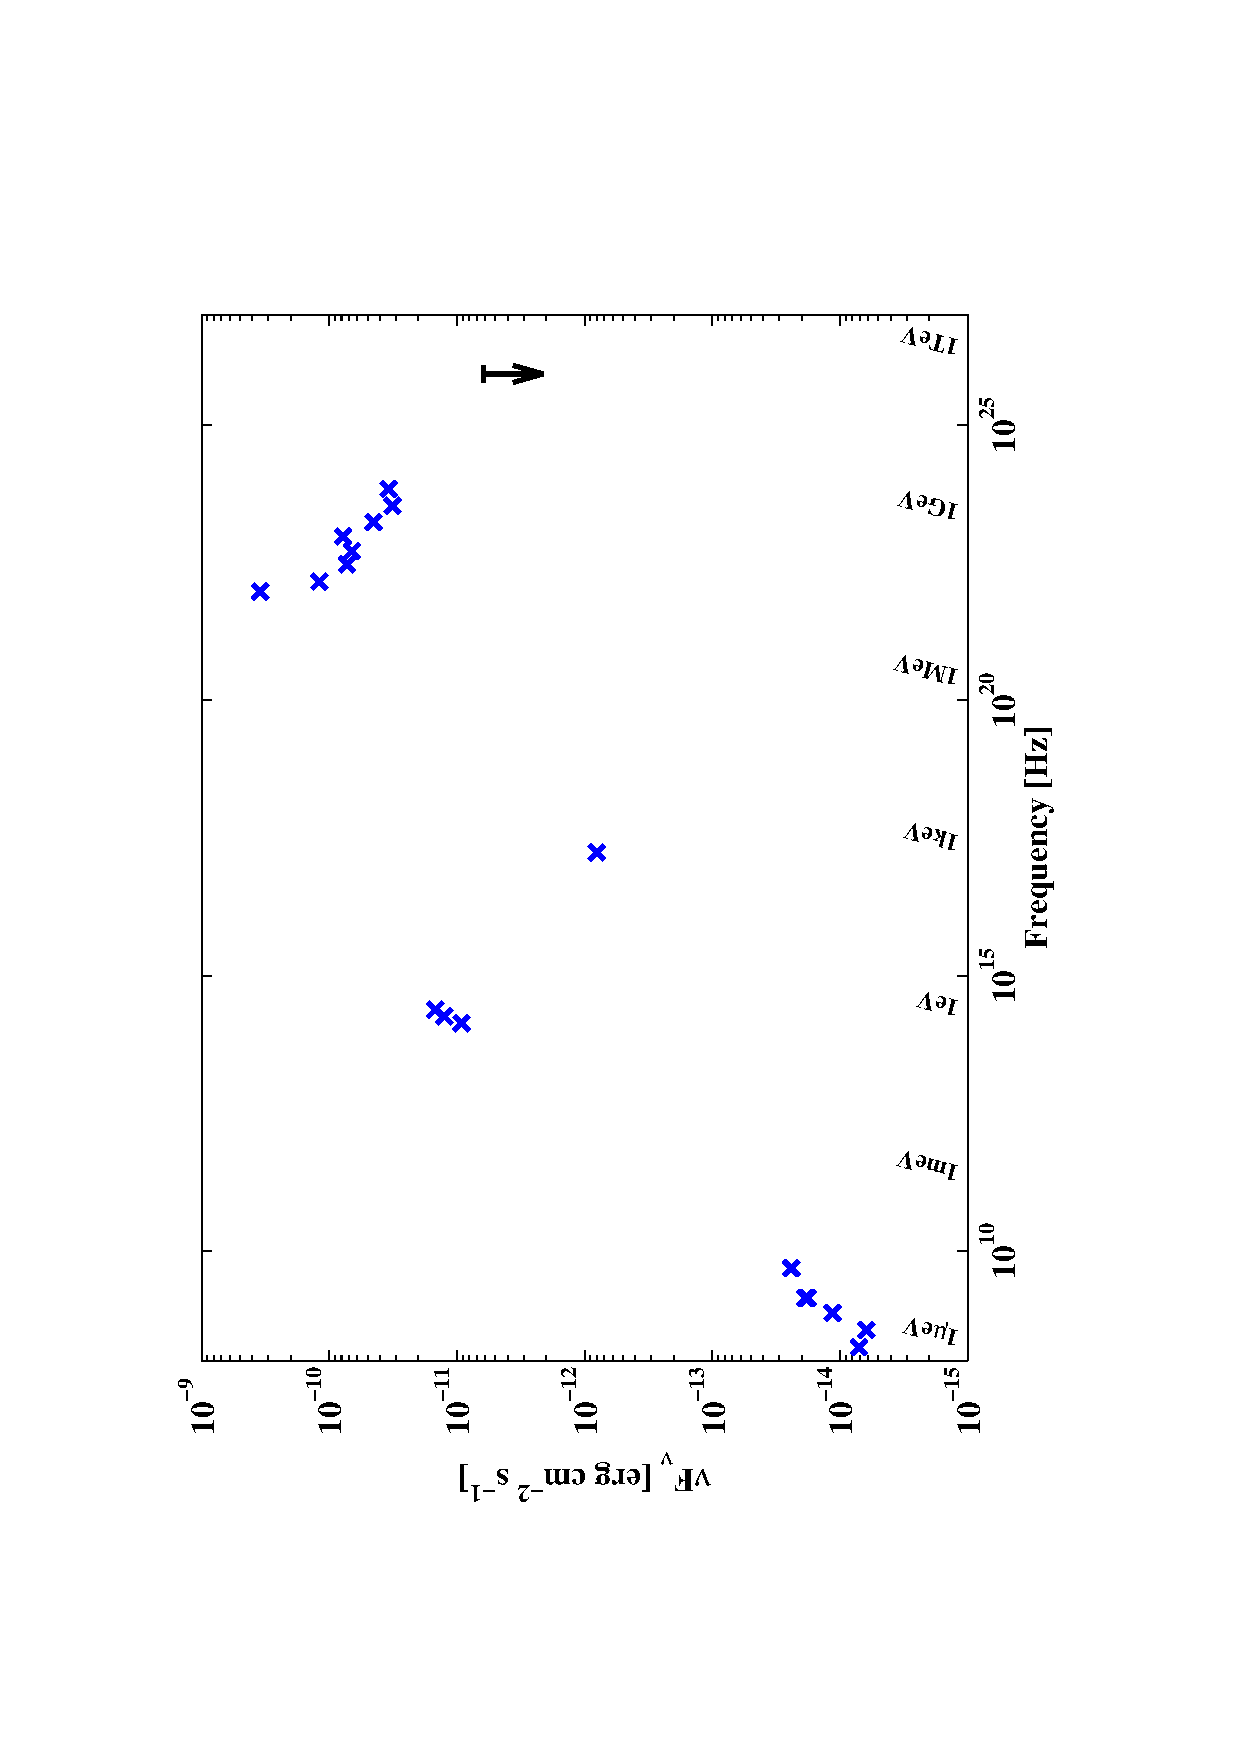
\includegraphics[angle=270,width=0.8\textwidth]{plots/chap-observations/sed0628.pdf}}
\caption{\label{FIG::OBSERVATIONS::SED0628} Spectral energy 
distribution for the radio/x-ray source RX~J0631.4$+$1908
(87GB~0628$+$1911), assuming it is associated with the \Gray
source. The data come from the same sources as in
figure~\ref{FIG::OBSERVATIONS::SED0433}.}
\end{figure}

The \Gray source 3EG~J0628$+$1847 has a relatively weak spectral
index, an average 100\,MeV flux and lies at a low Galactic
latitude. Its variability index could not be determined by
\citet{REF::NOLAN::APJ2003}, since the source failed a consistency
check during their analysis. Despite being close to the Galactic
plane, \citet{REF::ROMERO::AA1999} report no positional associations
with known SNR, OB associations or WR- and O-type
stars. \citet{REF::MATTOX::APJS2001} list two radio sources from the
Green Bank catalog in the field, one just inside the 95\% confidence
contour, the other just inside the 99\% contour; these are listed as
having probabilities of $2\times10^{-4}$ and $9\times10^{-4}$,
respectively, of being counterparts. The second radio source,
87GB~0628$+$1971, is listed as coincident with a ROSAT x-ray source by
\citet{REF::LAURENT_MUEHLEISEN::AAS1997} and has an associated IR 
point source in the 2MASS catalog.

VHE observations of the 3EG source were made between December 2001 and
February 2003. A total of 331\,min.\ of usable data were collected and
analyzed using the two-dimensional technique. No significant emission
was seen in the field; the upper limits on emission that are derived
from the data are presented in figure~\ref{FIG::OBSERVATIONS::J0628}.
The upper limit from within the 95\% error contour is
$F_{(>350\,\mathrm{GeV})}<4.1\times10^{-11}$\,cm$^{-2}$\,s$^{-1}$, and is
displayed with the EGRET spectrum on the right hand side of
figure~\ref{FIG::OBSERVATIONS::J0628}. The VHE upper limit does
not constrain an extrapolation of the EGRET spectrum to 350\,GeV.

The upper limits for the two candidates from
\citet{REF::MATTOX::APJS2001}, are presented in
table~\ref{TAB::OBSERVATIONS::J0628}. Assuming that the
\Gray source is associated with 87GB~0628$+$1911, an approximate SED for the
object is shown in figure~\ref{FIG::OBSERVATIONS::SED0628}. The
distribution shows a bimodal structure, typical of an AGN. Since the
HE component peaks somewhere below 100\,MeV, the source is likely an
LBL. The VHE limit appropriate to the source location does not
significantly constrain the spectrum above 10\,GeV.

\begin{table}[t]
\caption{\label{TAB::OBSERVATIONS::J0628} Upper limits for candidates
in 3EG~J0628$+$1847 field.}
\centerline{\begin{tabular}{lllll}\hline
Source Name & \multicolumn{2}{l}{Coordinates} & Extent & Upper Limit \\
& $\alpha_{2000}$ & $\delta_{2000}$ & deg & $\times10^{-11}$\,cm$^{-2}$\,s$^{-1}$\\\hline
3EG~J0628$+$1847 & $06^h28^m36.1^s$ & $+18^\circ50^{\prime}35^{\prime\prime}$ & 0.66$\times$0.49 & 4.1 \\
87GB~0624$+$1833 & $06^h27^m20.5^s$ & $+18^\circ31^{\prime}04^{\prime\prime}$ & -                & 1.5 \\
87GB~0628$+$1911 & $06^h31^m32.3^s$ & $+19^\circ08^{\prime}41^{\prime\prime}$ & -                & 2.6 \\\hline
\end{tabular}}
\end{table}

\subsection{3EG~J0634$+$0521 and 3EG~J0631$+$0642}

The \Gray sources J0634$+$0521 and J0631$+$0642 both lie in the region of
the Monoceros supernova remnant, although neither is explicitly associated
with it in the 3EG catalog. In addition, the GeV source J0633$+$0645
partially overlaps 3EG~J0631$+$0642 and is listed as a possible
counterpart to the SNR in \citet{REF::LAMB::APJ1997}.

The large shell-type SNR G205.5$+$0.5, or Monoceros Loop Nebula, is 220
arcmin in diameter, the fifth largest SNR in
\citet{REF::GREEN::WEB2001}. The SNR is thought to be
1.39$\pm$0.1\,kpc distant, and approximately $3-20\times 10^4$\,yr in
age, i.e.\ in the Sedov expansion phase. Monoceros was first
recognized as a source of 100\,MeV \Grays by
\citet{REF::ESPOSITO::APJ1996}. \citet{REF::JAFFE::APJ1997} presented a
map of EGRET \Gray emission over a large area around the SNR, where
they found evidence for an extended emission feature in the direction
of the Rossette nebula. They suggest that, since \Gray emission was
not seen uniformly across the remnant, the \Grays are produced in a
region of enhanced shock acceleration at the interaction between the
remnant and the nebula. \citet{REF::KAARET::APJ1999} used the
Beppo-SAX narrow-field instruments to image the region around
J0634$+$0521 and discovered a point source with a hard spectrum,
SAX~J0635$+$0553. They report an optical counterpart, which is likely
a B-type companion star, and conclude that if the \Gray emission is
associated with the system (or a portion of it is), then it is a \Gray
emitting x-ray binary.  When the x-ray observations were subsequently
revisited, a 33.8\,ms\ pulsation was discovered
\citep{REF::KAARET::APJ2000}. In a recent study of all potential EGRET
SNR counterparts,
\citet{REF::TORRES::PR2003}, suggest that the source of the \Gray
emission is far from resolved. The fact that Beppo-SAX did not
discover extended emission from the region, as would be expected in a
shock acceleration scenario, suggests that the binary may be
responsible for the \Gray emission. On the other hand, no orbital
variations are seen in the \Gray signal, arguing against an origin in
the binary system.  Analysis of the pulsar energetics and accretion
rate further confuses the issue, see \citet{REF::TORRES::PR2003} for
review. \citet{REF::LUCARELLI::HEGR2001} report preliminary evidence
for VHE \Gray emission from the region with the HEGRA telescope
system\footnote{At a $5.7\sigma$ level for emission based on
120\,hrs.\ at $E>500$\,GeV from four $0.2^\circ\times0.2^\circ$ bins
in the region of the Rossette nebula.}. The VHE emission was extended
and was not coincidental with the Beppo-SAX source. No flux was
reported for the observations.

\citet{REF::TORRES::PR2003} suggest that 3EG~J0643$+$0521 might be a
composite source, with the Beppo-SAX source being responsible for a
portion of the EGRET \Gray flux and the bulk of the x-ray emission,
while interactions between the SNR and the Rossette nebula may
contribute to the 3EG flux and account for any VHE emission. They
predict that, if a composite source is responsible, a spectral break
should be detected between the EGRET and ground-based \Gray regimes. For
3EG~J0631$+$0642 a pure shock acceleration model is sufficient to
explain the 3EG flux.

\citet{REF::ROMERO::AA1999} studied potential positional associations
between 3EG sources and SNR, OB associations, WR-type and O-type
stars.  In addition to the Monoceros SNR, they report two O-type stars
and two OB associations in the region: from a catalog of O-type stars
\citep{REF::CRUZ-GONZALEZ::RMAA1974} HD46150 and HD46223 and
from a catalog of OB-associations \citep{REF::MELNIK::AL1995}
Mon~OB~2A and Mon~OB~1B\footnote{\citet{REF::ROMERO::AA1999} refer to
Mon~OB~2B which is not in the catalog. Mon~OB~1B is the correct source
association.}. Mon~OB~1B lies just outside of the region studied in
this work.

The VHE observations of this source consist of 248\,min.\ of data. In
order to accomodate the 95\% confidence contours of both 3EG sources
and the GeV source, the telescope was pointed close to the coordinates
listed for the Monoceros nebula in \citet{REF::GREEN::WEB2001},
approximately half way between the two 3EG sources. Although both
EGRET sources were in the field of view they lie toward the edge of
the camera, which is less sensitive to \Grays than the center.

No significant emission was detected in the field;
figure~\ref{FIG::OBSERVATIONS::J0634UL} presents the upper limits
derived from the observations. The figure shows the EGRET contours for
both sources, with 3EG~J0634$+$0521 toward the lower left. The GeV
source is indicated as a dashed circle overlapping 3EG~J0631$+$0642.
The dash-dotted circle towards the bottom of the figure indicates the
location of Mon~OB~2A, with the two O-type stars, each marked by an
``X'' within. Finally, the location of SAX~J0635$+$0533 is marked as
an ``X'' near the center of
3EG~J0634$+$0521. Table~\ref{TAB::OBSERVATIONS::J0634} summarizes the
upper limits derived for the EGRET error-boxes and for the various
candidate sources.

\begin{table}[t]
\caption{\label{TAB::OBSERVATIONS::J0634} Upper limits for candidates
in the fields of 3EG J0634$+$0521 and 3EG J0631$+$0642.}
\centerline{\begin{tabular}{lllll}\hline
Source Name & \multicolumn{2}{l}{Coordinates} & Extent & Upper Limit \\
& $\alpha_{2000}$ & $\delta_{2000}$ & deg & $\times10^{-11}$\,cm$^{-2}$\,s$^{-1}$\\\hline
3EG~J0634$+$0521 & $06^h34^m39.9^s$ & $+05^\circ28^{\prime}21^{\prime\prime}$ & $0.85\times0.50$ & 5.3 \\
3EG~J0631$+$0642 & $06^h31^m39.4^s$ & $+06^\circ41^{\prime}42^{\prime\prime}$ & $0.55\times0.39$ & 6.0 \\
GeV~J0633$+$0645 & $06^h33^m08.8^s$ & $+06^\circ45^{\prime}49^{\prime\prime}$ & $0.42\times0.42$ & 4.9 \\
SAX~J0635$+$0533 & $06^h35^m17.4^s$ & $+05^\circ33^{\prime}21^{\prime\prime}$ & -                & 2.0 \\
Mon~OB~2A        & $06^h32^m10.2^s$ & $+04^\circ50^{\prime}46^{\prime\prime}$ & $0.33\times0.47$ & 4.7 \\
HD46150          & $06^h30^m36.0^s$ & $+04^\circ57^{\prime}00^{\prime\prime}$ & -                & 3.1 \\
HD46223          & $06^h31^m00.0^s$ & $+04^\circ50^{\prime}00^{\prime\prime}$ & -                & 2.4 \\\hline
\end{tabular}}
\end{table}

\begin{figure}[p]
\centerline{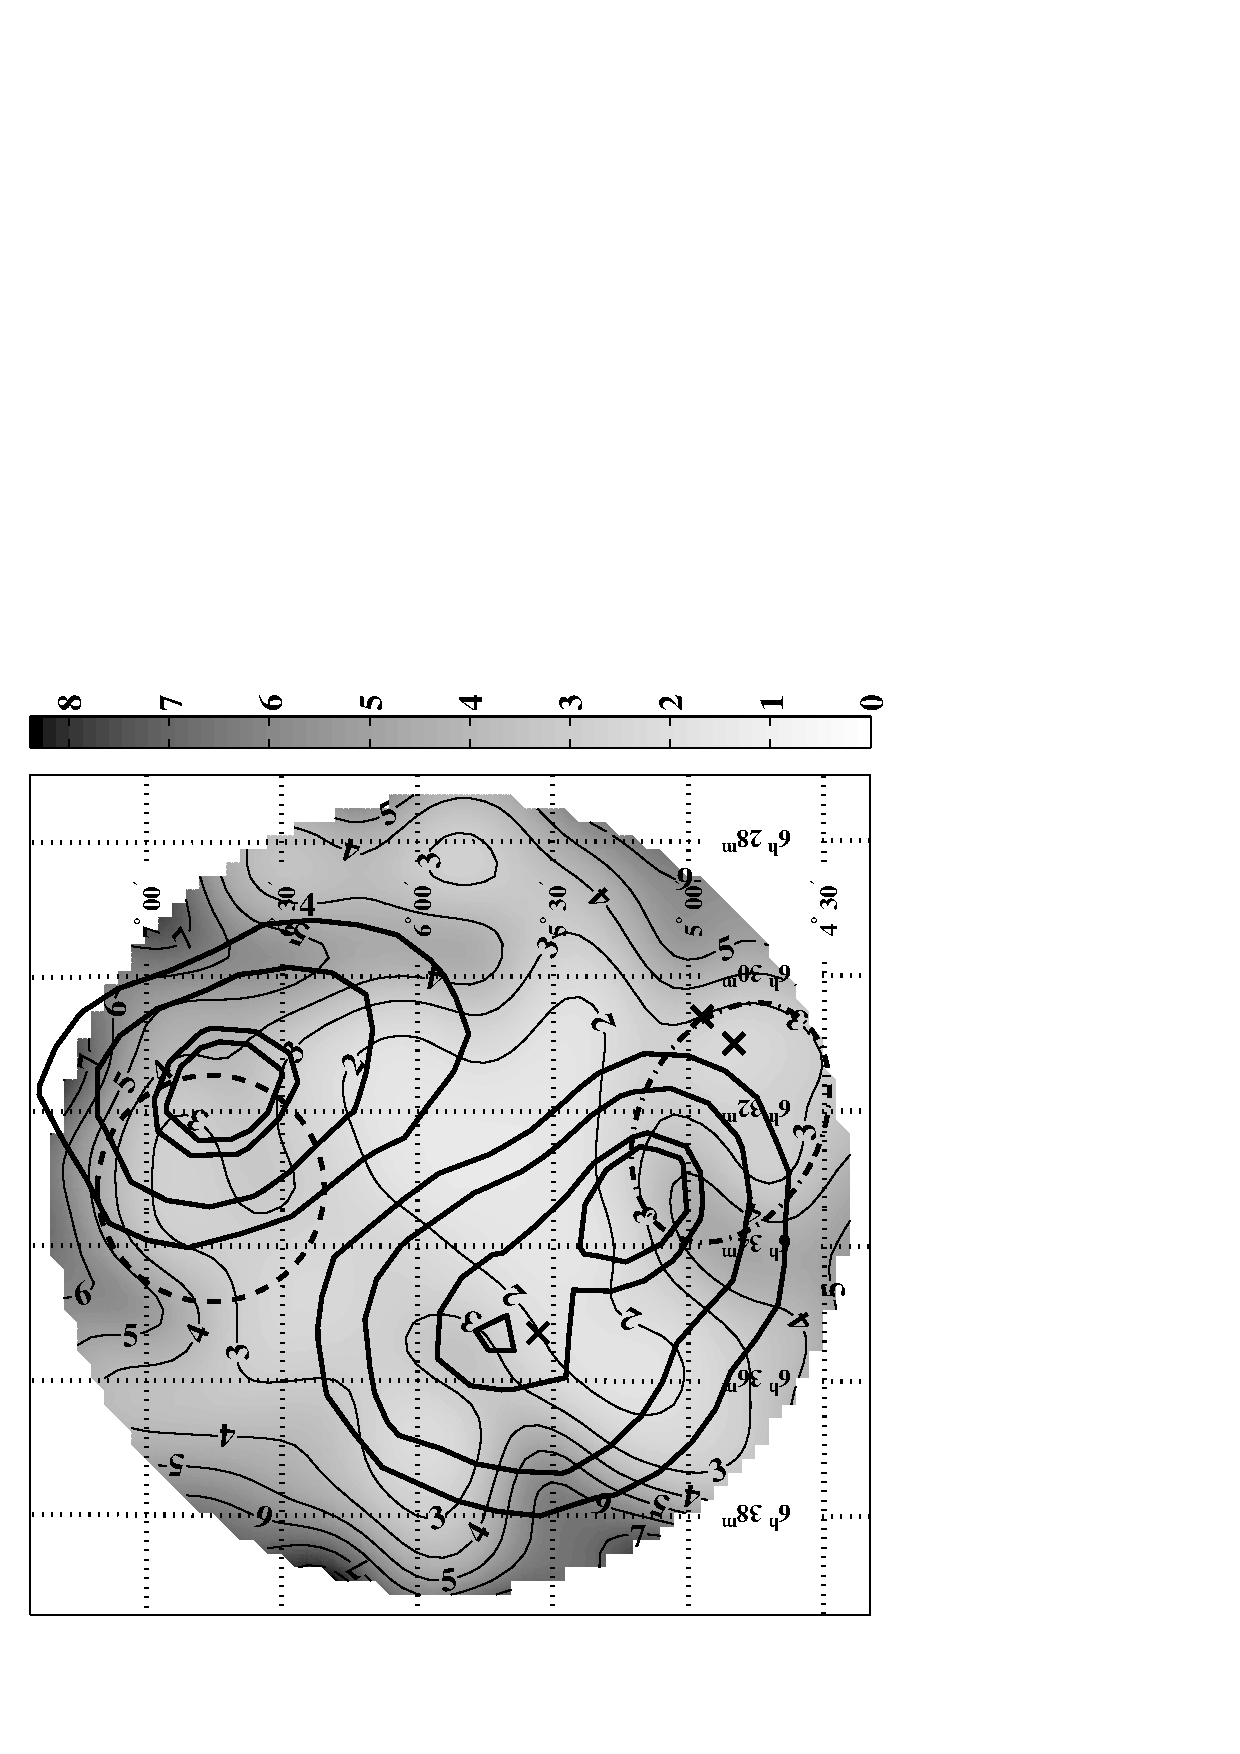
\includegraphics[draft=false,angle=270,width=0.75\textwidth]{plots/chap-observations/loenergy/J0634+0521_sul_conv_bw.pdf}}
\caption{\label{FIG::OBSERVATIONS::J0634UL} Upper limits on emission 
from 3EG~J0634$+$0521, 3EG~J0631$+$0642 and GeV~J0633$+$0645 in units of
$10^{-11}$\,cm$^{-2}$\,s$^{-1}$. The 3EG error contours are overlaid
as heavy lines, the GeV error circle as a dashed line toward the top
of the diagram. The dash-dotted ellipse toward the bottom of the figure
indicates the OB association Mon~OB~2A.}
\end{figure}

\begin{figure}[p]
\includegraphics[angle=270,width=0.49\textwidth]{plots/chap-observations/spectra/3EG_J0634+0521.pdf}\hspace*{\fill}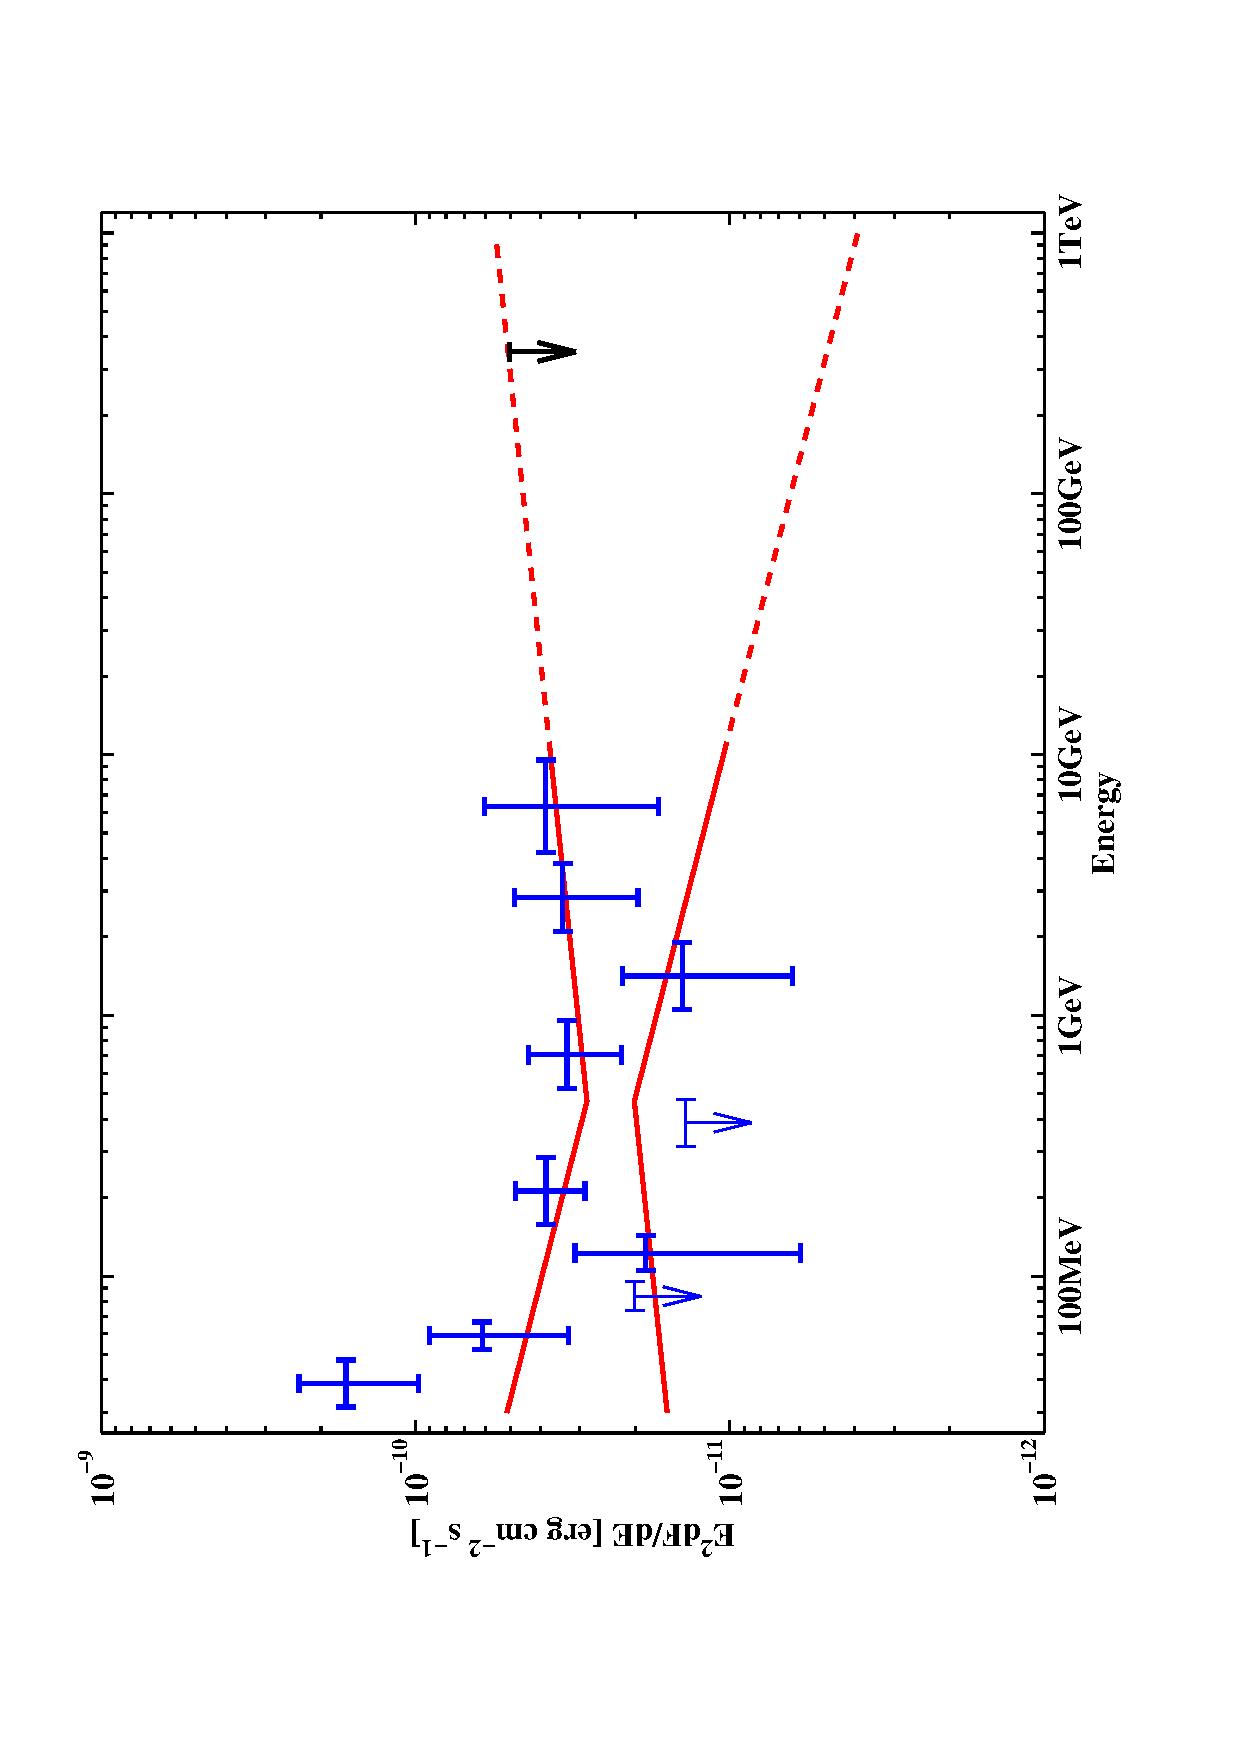
\includegraphics[angle=270,width=0.49\textwidth]{plots/chap-observations/spectra/3EG_J0631+0642.pdf}
\caption{\label{FIG::OBSERVATIONS::J0634SPEC} Spectrum for 
3EG~J0634$+$0521 (left) and 3EG~J0631$+$0642 (right) from on-line
version of the 3EG catalog with the upper limit at 350\,GeV. The limit
at 500\,GeV from \citet{REF::LESSARD::ICRC1999} is also indicated.}
\end{figure}

The extrapolated EGRET spectra for both sources are shown in
figure~\ref{FIG::OBSERVATIONS::J0634SPEC} with the upper limits at
350\,GeV. These observations do not require a break in the spectrum of
either source and cannot substantiate (or refute) the two component
model of \citet{REF::TORRES::PR2003}. Although the previous upper
limits derived from observations with the Whipple telescope
\citep{REF::LESSARD::ICRC1999} had a lower flux value, the
observations were made at higher energy, and do not constrain the
extrapolated EGRET spectrum any more than these observations. The
previous limits are shown on the figure at 500\,GeV, at approximately
the same level. This source is a prime candidate for observation with
the next generation of ground-based instruments, such as VERITAS,
which will have an order of magnitude increase in sensitivity over the
current generation, and will operate at at energies
$\sim100$\,GeV. These instruments will have the ability to accurately
reconstruct the origin of the {\Grayc}s, and will have the ability to
resolve the \Gray emission from unidentified EGRET sources such as
this one.

\subsection{3EG~J1009$+$4855}

In the 3EG catalog, J1009$+$4855 is listed as having a low flux and a
hard, but relatively ill defined, spectral
index. \citet{REF::NOLAN::APJ2003} present only an upper limit for the
variability index, not surprising given the low mean flux from the
source and that it was not seen at a particularly high flux state during
any of the EGRET viewing periods. The source is also listed in the GeV
catalog as a low significance source. Very little is known about this source
at other wavelengths, the EGRET catalog suggests a weak association
with the radio/x-ray source B1011+496, a known AGN at redshift of
$z=0.2$. \citet{REF::MATTOX::APJS2001} lists the probability of that
association as $2\times10^{-4}$; the radio-source lies outside of
the large 99\% error contour\footnote{The EGRET contours are derived
from rectangular likelihood maps in Galactic or equatorial coordinates
\citep[see][]{REF::MATTOX::APJ1996}. The 95\% and 99\% confidence
contours are not bounded within the map for this source and hence are
not closed in figure~\ref{FIG::OBSERVATIONS::J1009}.} and the
association seems unlikely.

\begin{figure}[t]
\resizebox*{\textwidth}{!}{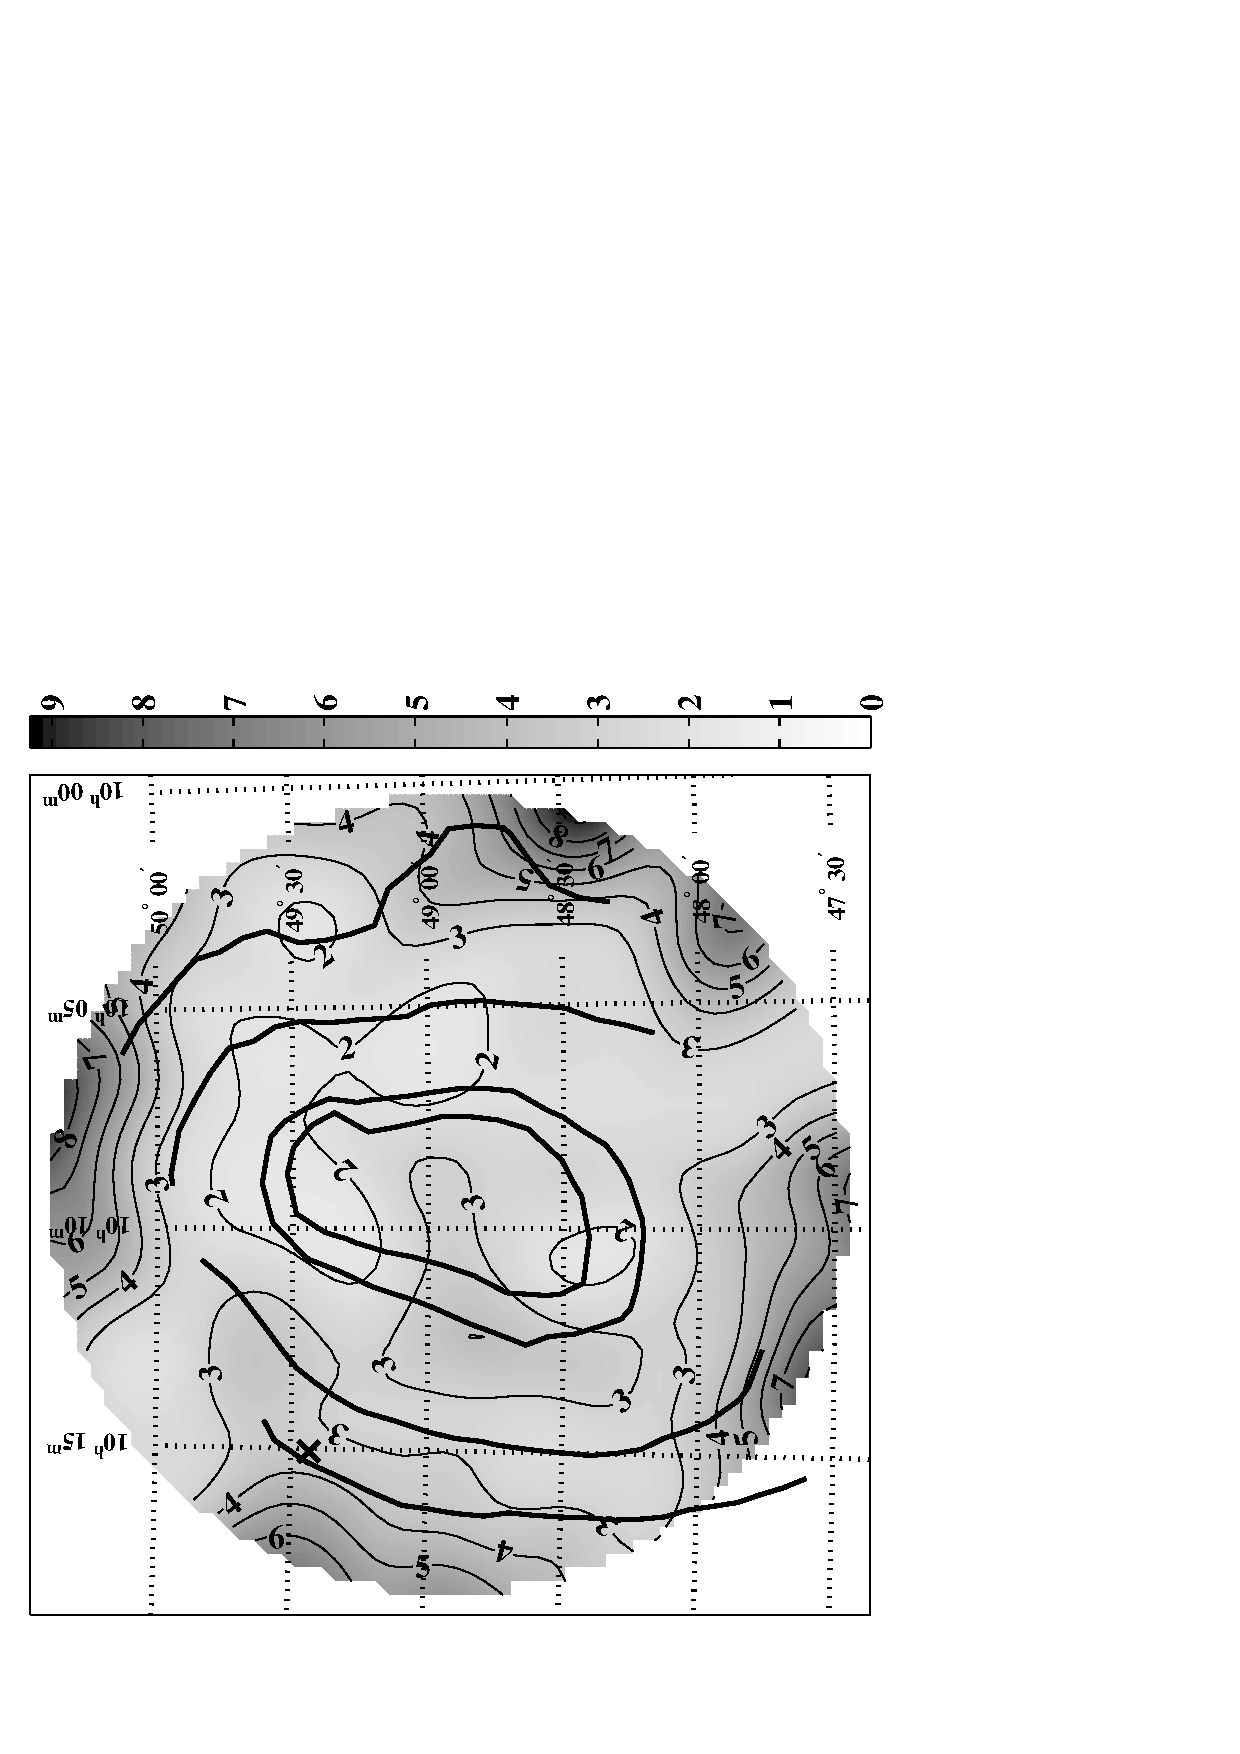
\includegraphics[draft=false,width=\textwidth,angle=270]{plots/chap-observations/loenergy/J1009+4855_sul_conv_bw.pdf}\includegraphics[width=\textwidth,angle=270]{plots/chap-observations/spectra/3EG_J1009+4855.pdf}}
\caption{\label{FIG::OBSERVATIONS::J1009} (Left) Limits on 
emission from 3EG J1009$+$4855 in units of
$10^{-11}$\,cm$^{-2}$\,s$^{-1}$. The 3EG error contours are overlaid
as heavy lines. (Right) Spectrum from the on-line version of the 3EG
catalog with the limit at 350\,GeV.}
\end{figure}

\begin{table}[t!]
\caption{\label{TAB::OBSERVATIONS::J1009} Upper limits for candidates
in 3EG~J1009$+$4855 field.}
\centerline{\begin{tabular}{lllll}\hline
Source Name & \multicolumn{2}{l}{Coordinates} & Extent & Upper Limit \\
& $\alpha_{2000}$ & $\delta_{2000}$ & deg & $\times10^{-11}$\,cm$^{-2}$\,s$^{-1}$\\\hline
3EG~J1009$+$4855 & $10^h09^m59.3^s$ & $+48^\circ50^{\prime}30^{\prime\prime}$ & $1.12\times0.80$ & 4.6 \\
87GB~1011$+$4941 & $10^h15^m04.1^s$ & $+49^\circ26^{\prime}01^{\prime\prime}$ & -                & 3.3 \\\hline
\end{tabular}}
\end{table}

VHE observations of the source were made between December 2001 and
March 2002. A total of 248\,min.\ of usable data were obtained, pointed
at the center of the 3EG source. No significant emission was detected,
a map of the upper limits on emission from the region is presented in
figure~\ref{FIG::OBSERVATIONS::J1009}. A limit of
$F_{(>350\,\mathrm{GeV})}<4.6\times10^{-11}$\,cm$^{-2}$\,s$^{-1}$ is placed on
emission within the 95\% error contour,
% and of $F_{(>350\,\mathrm{GeV})}<3.3\times10^{-11}$\,cm$^{-2}$\,s$^{-1}$ on emission
%from the radio source. 
shown with an extrapolation of the EGRET spectrum in
figure~\ref{FIG::OBSERVATIONS::J1009}.  The upper limit does not
significantly constrain the wide range of fluxes
% at 350\,GeV (covering two orders of magnitude) 
allowed by the large uncertainties in the 3EG spectrum.

\subsection{3EG~J1323$+$2200}

EGRET detected variable emission from the high latitude source
J1323$+$2200, with an average flux of
$5.2\pm1.6\times10^{-8}$\,cm$^{-2}$\,s$^{-1}$. During most of the
viewing periods (VP) for which it was in the field of view no emission
was detected; during VP~308.0 a flux of
$68.4\pm22.6\times10^{-8}$\,cm$^{-2}$\,s$^{-1}$ was measured. The
source is listed in the GeV catalog as a ``source of GeV gamma rays
based upon the search for repeating, weak
outbursts''. \citet{REF::NOLAN::APJ2003} calculate the variability
index to be 1.09, consistent with a highly variable source. Its
100\,MeV spectral index is hard, with a relatively large error,
$\Gamma=1.86\pm0.35$. \citet{REF::MATTOX::APJS2001} lists four
potential associations with radio sources, two of which (with the
lowest 5\,GHz fluxes) are within the 95\% confidence contour. The most
likely association, just outside of the 95\% contour, is listed as
having a probability of $\sim1\%$.

\begin{figure}[b]
\resizebox*{\textwidth}{!}{\includegraphics[draft=false,width=\textwidth,angle=270]{plots/chap-observations/loenergy/J1323+2200_sul_conv_bw.pdf}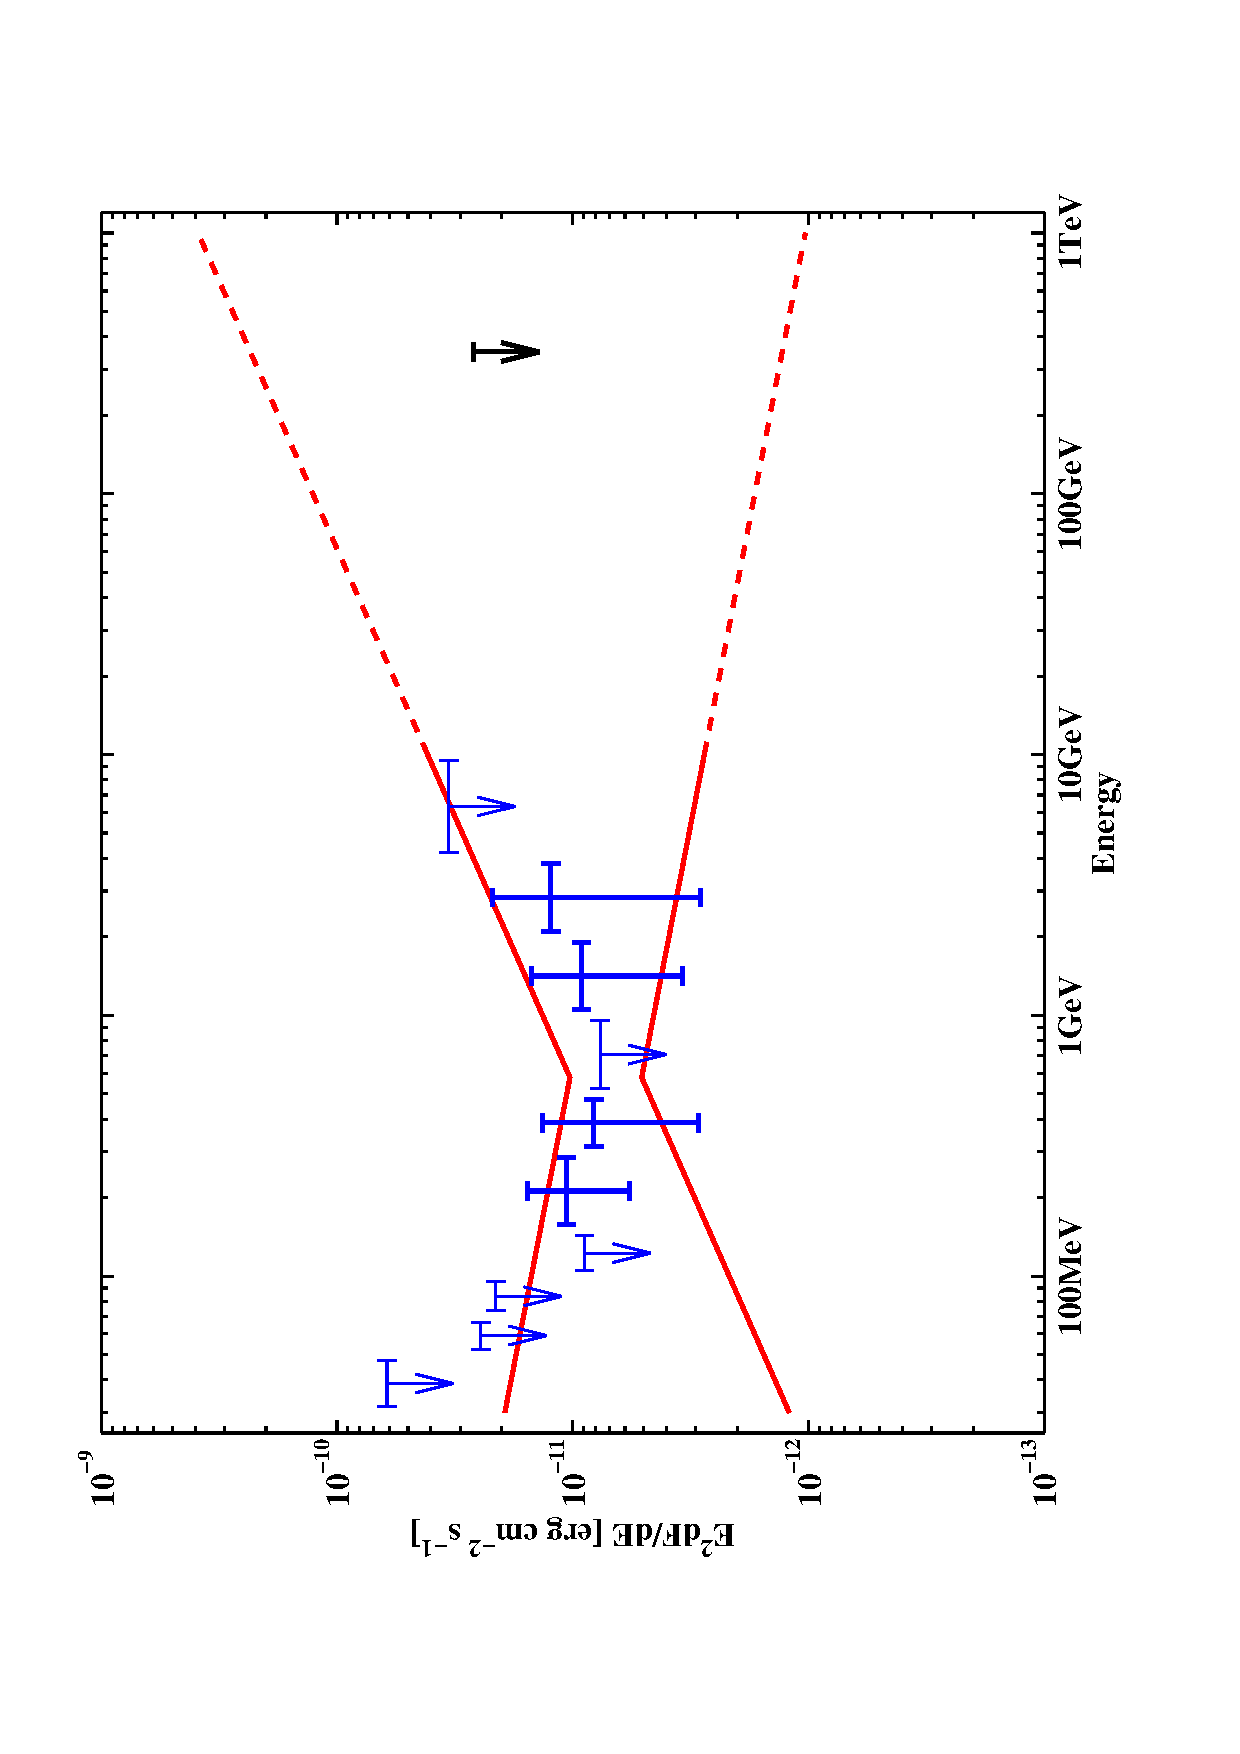
\includegraphics[width=\textwidth,angle=270]{plots/chap-observations/spectra/3EG_J1323+2200.pdf}}
\caption{\label{FIG::OBSERVATIONS::J1323} (Left) Limits on 
emission from 3EG~J1323$+$2200 in units of
$10^{-11}$\,cm$^{-2}$\,s$^{-1}$. The 3EG error contours are overlaid
as heavy lines. (Right) Spectrum from the on-line version of the 3EG
catalog with the limit at 350\,GeV.}
\end{figure}

\begin{table}[t]
\caption{\label{TAB::OBSERVATIONS::J1323} Upper limits for candidates
in 3EG~J1323$+$2200 field.}
\centerline{\begin{tabular}{lllll}\hline
Source Name & \multicolumn{2}{l}{Coordinates} & Extent & Upper Limit \\
& $\alpha_{2000}$ & $\delta_{2000}$ & deg & $\times10^{-11}$\,cm$^{-2}$\,s$^{-1}$\\\hline
3EG~J1323$+$2200 & $13^h23^m20.1^s$ & $+22^\circ02^{\prime}52^{\prime\prime}$ & $0.52\times0.43$ & 3.1 \\
87GB~1324$+$2226 & $13^h27^m00.8^s$ & $+22^\circ10^{\prime}50^{\prime\prime}$ & -                & 2.1 \\
87GB~1318$+$2231 & $13^h21^m11.2^s$ & $+22^\circ16^{\prime}12^{\prime\prime}$ & -                & 2.1 \\
87GB~1319$+$2203 & $13^h22^m11.4^s$ & $+21^\circ48^{\prime}12^{\prime\prime}$ & -                & 1.6 \\
87GB~1321$+$2229 & $13^h24^m14.9^s$ & $+22^\circ13^{\prime}08^{\prime\prime}$ & -                & 1.2 \\\hline
\end{tabular}}
\end{table}

VHE observations during the first five months of 2001 resulted in
276\,min.\ of usable data centered on the 3EG catalog position. The
data were analyzed using the two dimensional reconstruction technique
and no significant emission was detected from the source. Upper limits
on emission are presented in figure~\ref{FIG::OBSERVATIONS::J1323}. A
limit of
$F_{(>350\,\mathrm{GeV})}<3.1\times10^{-11}$\,cm$^{-2}$\,s$^{-1}$ is
placed on emission within the 95\% error contour, limits on the four
radio sources, which are displayed as crosses in the figure, are
listed in table~\ref{TAB::OBSERVATIONS::J1323}. The limits do not
significantly constrain an extrapolation of the EGRET spectrum to
350\,GeV.

\subsection{3EG~J1337$+$5029}

The \Gray source 3EG~J1337$+$5029, at Galactic latitude of
$+65^\circ$, was detected by EGRET with a relatively low flux of
$9.2\pm2.6\times10^{-8}$\,cm$^{-2}$\,s$^{-1}$ and a hard spectrum of
$1.83\pm0.29$, the fourth hardest among the unidentified
sources. \citet{REF::NOLAN::APJ2003} list a variability index of 0.53,
indicating a variable source; it was detected significantly in four of
the six viewing periods that it was in the EGRET field of view.

\citet{REF::COLAFRANCESCO::AA2002} suggests that the \Gray source is
associated with the galaxy cluster Abell~1758
\citep{REF::ABELL::APJS1989}, with diameter of 22\,arcmin and
redshift of $z=0.279$. The cluster is coincident with two ROSAT x-ray
sources RX~J1332.5+5024 and RX~J1332.7+5032, both of which show
evidence of being extended, each with a radius of approximately
75\,arcsec. \citet{REF::BOHRINGER::APJS2000} present a reanalysis of
the x-ray data for all extended RASS-BSC sources, accounting properly
for the extended nature of the source in the flux calculation. They
calculate a flux of
$F_{\mathrm{X}}(0.1-2.4\,\mathrm{keV})=5.6\pm0.53\times10^{-12}$\,erg\,cm$^{-2}$\,s$^{-1}$
for the cluster\footnote{They label the source as RXC~1332+5032;
seemingly it corresponds to both of the RASS-BSC sources. The x-ray
flux they quote was been integrated over a radius of 11.5\,arcmin,
covering the whole extent of the cluster.}, corresponding to a
luminosity of
$L_{\mathrm{X}}(0.1-2.4\,\mathrm{keV})\sim1.8\times10^{45}$\,erg\,s$^{-1}$.
Additionally, four radio sources from the NRAO VLA Sky Survey (NVSS) are
coincident with the cluster. \citet{REF::COLAFRANCESCO::AA2002}
concludes that since the cluster ``falls within the 95\% confidence
level position error contour of the source'' and, given the x-ray/radio
sources listed above, this source represents a ``probable candidate for
the correlation of galaxy clusters and EGRET unidentified \Gray
sources''.  Analysis of the 3EG significance maps performed for this
study shows that the cluster location, as listed in
\citet{REF::ABELL::APJS1989} and the NED database, does not lie within
the 95\% contour, even taking into account the diameter of the
cluster.  Figure~\ref{FIG::OBSERVATIONS::J1337SIGMA} shows that the
cluster lies just outside the 95\% contour to the west\footnote{By
convention, astronomical maps have west and east reversed with respect
to the usual mapping convention. They are oriented to coincide with
what someone on the ground looking up at the sky would see, with north
pointed up.}, approximately $0.8^\circ$ from the 3EG catalog position.

There are five additional RASS-BSC x-ray sources in the field, four
within the 95\% contour; some have radio counterparts in the NVSS.
The RASS catalog lists some potential associations for the x-ray
sources, two with stars, and one with an AGN and a star. Limits are
presented for each of the x-ray sources irrespective of these
associations. \citet{REF::MATTOX::APJS2001} list two unlikely radio
associations from the Green Bank catalog, one outside of the 99\%
contour, the other just inside. These seven sources are shown on
figure~\ref{FIG::OBSERVATIONS::J1337SIGMA}. The two x-ray sources
inside the cluster have been omitted in light of the combined,
extended source discussed above \citep{REF::BOHRINGER::APJS2000}.

VHE observations during the first six months of 2002 yielded
166\,min.\ of data. Figure~\ref{FIG::OBSERVATIONS::J1337SIGMA} shows
the significance of excess (or deficit) {\Grayc}-like events within
the field of view. A broad excess, approximately
$1.0^\circ\times0.5^\circ$ in extent, lies along the 99\% contour to
the north-west of the 3EG catalog position. The peak in the excess has
an a priori statistical significance of $\sim4\sigma$, making it the
most significant of all the observations in this survey. Since
emission was not predicted from this particular location a priori, the
true probability of obtaining such a result by chance, given the
number of sources observed in this survey and the combined size of the
EGRET error-boxes must be evaluated. This is done by first calculating
the number of ``independent'' $0.1^\circ\times0.1^\circ$ bins
represented by the sources using
figure~\ref{FIG::ANALYSIS::NINDEPENDENTLIKELIHOOD}. It is estimated
that $\sim200$ bins lie within the 95\% contours for the 18 sources
analyzed using the two dimensional
technique. Figure~\ref{FIG::ANALYSIS::SIGMASIGMA} can then be used to
calculate an equivalent Gaussian significance of the probability of
obtaining such a result by chance. In the case of a $4\sigma$ excess
with 200 trials, the equivalent significance is
$\sim2.5\sigma$\footnote{Strictly, the excess seen here is not within
the 95\% contour; a similar calculation for all of the bins within
$1.1^\circ$ of the center of the 18 sources gives 600 trials and a
significance of $\sim2.1\sigma$.}. Given this conservative approach
and that the the dataset for this source is so small ($\sim$2.5\,hrs),
we do not claim to have seen emission from this source. However, the
excess gives an a priori expectation of emission from this location,
and is a strong reason to make followup observations. Results from
these independent observations will then not have to pay a
``statistical penalty''. Based on these results, the source has been
awarded 20\,hrs of observations with the Whipple telescope during
spring 2004.

\begin{table}[t]
\caption{\label{TAB::OBSERVATIONS::J1337} Upper limits for candidates
in 3EG~J1337$+$5029 field.}
\centerline{\begin{tabular}{lllll}\hline
Source Name & \multicolumn{2}{l}{Coordinates} & Extent & Upper Limit \\
& $\alpha_{2000}$  & $\delta_{2000}$ & deg & $\times10^{-11}$\,cm$^{-2}$\,s$^{-1}$\\\hline
3EG~J1337$+$5029        & $13^h38^m00.8^s$ & $+50^\circ25^{\prime}57^{\prime\prime}$ & $0.77\times0.66$ & 5.9 \\
Abell~1758              & $13^h32^m31.7^s$ & $+50^\circ30^{\prime}41^{\prime\prime}$ & $0.18\times0.18$ & 6.9 \\
87GB~1329$+$5023        & $13^h31^m37.2^s$ & $+50^\circ07^{\prime}55^{\prime\prime}$ & -                & 3.6 \\
87GB~1340$+$5125        & $13^h42^m23.5^s$ & $+51^\circ10^{\prime}18^{\prime\prime}$ & -                & 3.9 \\
% CLUSTER $^*$J133230.8$+$502436 & $13^h32^m30.8^s$ & $+50^\circ24^{\prime}36^{\prime\prime}$ & -                & 5.8 \\
% CLUSTER $^*$J133243.3$+$503256 & $13^h32^m43.3^s$ & $+50^\circ32^{\prime}56^{\prime\prime}$ -                & & 6.1 \\
$^*$J133510.2$+$503920 & $13^h35^m10.2^s$ & $+50^\circ39^{\prime}20^{\prime\prime}$ & -                & 3.5 \\
RX~J1335.3$+$5015       & $13^h35^m19.6^s$ & $+50^\circ15^{\prime}04^{\prime\prime}$ & -                & 3.0 \\
RX~J1337.3$+$5032       & $13^h37^m20.0^s$ & $+50^\circ32^{\prime}52^{\prime\prime}$ & -                & 2.5 \\
% RXJ SOURCE ABOVE $^*$J133519.6$+$501504 & $13^h35^m19.6^s$ & $+50^\circ15^{\prime}04^{\prime\prime}$ & -                & 3.0 \\
% RXJ SOURCE ABOVE $^*$J133720.0$+$503252 & $13^h37^m20.0^s$ & $+50^\circ32^{\prime}52^{\prime\prime}$ & -                & 2.5 \\
$^*$J134023.3$+$503113 & $13^h40^m23.3^s$ & $+50^\circ31^{\prime}13^{\prime\prime}$ & -                & 2.1 \\
$^*$J134350.8$+$503016 & $13^h43^m50.8^s$ & $+50^\circ30^{\prime}16^{\prime\prime}$ & -                & 3.0 \\\hline
\end{tabular}}
\centerline{\footnotesize{\begin{tabular}{p{0.9\textwidth}}
$^*$ The standard RASS-BSC catalog prefix of 1RXS is omitted for formatting purposes.\\
\end{tabular}}}
\end{table}

\begin{figure}[p]
\centerline{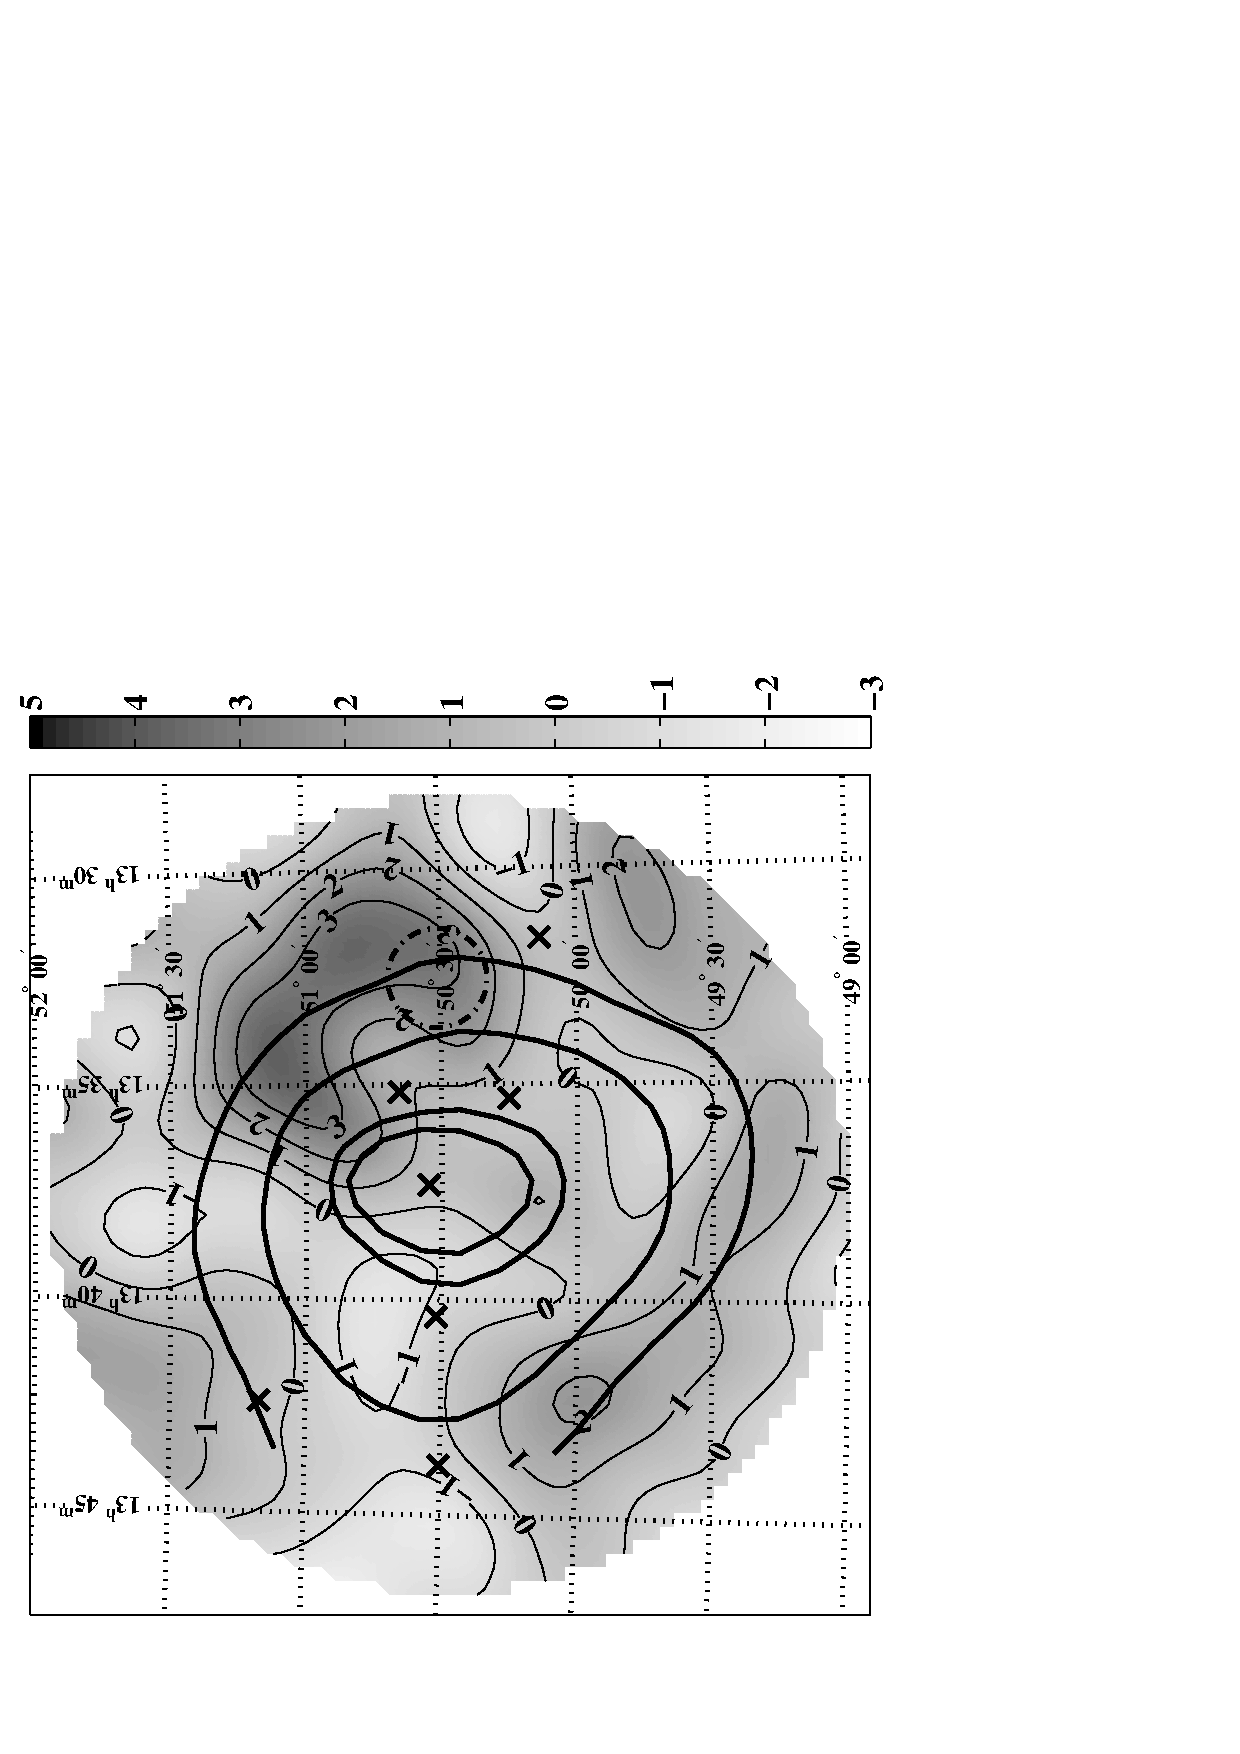
\includegraphics[draft=false,angle=270,width=0.75\textwidth]{plots/chap-observations/loenergy/J1337+5029_sigma_conv_bw.pdf}}
\caption{\label{FIG::OBSERVATIONS::J1337SIGMA} Significance of excess
{\Grayc}-like events detected from the region of 3EG J1337$+$5029. The
cluseter is shown as a dot-dashed circle, and the various other sources
in the field as ``X'' marks.}
\end{figure}

\begin{figure}[p]
\resizebox*{\textwidth}{!}{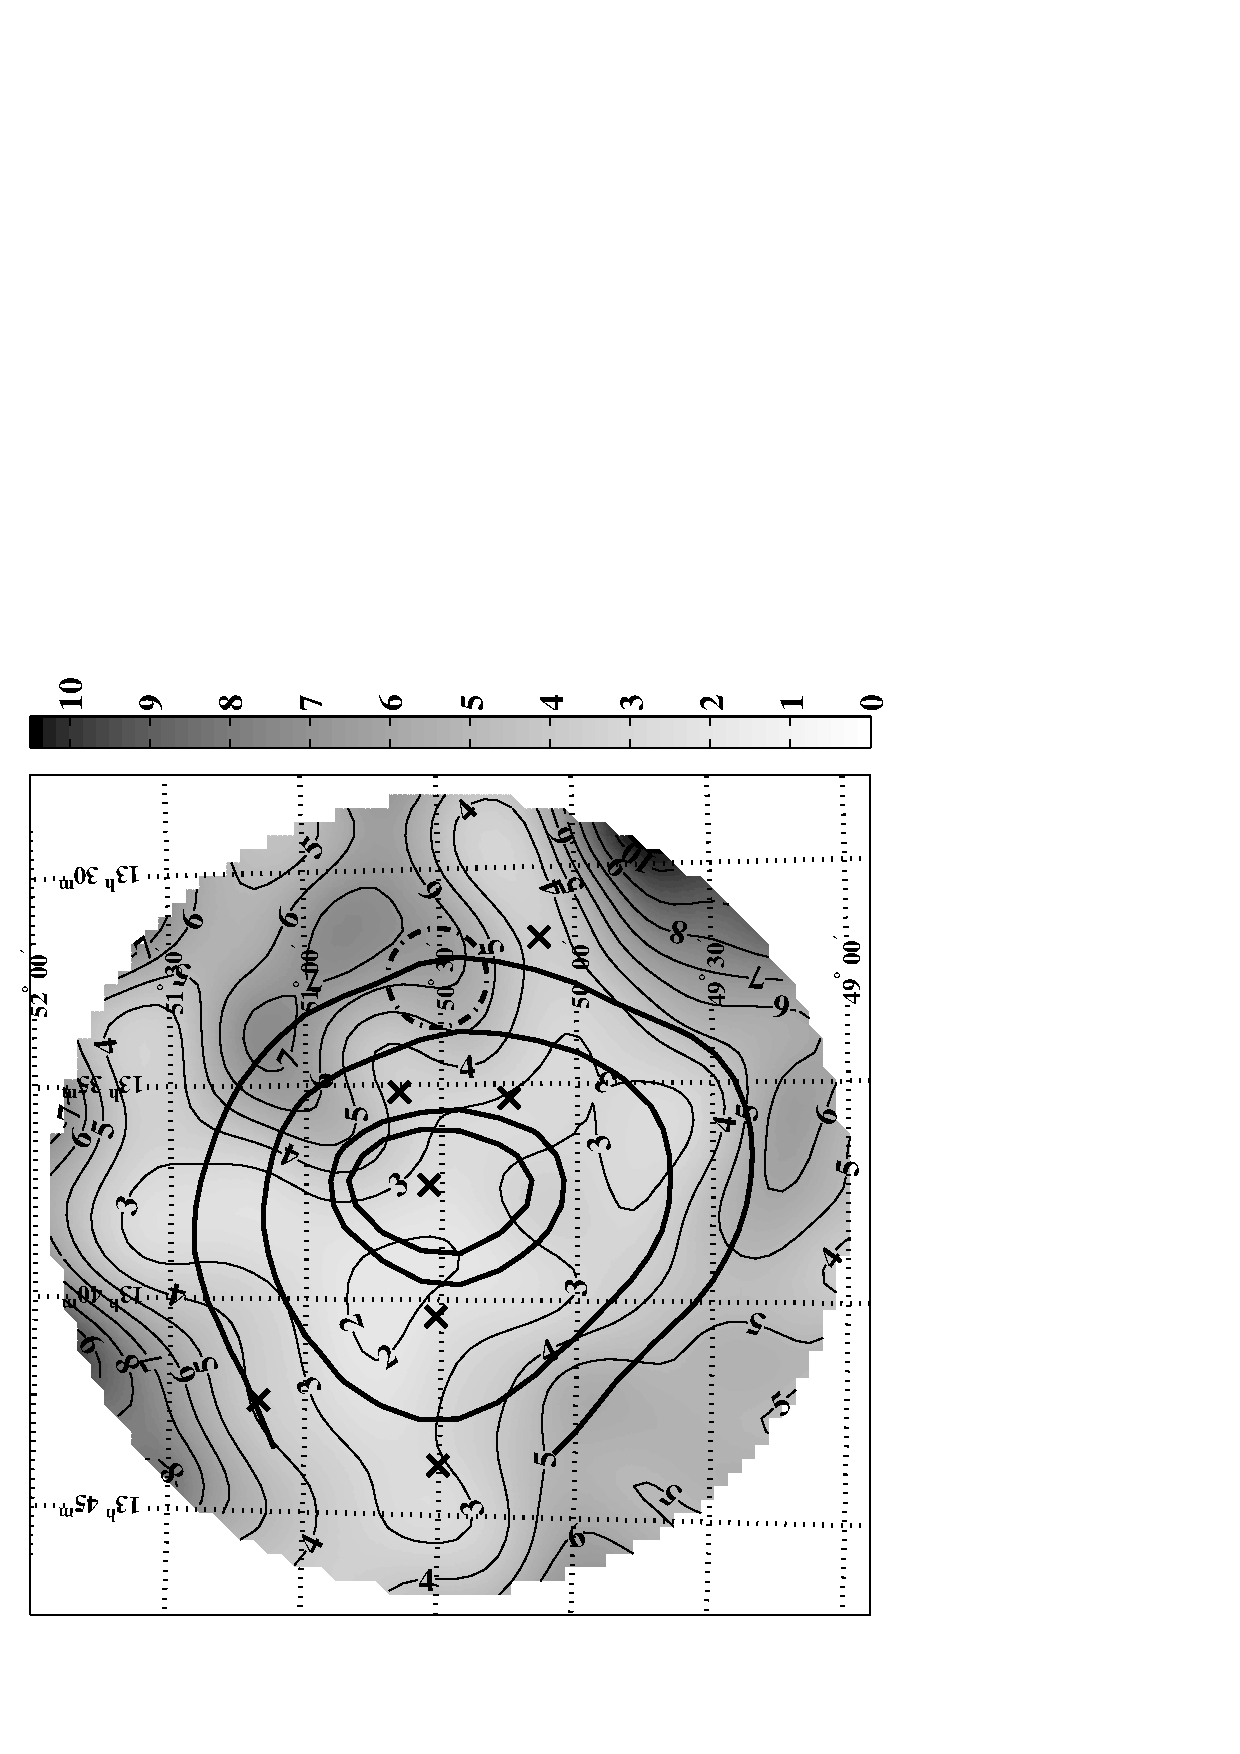
\includegraphics[draft=false,width=\textwidth,angle=270]{plots/chap-observations/loenergy/J1337+5029_sul_conv_bw.pdf}\includegraphics[width=\textwidth,angle=270]{plots/chap-observations/spectra/3EG_J1337+5029.pdf}}
\caption{\label{FIG::OBSERVATIONS::J1337UL} (Left) Limits on 
emission from 3EG J1337$+$5029 in units of
$10^{-11}$\,cm$^{-2}$\,s$^{-1}$. The 3EG error contours are overlaid
as heavy lines. (Right) Spectrum from the on-line version of the 3EG
catalog with the limit at 350\,GeV.}
\end{figure}

Since VHE emission is not claimed, upper limits for the region and
potential associations are presented in
figure~\ref{FIG::OBSERVATIONS::J1337UL} and
table~\ref{TAB::OBSERVATIONS::J1337}. An upper limit of
$F_{(>350\,\mathrm{GeV})}<5.9\times10^{-11}$\,cm$^{-2}$\,s$^{-1}$ is
derived for the EGRET source. 
%This limit is higher than for other sources in the survey due to the 
%small dataset and the large excess of events. 
Figure~\ref{FIG::OBSERVATIONS::J1337UL} (right) shows the upper limit,
which rules out half of the flux space allowed by extrapolating the
EGRET spectrum to 350\,GeV. Upcoming observations will either detect
emission from this source or further constrain its spectrum.

% RASS DATA
%  cos(d)   SrcNam                                              R.A.     Dec       ?p #id catalog_id F             gal_Nh gal_long gal_lat        hr1   ?hr1  hr2   ?hr2 ext exl srcl  exp src-cps  ?src-cps flux1      flux2          t_obs_beg t_obs_end  orgdat moddat
% 0.999902  1RXS J133230.8+502436  RX J1332.5+5024             203.1283  50.4101   19  16 1RXS       x              0.102 107.0738  65.4343       0.70  0.11  0.43  0.11  72  37  44   566 1.49E-01 2.00E-02  1.586E-12 1.797E-12      901204.98 901207.51  960614 000000
% 0.999911  1RXS J133243.3+503256  RX J1332.7+5032  Cluster    203.1804  50.5489   18  27 1RXS       x              0.102 107.1273  65.2934       0.51  0.10  0.10  0.13  75  43  80   564 2.05E-01 2.22E-02  2.179E-12 2.261E-12      901204.91 901207.25  960614 000000
% 0.999974  1RXS J133510.2+503920                   Star/Dwarf 203.7925  50.6556    8   7 1RXS       x              0.102 106.3751  65.0434      -0.30  0.09 -0.22  0.16  10   1 190   562 1.98E-01 2.15E-02  2.101E-12 1.331E-12      901205.31 901207.98  960614 000000
% 0.999973  1RXS J133519.6+501504  RX J1335.3+5015  AGN/Star   203.8317  50.2511    9  12 1RXS       x              0.115 105.9311  65.4034      -0.43  0.13  0.21  0.27   0   0  68   564 9.21E-02 1.55E-02  1.044E-12 5.555E-13      901205.78 901208.18  960614 000000
% 0.999999  1RXS J133720.0+503252  RX J1337.3+5032             204.3333  50.5479    9   5 1RXS       x              0.102 105.5291  65.0010      -0.42  0.14  0.06  0.28   0   0  61   566 7.66E-02 1.37E-02  8.128E-13 4.660E-13      901205.85 901208.58  960614 000000
% 0.999968  1RXS J134023.3+503113                   Star       205.0971  50.5204    8  21 1RXS       x              0.115 104.4681  64.8165      -0.14  0.07 -0.12  0.11  15   4 372   541 3.65E-01 2.87E-02  4.141E-12 2.765E-12      901206.58 901209.25  960614 000000
% 0.999846  1RXS J134350.8+503016                              205.9617  50.5044    9   6 1RXS       x              0.115 103.3066  64.5796      -0.12  0.14  0.23  0.20   0   0  76   520 9.98E-02 1.72E-02  1.131E-12 7.659E-13      901207.31 901209.91  960614 000000

\subsection{3EG~J1826$-$1302 and 3EG~J1823$-$1314}

The low latitude \Gray sources 3EG~J1826$-$1302 and 3EG~J1823$-$1314
are the closest sources to the Galactic center to be studied in this
survey. 3EG~J1826$-$1302 has a relatively hard, well determined
spectrum ($\Gamma=2.00\pm0.11$), a large 100\,MeV flux, and shows
evidence of being variable ($\delta=0.88$ from
\citealt{REF::NOLAN::APJ2003}). 3EG~J1823$-$1314 has a softer spectrum
($\Gamma=2.69\pm0.19$), a large flux and a variability index of
$\delta=0.60$. The center of the sources lie approximately $0.8^\circ$
apart, a separation that is considerably smaller than the EGRET
point-spread function at 100\,MeV; they are listed in the 3EG catalog
as having positions, fluxes and significances that could be affected
by source confusion. Their 99\% confidence contours overlap
considerably, their 95\% contours overlap to a smaller degree. The GeV
catalog lists a source, GeV~J1825$-$1310 which overlaps both of the
3EG sources but is more consistent with being associated with
3EG~J1826$-$1302. Finally, a third EGRET source 3EG~J1824-1514 is also
close to these sources ($\sim2^\circ$) and is partially within
the field of view of the VHE observations, as described below.

\citet{REF::ROBERTS::APJS2001} present x-ray observations of the
\Gray error-box in their catalog of ASCA observations of 
the bright GeV sources. Their image revealed a previously unknown
extended x-ray source, denoted AX~J1826.1$-$1300, which they conclude
is a PWN. The putative PWN is centered on the 3EG source J1826$-$1302,
and makes a good potential counterpart for the \Gray source. A
pulsar/PWN origin would account for the hardness of the EGRET
spectrum, and the variability index of $\delta=0.88$ is consistent
with the value of $0.66\pm0.29$ which \citet{REF::NOLAN::APJ2003}
calculate as the mean for the class of six potential pulsar/PWN
associations suggested by \citet{REF::GRENIER::TEXAS2002}.
\citet{REF::ROBERTS::APJS2001} also report extended emission near the 
non thermal radio source SNR~18.1-0.2, reported as a possible SNR by
\citet{REF::ODEGARD::AJ1986} (but not adopted as such by
\citealt{REF::GREEN::WEB2001}), and remark that it is consistent with
the 100\,MeV source 3EG~J1823$-$1314.

The much studied PSR~B1823$-$13, a young, energetic, Vela-like pulsar,
is contained within the 95\% error contour of 3EG~J1826$-$1302. The
source has been targeted for VHE observations with the Whipple
\citep[see][and its references]{REF::HALL::ICRC2001} and HEGRA
\citep[identified as PSR~J1826-1334]{REF::AHARONIAN::AA2002}
telescopes, with limits of
$F_{(>520\,\mathrm{GeV})}<0.91\times10^{-11}$\,cm$^{-2}$\,s$^{-1}$ and
$F_{(>1700\,\mathrm{GeV})}<0.48\times10^{-11}$\,cm$^{-2}$\,s$^{-1}$
being derived respectively. \citet{REF::GAENSLER::APJ2003} present
deep XMM-Newton observations of the pulsar, in which they discover two
components of emission, a core of hard x-ray emission of 5\,arcsec
extent surrounded by an asymmetric region of fainter, softer, diffuse
emission toward the south of the pulsar. They do not detect the radio
pulsar, either as a compact point source or through pulsations. No
associated SNR is seen.

\begin{figure}[p]
\centerline{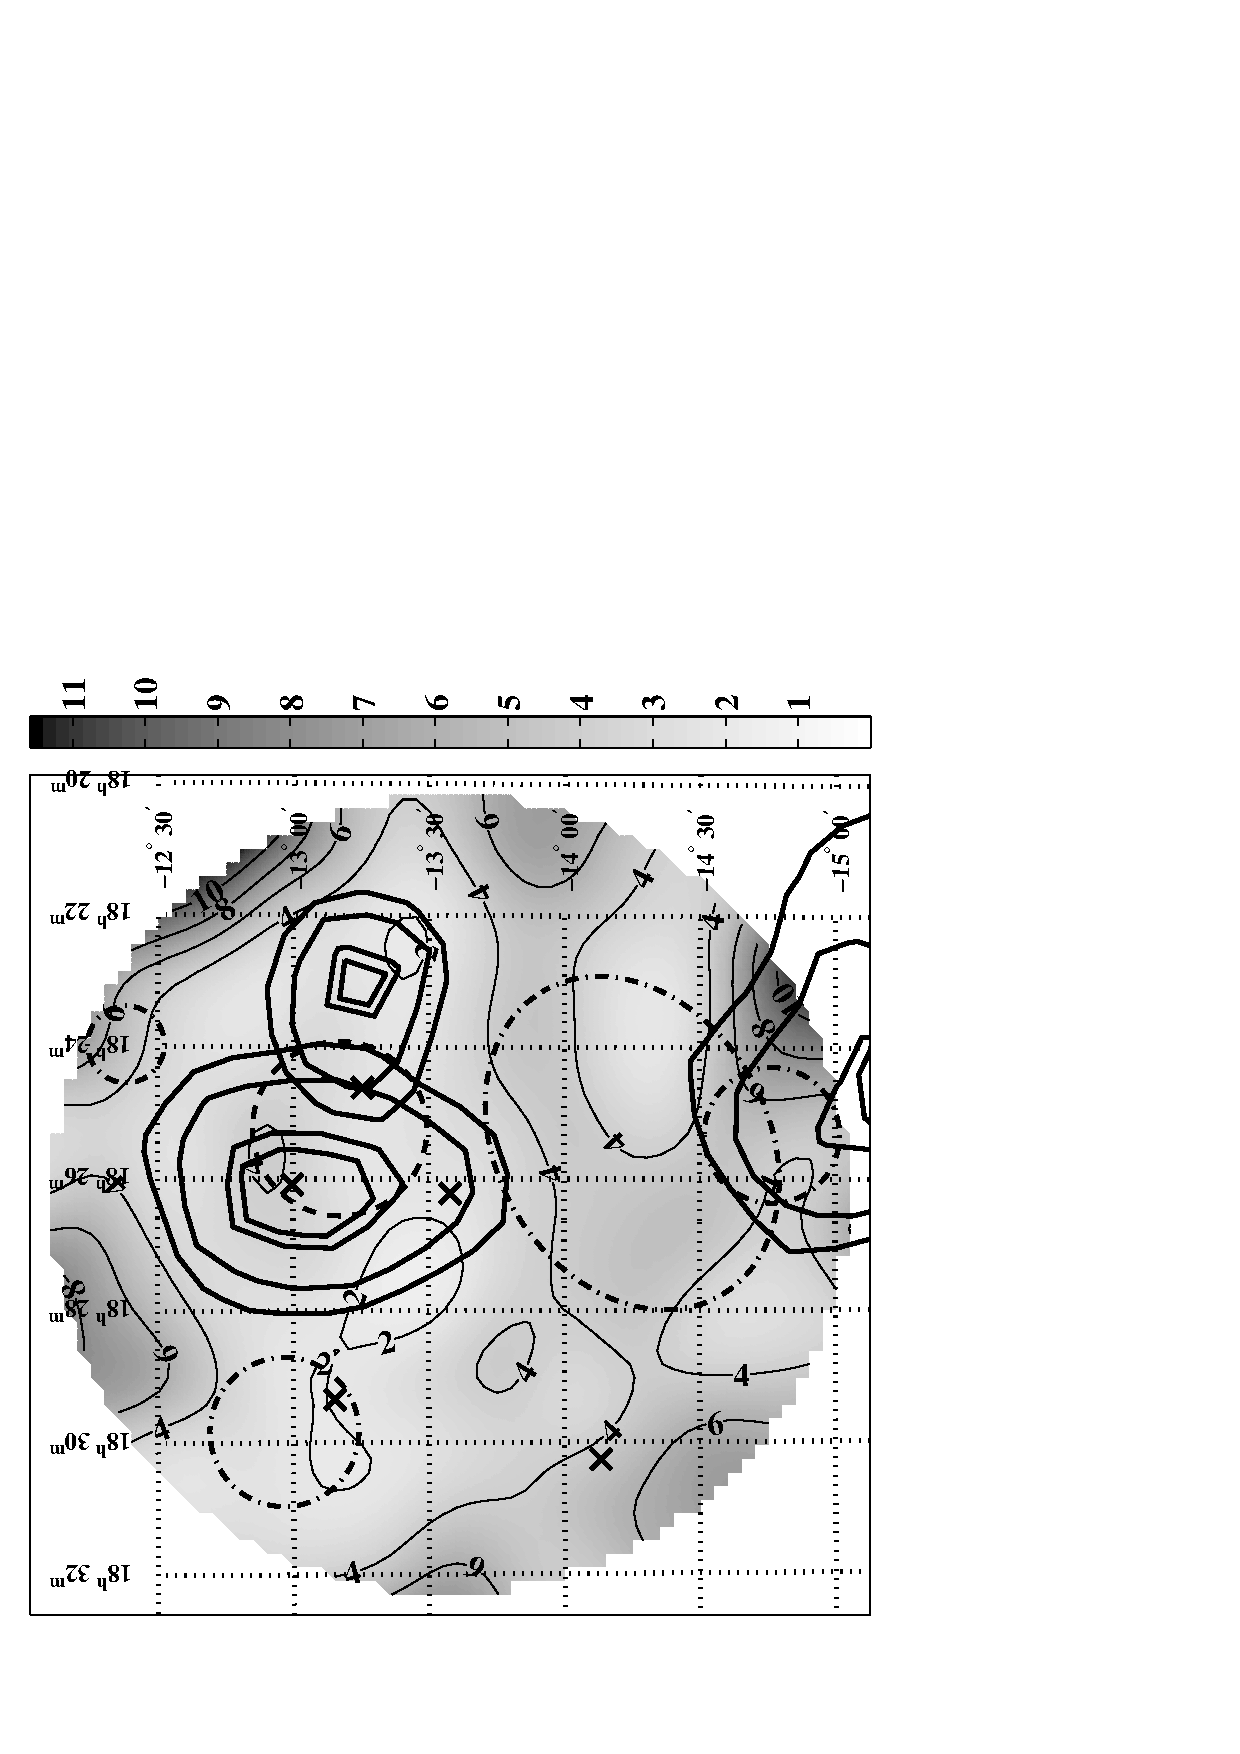
\includegraphics[draft=false,angle=270,width=0.8\textwidth]{plots/chap-observations/loenergy/J1826-1302_sul_conv_bw.pdf}}
\centerline{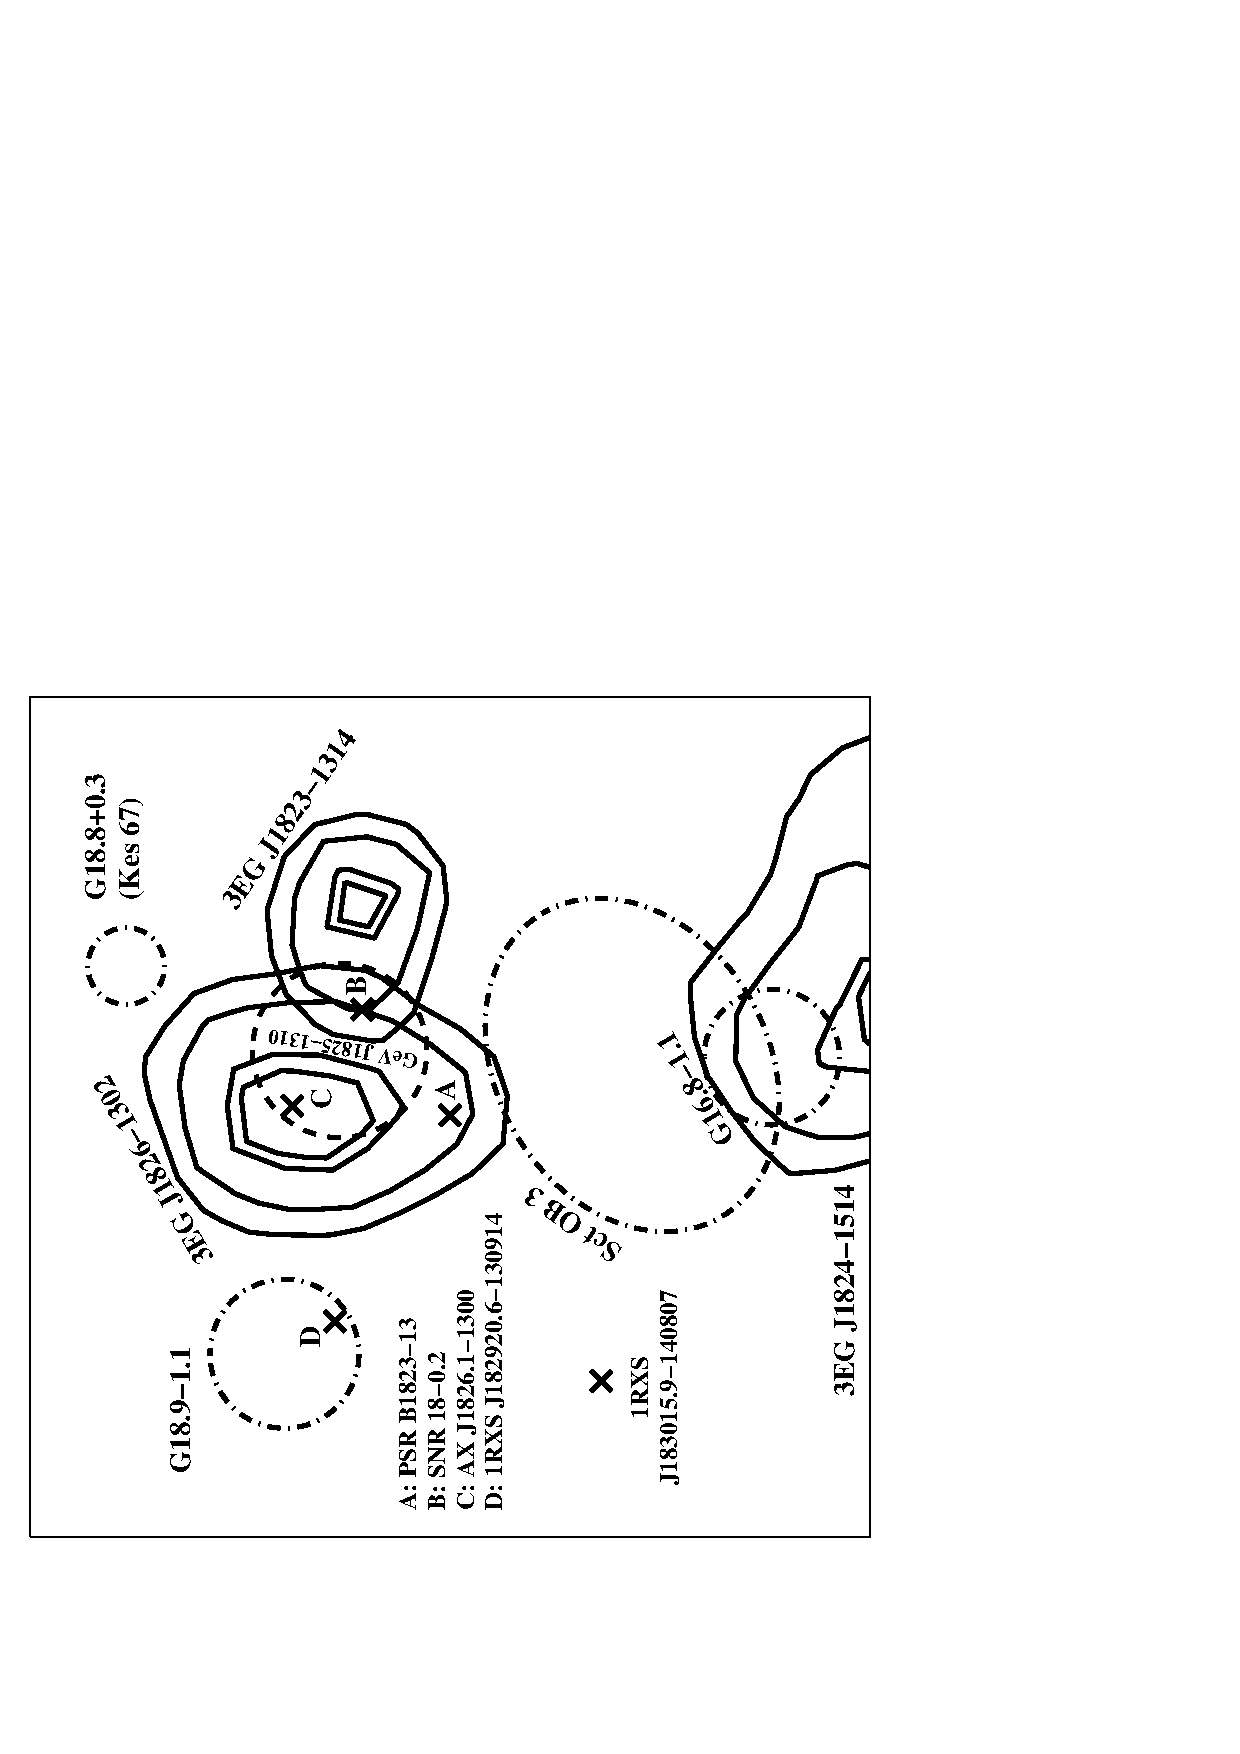
\includegraphics[angle=270,width=0.5\textwidth]{plots/chap-observations/loenergy/J1826-1302_guide_bw.pdf}}
\caption{\label{FIG::OBSERVATIONS::J1826UL} Upper limits on emission 
from 3EG~J1826$-$1302, 3EG~J1826$-$1302 and GeV~J1825$-$1310 in units
of $10^{-11}$\,cm$^{-2}$\,s$^{-1}$. The SNR, OB association and
point source candidates in the field are indicated on the figure
and labeled in the key below, as is a third EGRET source
3EG~J1824$-$1514 which partially overlaps the field.}
\end{figure}

\begin{table}[p]
\caption{\label{TAB::OBSERVATIONS::J1826} Upper limits for candidates
in 3EG~J1826$-$1302 field.}
\centerline{\begin{tabular}{lllll}\hline
Source Name & \multicolumn{2}{l}{Coordinates} & Extent & Upper Limit \\
& $\alpha_{2000}$  & $\delta_{2000}$ & deg & $\times10^{-11}$\,cm$^{-2}$\,s$^{-1}$\\\hline
3EG~J1826$-$1302        & $18^h26^m01.0^s$ & $-13^\circ05^{\prime}28^{\prime\prime}$ & $0.55\times0.39$ & 4.2 \\
3EG~J1823$-$1314        & $18^h23^m24.7^s$ & $-13^\circ14^{\prime}32^{\prime\prime}$ & $0.33\times0.23$ & 3.2 \\
GeV~J1825$-$1310        & $18^h25^m14.3^s$ & $-13^\circ10^{\prime}19^{\prime\prime}$ & $0.32\times0.32$ & 4.2 \\
PSR~B1823$-$13          & $18^h26^m13.2^s$ & $-13^\circ34^{\prime}47^{\prime\prime}$ & -                & 2.4 \\
SNR~18.1$-$0.2          & $18^h24^m37.0^s$ & $-13^\circ15^{\prime}18^{\prime\prime}$ & $0.03\times0.01$ & 2.6 \\
AX~J1826.1$-$1300       & $18^h26^m04.9^s$ & $-12^\circ59^{\prime}48^{\prime\prime}$ & -                & 3.7 \\
G16.8$-$1.1             & $18^h25^m20.0^s$ & $-14^\circ46^{\prime}00^{\prime\prime}$ & $0.25\times0.25$ & 6.9 \\
G18.8$-$0.3 (Kes~67)    & $18^h23^m58.0^s$ & $-12^\circ23^{\prime}00^{\prime\prime}$ & $0.14\times0.14$ & 6.8 \\
G18.9$-$1.1             & $18^h29^m50.0^s$ & $-12^\circ58^{\prime}00^{\prime\prime}$ & $0.28\times0.28$ & 3.6 \\
Sct~OB~3                & $18^h25^m27.2^s$ & $-14^\circ15^{\prime}04^{\prime\prime}$ & $1.30\times1.00$ & 6.2 \\
$^*$J183015.9-140807    & $18^h30^m15.9^s$ & $-14^\circ08^{\prime}07^{\prime\prime}$ & -                & 4.6 \\
$^*$J182920.6-130914    & $18^h29^m20.6^s$ & $-13^\circ09^{\prime}14^{\prime\prime}$ & -                & 2.0 \\\hline
\end{tabular}}
\centerline{\footnotesize{\begin{tabular}{p{0.9\textwidth}}
$^*$ The standard RASS-BSC catalog prefix of 1RXS is omitted for formatting purposes.\\
\end{tabular}}}
\end{table}

\begin{figure}[p]
\includegraphics[angle=270,width=0.49\textwidth]{plots/chap-observations/spectra/3EG_J1826-1302.pdf}\hspace*{\fill}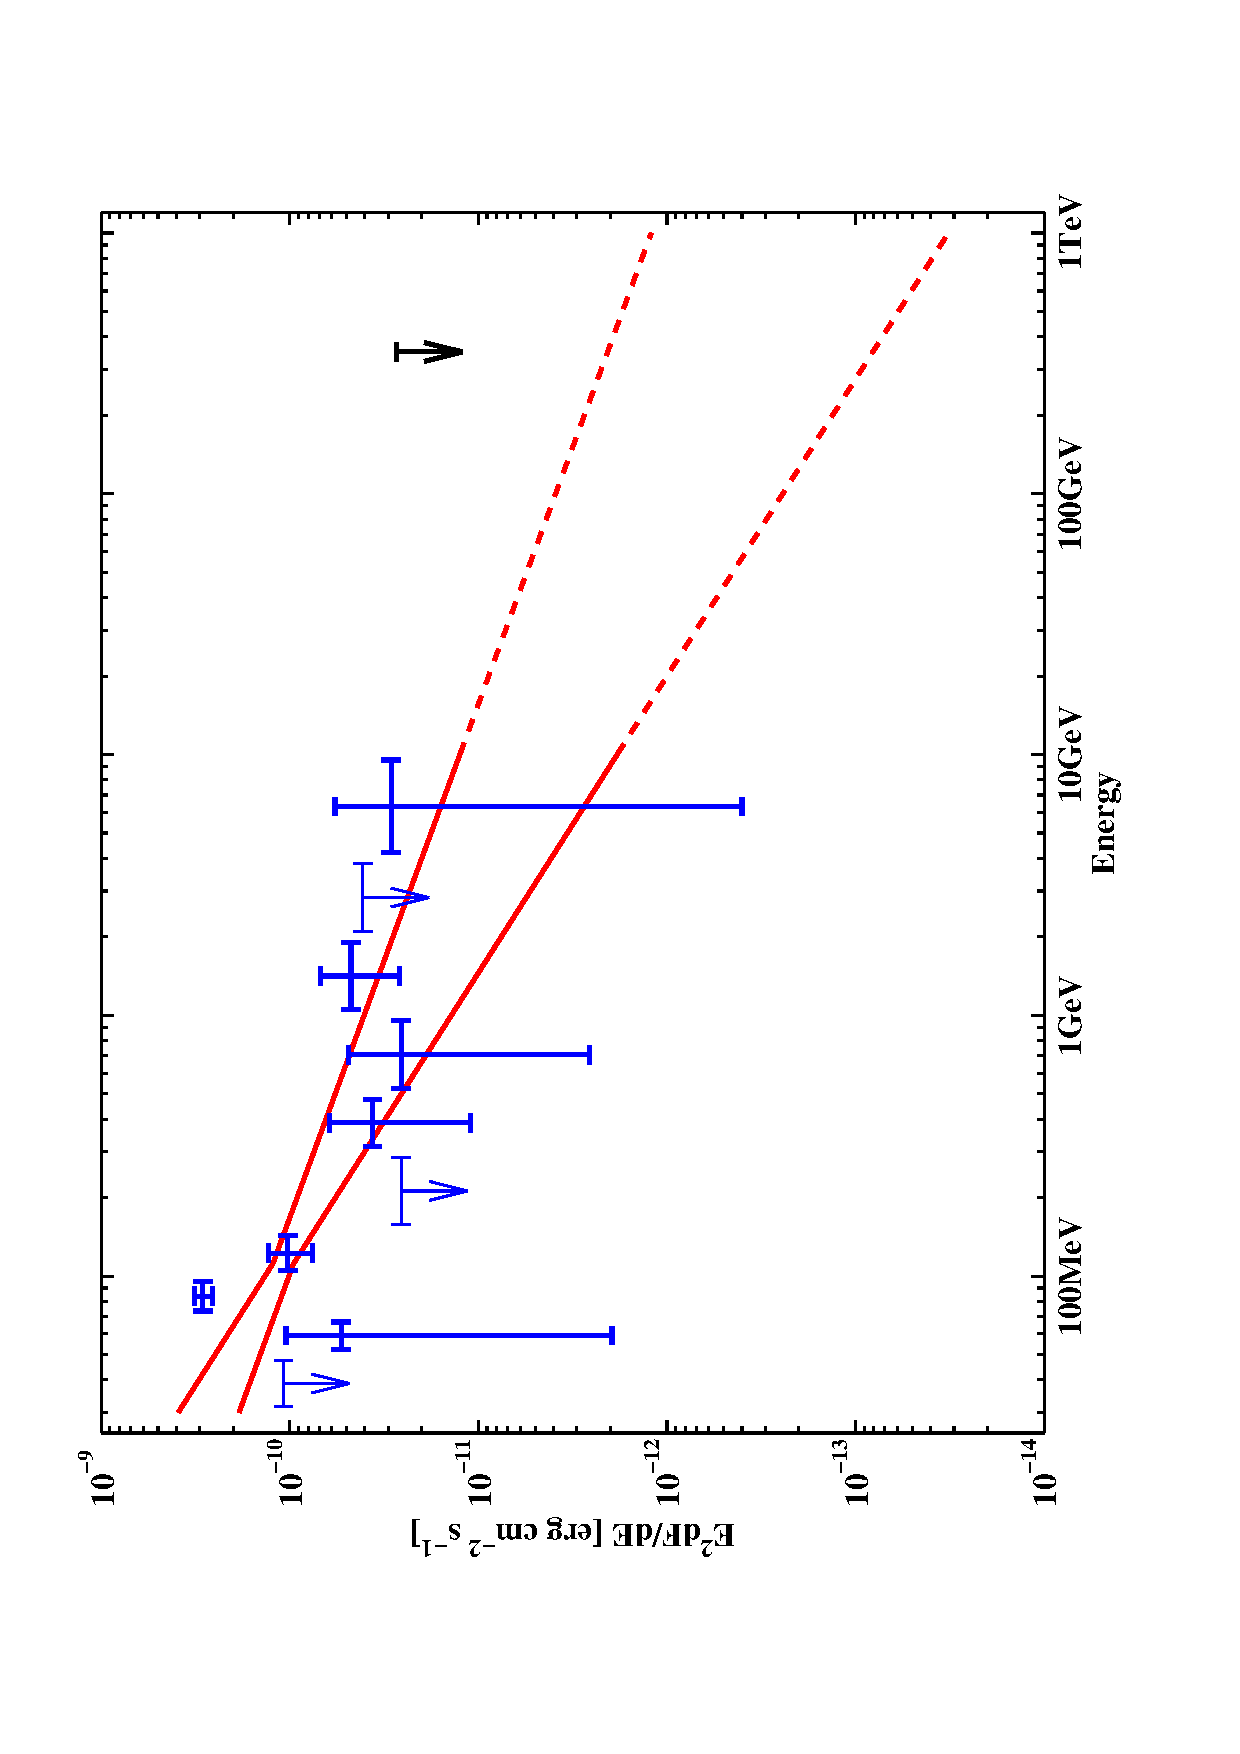
\includegraphics[angle=270,width=0.49\textwidth]{plots/chap-observations/spectra/3EG_J1823-1314.pdf}
\caption{\label{FIG::OBSERVATIONS::J1826SPEC} Spectrum for 
3EG~J1826$-$1302 (left) and 3EG~J1823$-$1314 (right) from on-line
version of the 3EG catalog with the upper limit at 350\,GeV.}
\end{figure}

\citet{REF::GREEN::WEB2001} contains three SNR within the field of
view of the VHE observations, one of which, G18.8$-$0.3 (or Kes~67),
was suggested by \citet{REF::STURNER_DERMER::AA1995} as a candidate
for a source in the first EGRET catalog (GRO~1923$-$12 from
\citealt{REF::FICHTEL::APJS1994}). None of the SNR are within
the 95\% confidence contours of the two EGRET sources reported on
here. \citet{REF::ROMERO::AA1999} lists a positional coincidence
between the three EGRET sources in the field and the OB association
Sct~OB~3. The association does not significantly overlap
3EG~J1826$-$1302 or 3EG~J1823$-$1314 but does show some overlap with
3EG~J1826$-$1302 and with the SNR~G16.8$-$11. Previous VHE limits for
the three SNR (and for many other Galactic SNR) have been presented by
the HEGRA collaboration \citep{REF::AHARONIAN::AA2002}.
\citet{REF::MATTOX::APJS2001} do not have potential
radio candidates for these 3EG sources. The RASS-BSC contains two
x-ray sources, listed in table~\ref{TAB::OBSERVATIONS::J1826}, in the
field.

Clearly, the source region is dense with potential counterparts. It is
also possible that the correct association for the sources has not yet
been resolved at other energies, e.g.\ the SNR counterparts for
PSR~B1823$-$13 and for AX~J1826$-$1300 have not been identified, this
could be the case for other SNR in the field. 

The VHE observations of these sources were made as part of a search
for emission from the pulsar, consequently the field is centered on
PSR~B1823$-$13. A total of 416\,min.\ of data were collected between
April and July 2000. The results of a point source analysis of the
data have been previously published in \citet{REF::HALL::ICRC2001,
REF::HALL::ICRC2003}. The two dimensional analysis did not reveal any
significant emission. Upper limits for the region and various
potential associations are presented in
figure~\ref{FIG::OBSERVATIONS::J1826UL}, which includes a key to the
complex field, and summarized in table~\ref{TAB::OBSERVATIONS::J1826}.
A limit of
$F_{(>350\,\mathrm{GeV})}<4.2\times10^{-11}$\,cm$^{-2}$\,s$^{-1}$ is
derived for the hard \Gray source 3EG~J1826$-$1302. A somewhat lower
limit of
$F_{(>350\,\mathrm{GeV})}<3.2\times10^{-11}$\,cm$^{-2}$\,s$^{-1}$ is
derived for the smaller, softer 3EG~J1823$-$1314.

The VHE upper limits are displayed in
figure~\ref{FIG::OBSERVATIONS::J1826SPEC} with an extrapolation of the
EGRET spectrum. The limit derived for the region of 3EG~J1826$-$1302
constrains the hard EGRET spectrum to the softest spectrum allowed by
the errors in the 100\,MeV flux and spectral index. It is likely that
a cutoff in the spectrum occurs between the highest EGRET flux point,
at 6\,GeV, and the VHE observations. In the case of 3EG~J1823$-$1314,
the softer EGRET spectrum is not constrained by the VHE upper limit.

\subsection{3EG~J1835$+$5918}

The bright \Gray source 3EG~J1835$+$5918 has the hardest spectral
index and smallest error circle among all of the EGRET sources
classified as unidentified. The source was detected consistently
throughout the EGRET mission; \citet{REF::NOLAN::APJ2003} calculate a
variability index of $\delta=0.15$. The hard spectrum and low
variability suggest an association with a pulsar, although none have
been definitively identified in the field.

The source has been extensively studied at radio, optical and x-ray
energies by two independent groups \citep[see][and references
therein]{REF::REIMER::NSPS2002, REF::HALPERN::APJ2002}, who present
compelling evidence that the source is associated with an isolated
neutron star, possibly a radio-quiet, Geminga-like pulsar. Taking just
one of these groups' work (Halpern et al.):
\citet{REF::MIRABAL::APJ2000} report on a series of observations with
many different instruments across the spectrum, which narrowed the
list of potential ROSAT and ASCA x-ray candidate associations in the
95\% error contour from ten to one: RX~J1836.2$+$5925. Optical/UV
photometry uncovered 40 possible AGN in the field, based on a search
for broad UV continuum emission. Twenty radio sources were found in
archival VLA observations or standard radio catalogs. In particular,
no flat-spectrum radio sources, which could correspond to FSRQs and
BL~Lacs, the only AGN identified as EGRET sources to date, were
identified in the field. Follow-up optical spectra of the candidates
revealed that most of the x-ray sources were distant AGN or G- to
M-type stars. Only RX~J1836.2$+$5925, the brightest of the ROSAT
sources, was unidentified in the initial optical survey, and was
selected as the mostly likely counterpart for the
\Gray source, although its properties were unlike any other known
EGRET source. \citet{REF::MIRABAL::APJ2001} report a reanalysis of the
ROSAT data in which soft x-ray emission below 0.4\,keV became
apparent, which they conclude is thermal emission from the surface of
an isolated neutron star. Subsequent observations with the Chandra
x-ray satellite and Hubble space telescope
\citep{REF::HALPERN::APJ2002} make this conclusion very compelling, the
excellent resolution of the Chandra instrument rules out all possible
optical counterparts in the HST image, down to the limiting magnitude
of $V>28.5$.  These observations make an association with an AGN very
unlikely and constrain the distance and temperature of a neutron star
(NS) candidate.  They conclude that it must have temperature of
$T\approx3\times10^5$\,K, be very distant (compared with the Geminga
pulsar), $d\approx800$\,pc. Given a standard model for NS cooling,
they calculate an age of $\sim10^6$\,yr. No SNR was detected around
the pulsar in sensitive VLA observations, it seems likely that the NS
was ejected from the remnant at birth and traveled to its present
location.  If the NS started in (or near) the Galactic plane and the
putative distance of 800\,pc is correct, the NS must have traveled a
distance of 340\,pc to reach its present location (latitude of
$b=25^\circ$); \citet{REF::HALPERN::APJ2002} conclude this is not
unreasonable, given its age of one million years.

VHE observations of this source during May and June 2000 resulted in
110\,min.\ of data, pointed at the center of the 3EG source. The data
were analyzed with the two dimensional technique and no statistically
significant emission was detected. Limits for the region are presented
in figure~\ref{FIG::OBSERVATIONS::J1835} and summarized in
table~\ref{TAB::OBSERVATIONS::J1835}. A limit of
$F_{(>350\,\mathrm{GeV})}<3.8\times10^{-11}$\,cm$^{-2}$\,s$^{-1}$ is
derived for the field, which clearly constrains an extrapolation of
the EGRET spectrum to the VHE regime (see
figure~\ref{FIG::OBSERVATIONS::J1835}). A cutoff is required in the
spectrum between the highest EGRET energies and 350\,GeV, supporting
the case for a pulsar origin of the {\Grayc}s.
\citet{REF::HALPERN::APJ2002} suggest that this cutoff is visible in the
4\,GeV EGRET point, which is considerably below the expected power law
flux, although the deficit may also be the result of low photon
statistics.

\begin{figure}[t]
\resizebox*{\textwidth}{!}{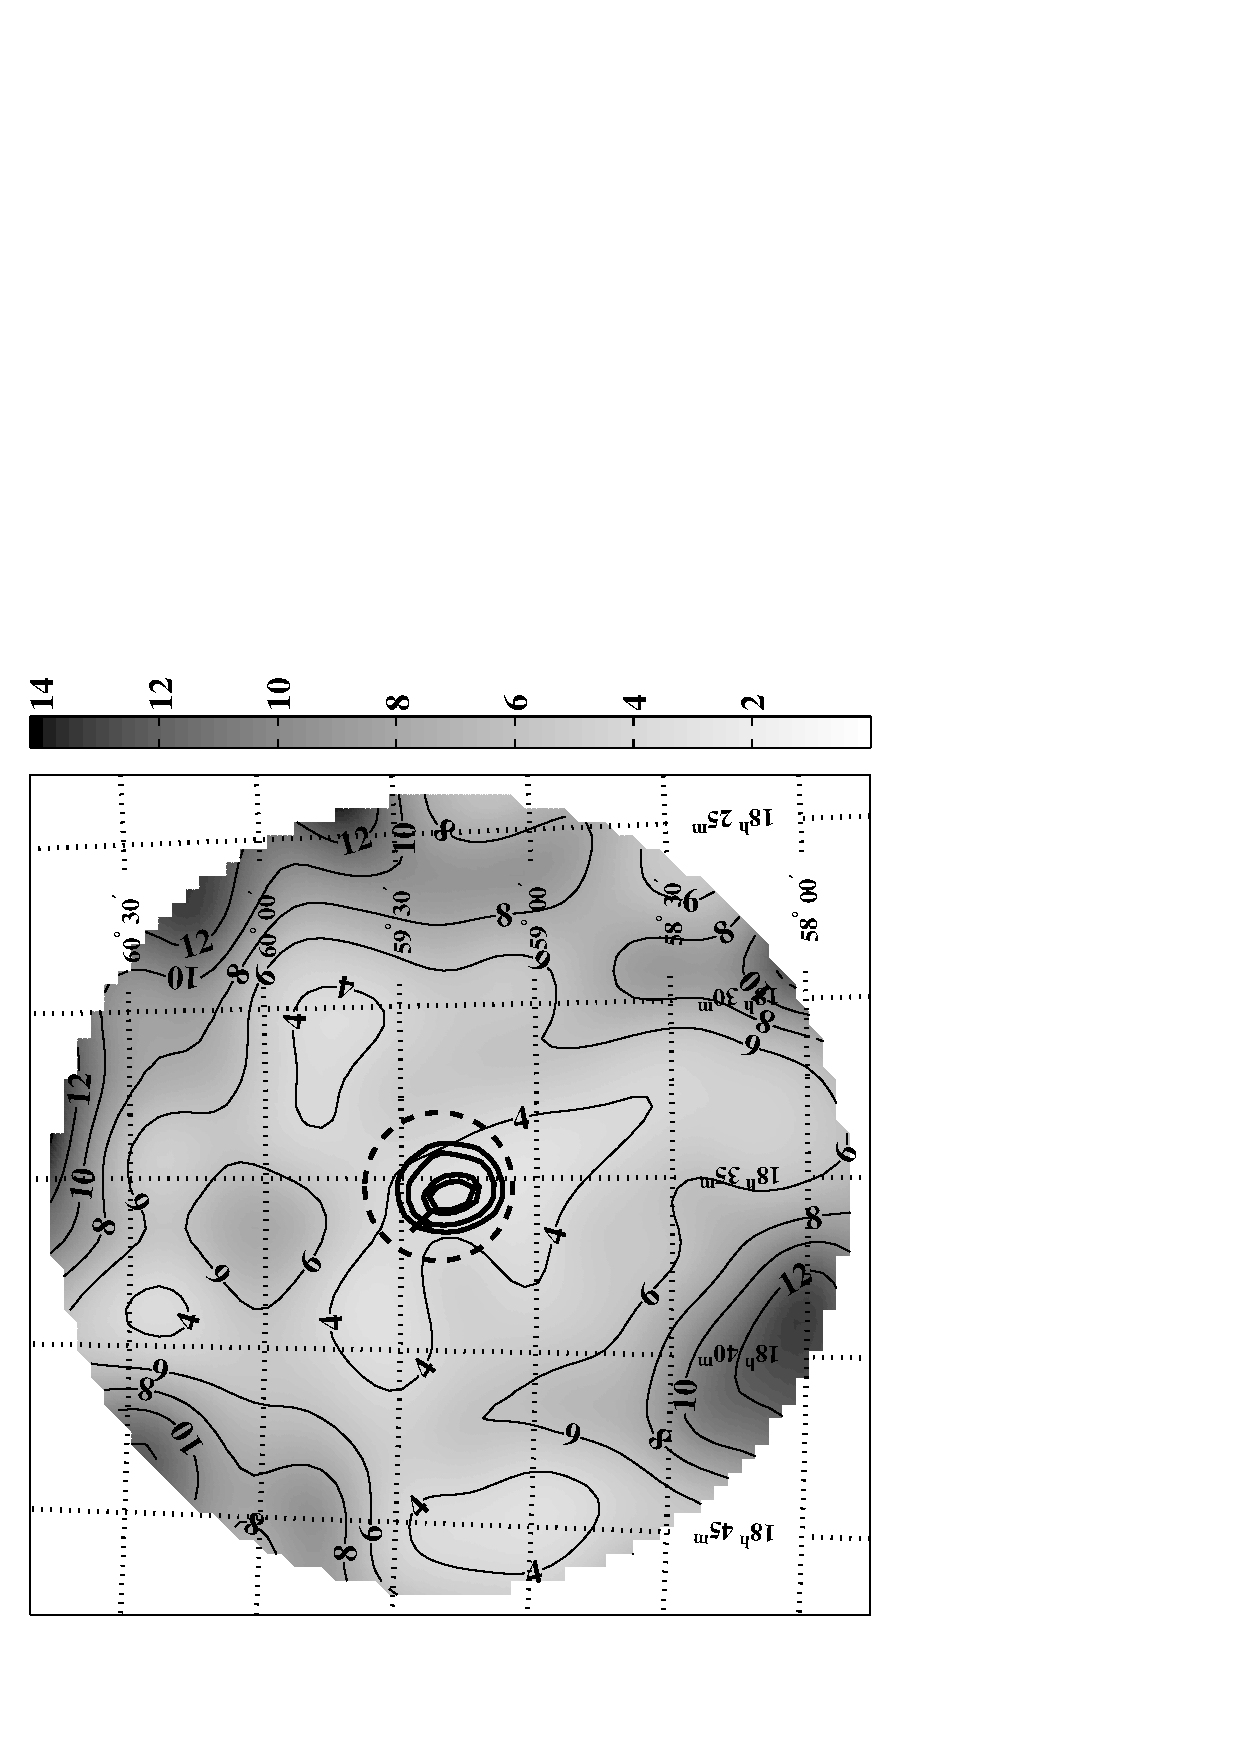
\includegraphics[draft=false,width=\textwidth,angle=270]{plots/chap-observations/loenergy/J1835+5918_sul_conv_bw.pdf}\includegraphics[width=\textwidth,angle=270]{plots/chap-observations/spectra/3EG_J1835+5918.pdf}}
\caption{\label{FIG::OBSERVATIONS::J1835} (Left) Limits on emission from 
3EG J1835$+$5918 in units of $10^{-11}$\,cm$^{-2}$\,s$^{-1}$. The 3EG
error contours are overlaid as heavy lines. (Right) Spectrum from
the on-line version of 3EG catalog with the limit at 350\,GeV.}
\end{figure}

\begin{table}[t]
\caption{\label{TAB::OBSERVATIONS::J1835} Upper limits for candidates
in 3EG~J1835$+$5918 field.}
\centerline{\begin{tabular}{lllll}\hline
Source Name & \multicolumn{2}{l}{Coordinates} & Extent & Upper Limit \\
& $\alpha_{2000}$ & $\delta_{2000}$ & deg & $\times10^{-11}$\,cm$^{-2}$\,s$^{-1}$\\\hline
3EG~J1835$+$5918     & $18^h35^m24.9^s$ & $+59^\circ19^{\prime}15.3^{\prime\prime}$ & $0.16\times0.13$ & 3.8 \\
RX~J1836.2$+$5925    & $18^h36^m13.7^s$'& $+59^\circ25^{\prime}30.1^{\prime\prime}$ & -                & 3.7 \\\hline
\end{tabular}}
\end{table}

\subsection{GeV~J1907$+$0557}

The GeV source J1907$+$0557 does not have a counterpart 100\,MeV EGRET
source, although 3EG~J1903$+$0550 is listed incorrectly in the 3EG
catalog as being associated with it; there is very little overlap at
the 95\% confidence level. \citet{REF::STURNER_DERMER::AA1995} suggest
that a first EGRET catalog source in the region is associated with the
SNR G40.5$-$0.5; an association of the SNR with the revised positions
of the GeV and 3EG sources seems unlikely.  There are two additional
SNR in the region listed by \citet{REF::GREEN::WEB2001}, neither is a
likely counterpart for the GeV source. One of them (G39.2$-$0.3) is
listed by \citet{REF::TORRES::PR2003} as a counterpart to the 3EG
source. \citet{REF::ROBERTS::APJS2001} present an ASCA image of the
GeV source in which they discover an extended x-ray source,
AX~J1907.4$+$0557. No other x-ray source appears in the ASCA image,
which covers approximately half of the region within the GeV 95\%
contour.

The center of the GeV source was observed with the Whipple instrument
for 277\,min.\ between May and June 2000. The data shows a large
excess of {\Grayc}-like events whose reconstructed origins are
distributed across the \On\ source region, from the center of the
field to a distance of $>1.8^\circ$ from the center, by which point
the number of events drops quickly due to the limited field of view of
the instrument. It is unlikely that such a broad excess is the result
of \Gray emission from a large, extended source; rather it is likely
to be the result of a difference in brightness between the \On\ and
\Off\ source regions which is not completely compensated for by the
data selection algorithm. In order to remove this systematic effect,
the number of events in an annulus defined by
$1.4^\circ<dist<1.8^\circ$ is calculated from the \On-source and
\Off-source data and their ratio used to scale number of \Off-source
counts to the \On-source region. After this rescaling, no significant
excess or deficit is present, upper limits on \Gray emission are
presented in figure~\ref{FIG::OBSERVATIONS::J1907UL} and summarized in
table~\ref{TAB::OBSERVATIONS::J1907}. A limit of
$F_{(>350\,\mathrm{GeV})}<3.0\times10^{-11}$\,cm$^{-2}$\,s$^{-1}$ is
placed on emission from within the GeV error circle. A limit cannot be
placed on VHE emission from the 3EG source, since it is not fully
contained within the field of view. No spectral information is
available for this object at EGRET energies, therefore an extrapolated
spectrum is not shown. 

\begin{figure}[p]
\centerline{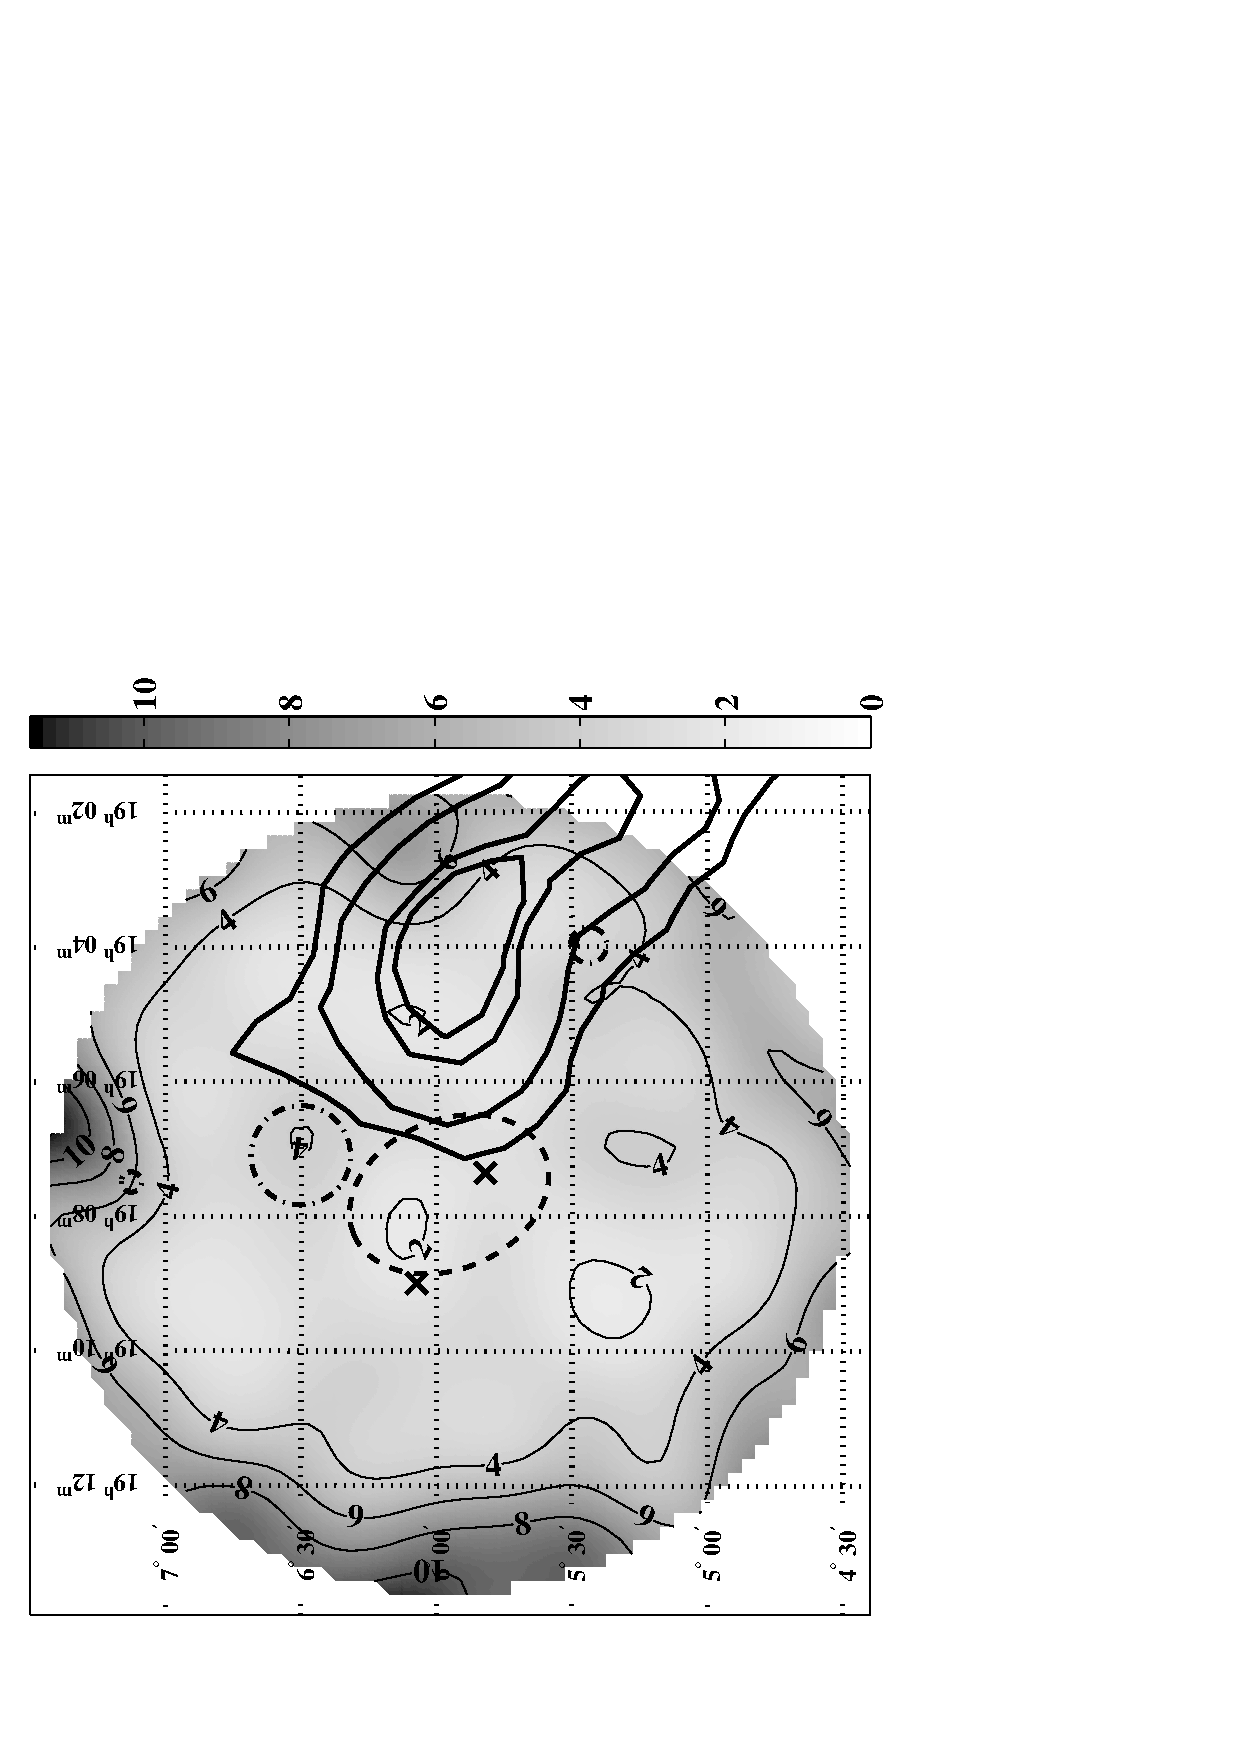
\includegraphics[draft=false,angle=270,width=0.75\textwidth]{plots/chap-observations/loenergy/J1907+0557_sul_conv_bw.pdf}}
\caption{\label{FIG::OBSERVATIONS::J1907UL} Limits on emission 
from GeV~J1907$+$0557 in units of $10^{-11}$\,cm$^{-2}$\,s$^{-1}$. The
GeV error ellipse is shown as a dashed line.  The dash-dotted
circles correspond to SNR in the field, the heavy ``X'-marks indicate
the x-ray sources from ASCA and ROSAT. The confidence contours of
3EG~J1903$+$0550 partially overlap the field to the west of the GeV
source.}
\end{figure}

\begin{table}[p]
\caption{\label{TAB::OBSERVATIONS::J1907} Upper limits for candidates
in GeV~J1907$+$0557 field.}
\centerline{\begin{tabular}{lllll}\hline
Source Name & \multicolumn{2}{l}{Coordinates} & Extent & Upper Limit \\
& $\alpha_{2000}$ & $\delta_{2000}$ & deg & $\times10^{-11}$\,cm$^{-2}$\,s$^{-1}$\\\hline
GeV~J1907$+$0557       & $19^h07^m40.4^s$ & $+05^\circ57^{\prime}14^{\prime\prime}$ & $0.38\times0.28$ & 3.0 \\
AX~J1907.1$+$0549      & $19^h07^m21.3^s$'& $+05^\circ49^{\prime}14^{\prime\prime}$ & -                & 2.6 \\
G39.2$-$0.3            & $19^h03^m58.7^s$ & $+05^\circ26^{\prime}19^{\prime\prime}$ & $0.07\times0.07$ & 3.6 \\
G40.5$-$0.5            & $19^h07^m05.6^s$ & $+06^\circ30^{\prime}06^{\prime\prime}$ & $0.18\times0.18$ & 4.0 \\
G41.1$-$0.3            & $19^h07^m29.4^s$ & $+07^\circ07^{\prime}35^{\prime\prime}$ & $0.04\times0.04$ & 6.3 \\
$^*$J190859.7$+$060426 & $19^h08^m59.7^s$ & $+06^\circ04^{\prime}26^{\prime\prime}$ & -                & 2,3 \\\hline
\end{tabular}}
\centerline{\footnotesize{\begin{tabular}{p{0.9\textwidth}}
$^*$ The standard RASS-BSC catalog prefix of 1RXS is omitted for formatting purposes.\\
\end{tabular}}}
\end{table}

A limit on VHE emission has been obtained by the HEGRA group
\citep{REF::ROWELL::ICRC2003}; based on an exposure of
$\sim1725$\,min.\ they derive a limit of
$F_{(>700\,\mathrm{GeV})}<0.03\times10^{-11}$\,cm$^{-2}$\,s$^{-1}$,
for emission from the GeV source, approximately 35 times lower than the
limit presented here for an energy threshold that is twice as high
(assuming a standard $\Gamma=2.5$ spectrum). The lower limit is partly
due to the longer exposure, but is also the result of the
multi-telescope technique which enhances background rejection and
allows the \Gray origin to be reconstructed more accurately, which
decreases the amount of smoothing that is required, reducing the
number of background events in each bin of the map, and hence allowing
a stronger upper limit to be derived.

\subsection{GeV~J2020$+$3658 (3EG~J2021$+$3716 and 3EG~J2016$+$3657)}

The first two catalogs of EGRET point sources listed a \Gray source in
the region of the field of the COS-B source 2CG~075$+$00. Further data
resolved two separate sources, 3EG~J2021$+$3716 and 3EG~J2016$+$3657,
each with a spectrum of $\sim2.0$. The GeV catalog also lists a
source in the region, GeV~J2020$+$3658, which is suggested in the 3EG
catalog as a counterpart for
3EG~J2016$+$3657. \citet{REF::ROBERTS::APJS2001} note that this
association is probably incorrect, and that the GeV source is more
likely to be associated with 3EG~J2021$+$3716, with which it has
considerable overlap. Of the two 3EG sources, J2021$+$3716, has a
larger 100\,MeV flux
($F=59.1\pm6.2\times10^{-8}$\,cm$^{-2}$\,s$^{-1}$), harder spectrum
($\Gamma=1.86\pm0.10$) and lower variability index
($\delta=0.36$). The other has a flux of
$34.7\pm5.7$\,cm$^{-2}$\,s$^{-1}$, spectral index of $2.09\pm0.11$
and shows more evidence of variability, with $\delta=0.44$.

An ASCA image of the GeV source region revealed two bright x-ray
sources, one a corresponding to a massive Wolf Rayet binary star
system with a 21.6 day periodicity (WR~141), whose x-ray emission is
consistent with a thermal spectrum at $kT\sim5keV$
\citep{REF::ROBERTS::APJS2001}. The second, identified as
AX~J2021.1$+$3651 was seen to have a non-thermal spectrum; subsequent
investigations with the Arecibo radio receiver revealed a young,
energetic pulsar with period of 104\,ms \citep{REF::ROBERTS::APJ2002}.
The ASCA image also reveals extended x-ray emission, which may be
thermal emission from an SNR or a nearby massive star. The pulsar is
an intriguing candidate for the \Gray source, especially in light of
the hard 3EG spectrum and relatively low variability of the source.
The pulsar is located well within the 95\% confidence region of the
GeV source; its positional association with the 3EG source is less
clear, it lies just outside of the 99\% contour. If the 3EG and GeV
sources correspond to the same object, the WR star system is a better
positional association, although it is not contained within the 95\%
contour of the 3EG source. Finally, a second WR-type star, WR~142 is
located north of the 3EG catalog position, well within the 95\%
region. Source confusion between the adjacent EGRET sources probably
means that there are systematic errors in the positions of the
confidence contours for both 3EG sources and the GeV source; none of
the above candidates should be considered as ruled out based on their
position alone. \citet{REF::ROBERTS::APJ2002} conclude that the pulsar
is the most conservative association, being a member of the only class
of Galactic \Gray sources to be unambiguously identified to date.

\citet{REF::MUKHERJEE::APJ2000} and \citet{REF::HALPERN::APJ2001::2016}
present detailed multiwavelength observations of 19 x-ray sources from
the ROSAT faint source catalog consistent with 3EG~J2016$+$3657. Most
have stellar associations: WR-type systems, binaries, cataclysmic
variables\footnote{A binary system with a white dwarf and red dwarf in
a close orbit of less than 1 solar radius which has an accretion disk
an/or magnetically restricted flow of matter onto the white dwarf.
Some undergo novae events, thermonuclear runaway in their accretion
disks during which the luminosity can increase by factors of 10$^6$.} 
and O- and B-type stars that are members of the OB association
Cyg~OB~1. These candidates are generally dismissed by
\citet{REF::HALPERN::APJ2001::2016}. Two ROSAT sources appear to
be plausible candidates for the \Gray emission, one an SNR
G74.9$+$1.2~(or CTB~87), the other a flat spectrum radio source
TXS~B2013$+$370 (or G74.87$+$1.22), which overlaps the position of the
SNR but is not related with it. The SNR has a filled center
morphology, flat radio spectrum and high polarization, typical of a
synchrotron nebula. No associated pulsar has been detected. Based on
its low x-ray luminosity and large distance of 12\,kpc,
\citet{REF::HALPERN::APJ2001::2016} argue that the energetics of the
system are not sufficient to account for the \Gray
source. Multiwavelength observations of TXS~B2013$+$370
\citep{REF::MUKHERJEE::APJ2000} reveal that it has the properties
of a blazar at radio, optical and x-ray wavelengths. The flux
variability seen in the EGRET data was also seen in optical
observations of the radio source. \citet{REF::HALPERN::APJ2001::2016}
conclude that, based on the population of 66 well identified blazars
at higher galactic latitudes, it would be expected to find at least
one in the region of $-1^\circ<b<+1^\circ$. A redshift is not known
for this object.

\citet{REF::ROMERO::AA1999} list four WR-type stars in the field, these 
have been discussed above. They also suggest that the \Gray emission
may be associated with the large OB-association listed as Cyg~OB~1,8,9
in the catalog of \citet{REF::MELNIK::AL1995}. The OB association,
whose mysterious name denotes that it is an amalgamation of three
previously known OB associations, is large
($\sim6.5^\circ\times3.5^\circ$) and is listed as a possible
counterpart to six EGRET sources, including the two of concern here.
Finally, the RASS-BSC lists two bright x-ray sources. One corresponds
to WR~138, the other is located far from the EGRET sources, but is
displayed in figure~\ref{FIG::OBSERVATIONS::J2020UL} for completeness.

\begin{table}[t]
\caption{\label{TAB::OBSERVATIONS::J2020} Upper limits for candidates
in GeV~J2020$+$3658 field.}
\centerline{\begin{tabular}{lllll}\hline
Source Name & \multicolumn{2}{l}{Coordinates} & Extent & Upper Limit \\
& $\alpha_{2000}$ & $\delta_{2000}$ & deg & $\times10^{-11}$\,cm$^{-2}$\,s$^{-1}$\\\hline
GeV~J2020$+$3658       & $20^h20^m45.1^s$ & $+36^\circ58^{\prime}50^{\prime\prime}$ & $0.28\times0.21$ & 3.7 \\
3EG~J2021$+$3716       & $20^h21^m19.9^s$ & $+37^\circ15^{\prime}12^{\prime\prime}$ & $0.35\times0.26$ & 3.7 \\
3EG~J2016$+$3657       & $20^h16^m34.1^s$ & $+36^\circ52^{\prime}22^{\prime\prime}$ & $0.68\times0.44$ & 5.8 \\
AX~J2021$+$3651~(PSR)  & $20^h21^m07.8^s$ & $+36^\circ51^{\prime}19^{\prime\prime}$ & -                & 2.0 \\
TXS~B2013$+$370        & $20^h15^m28.4^s$ & $+37^\circ11^{\prime}02^{\prime\prime}$ & -                & 2.0 \\
G74.9$+$1.2~(CTB~87)   & $20^h15^m40.3^s$ & $+37^\circ11^{\prime}52^{\prime\prime}$ & $0.07\times0.07$ & 2.1 \\
WR~137                 & $20^h14^m32.7^s$ & $+36^\circ39^{\prime}46^{\prime\prime}$ & -                & 5.5 \\
WR~138                 & $20^h17^m00.4^s$ & $+37^\circ25^{\prime}24^{\prime\prime}$ & -                & 2.0 \\
WR~141                 & $20^h21^m33.2^s$ & $+36^\circ55^{\prime}36^{\prime\prime}$ & -                & 2.1 \\
WR~142                 & $20^h21^m38.2^s$ & $+37^\circ23^{\prime}38^{\prime\prime}$ & -                & 1.9 \\
$^*$J202509.2$+$363121 & $20^h25^m09.2^s$ & $+36^\circ31^{\prime}21^{\prime\prime}$ & -                & 4.4 \\\hline
\end{tabular}}
\centerline{\footnotesize{\begin{tabular}{p{0.9\textwidth}}
$^*$ The standard RASS-BSC catalog prefix of 1RXS is omitted for formatting purposes.\\
\end{tabular}}}
\end{table}

\begin{figure}[p]
\centerline{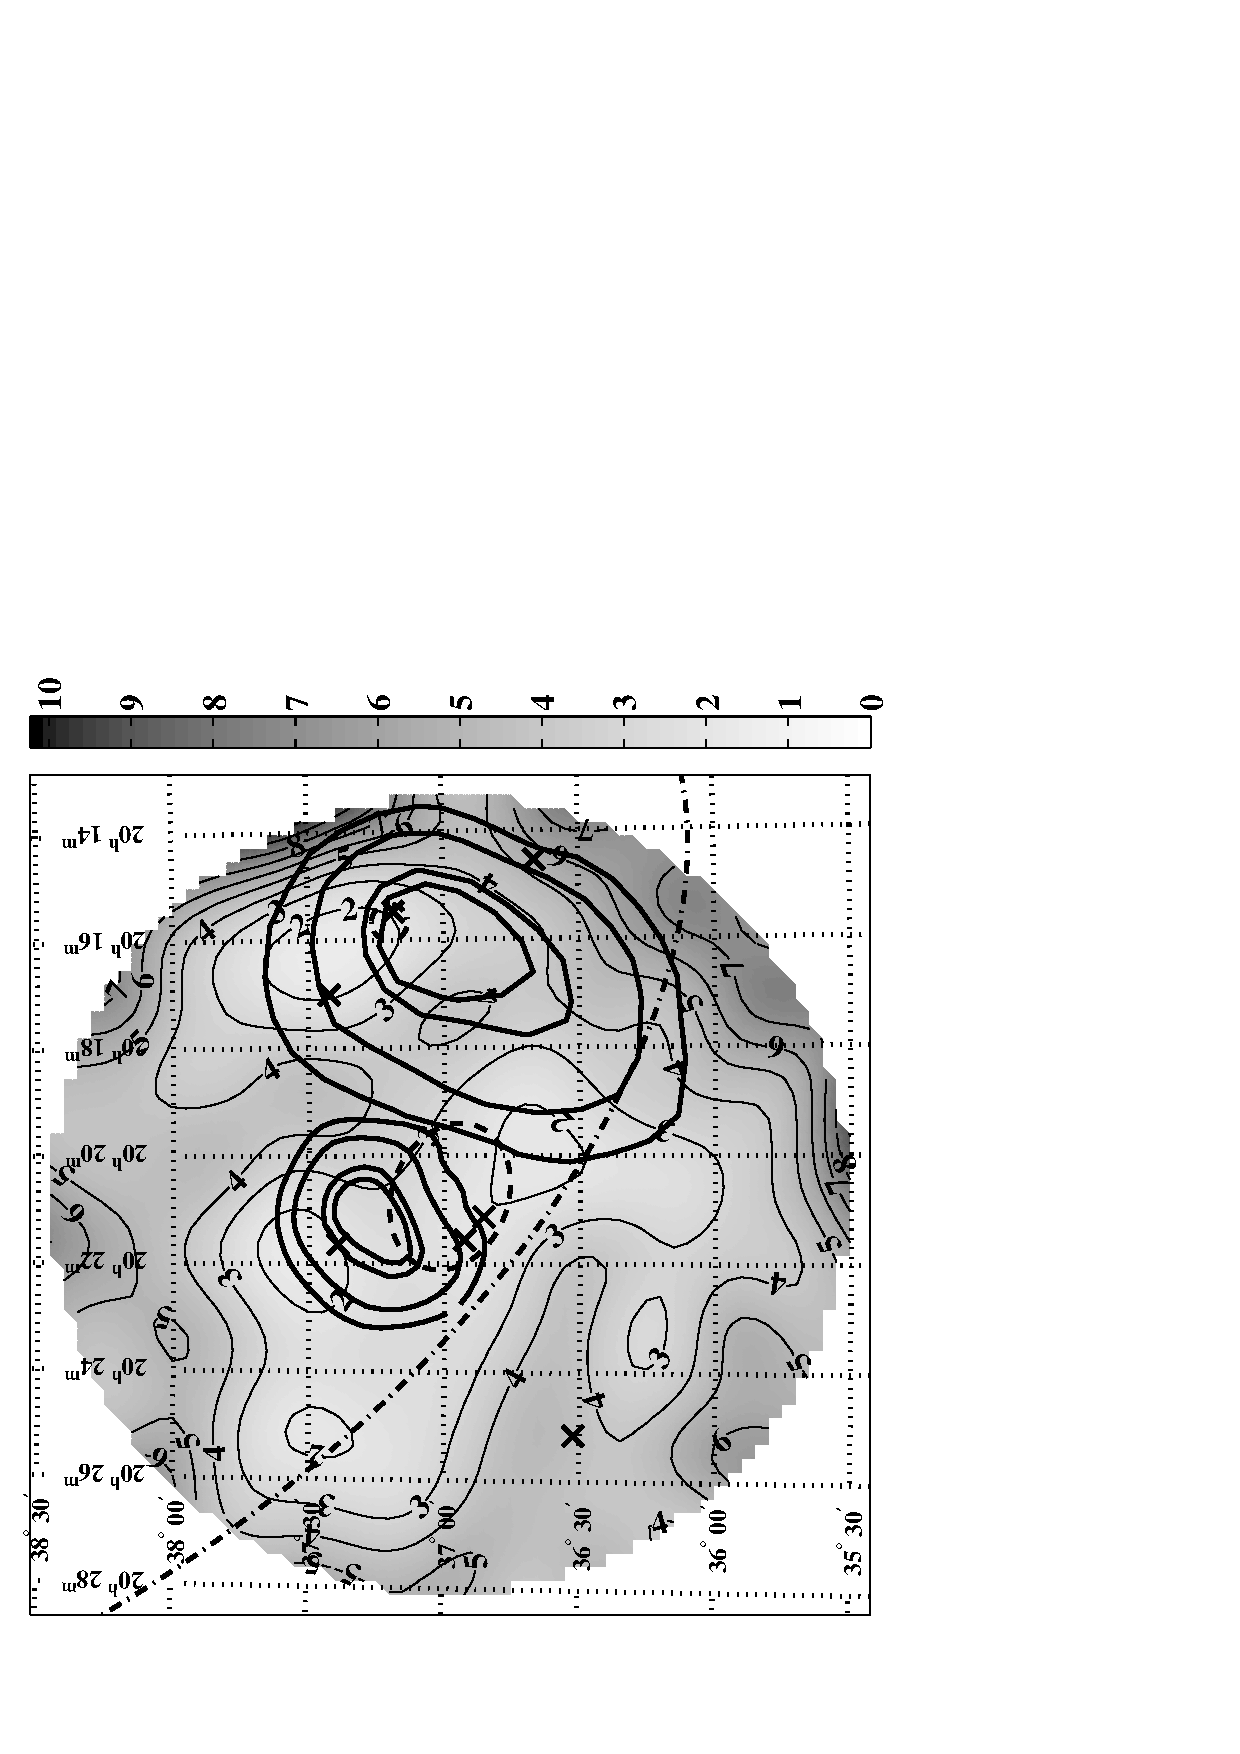
\includegraphics[draft=false,angle=270,width=0.8\textwidth]{plots/chap-observations/loenergy/J2021+3716_sul_conv_bw.pdf}}
\centerline{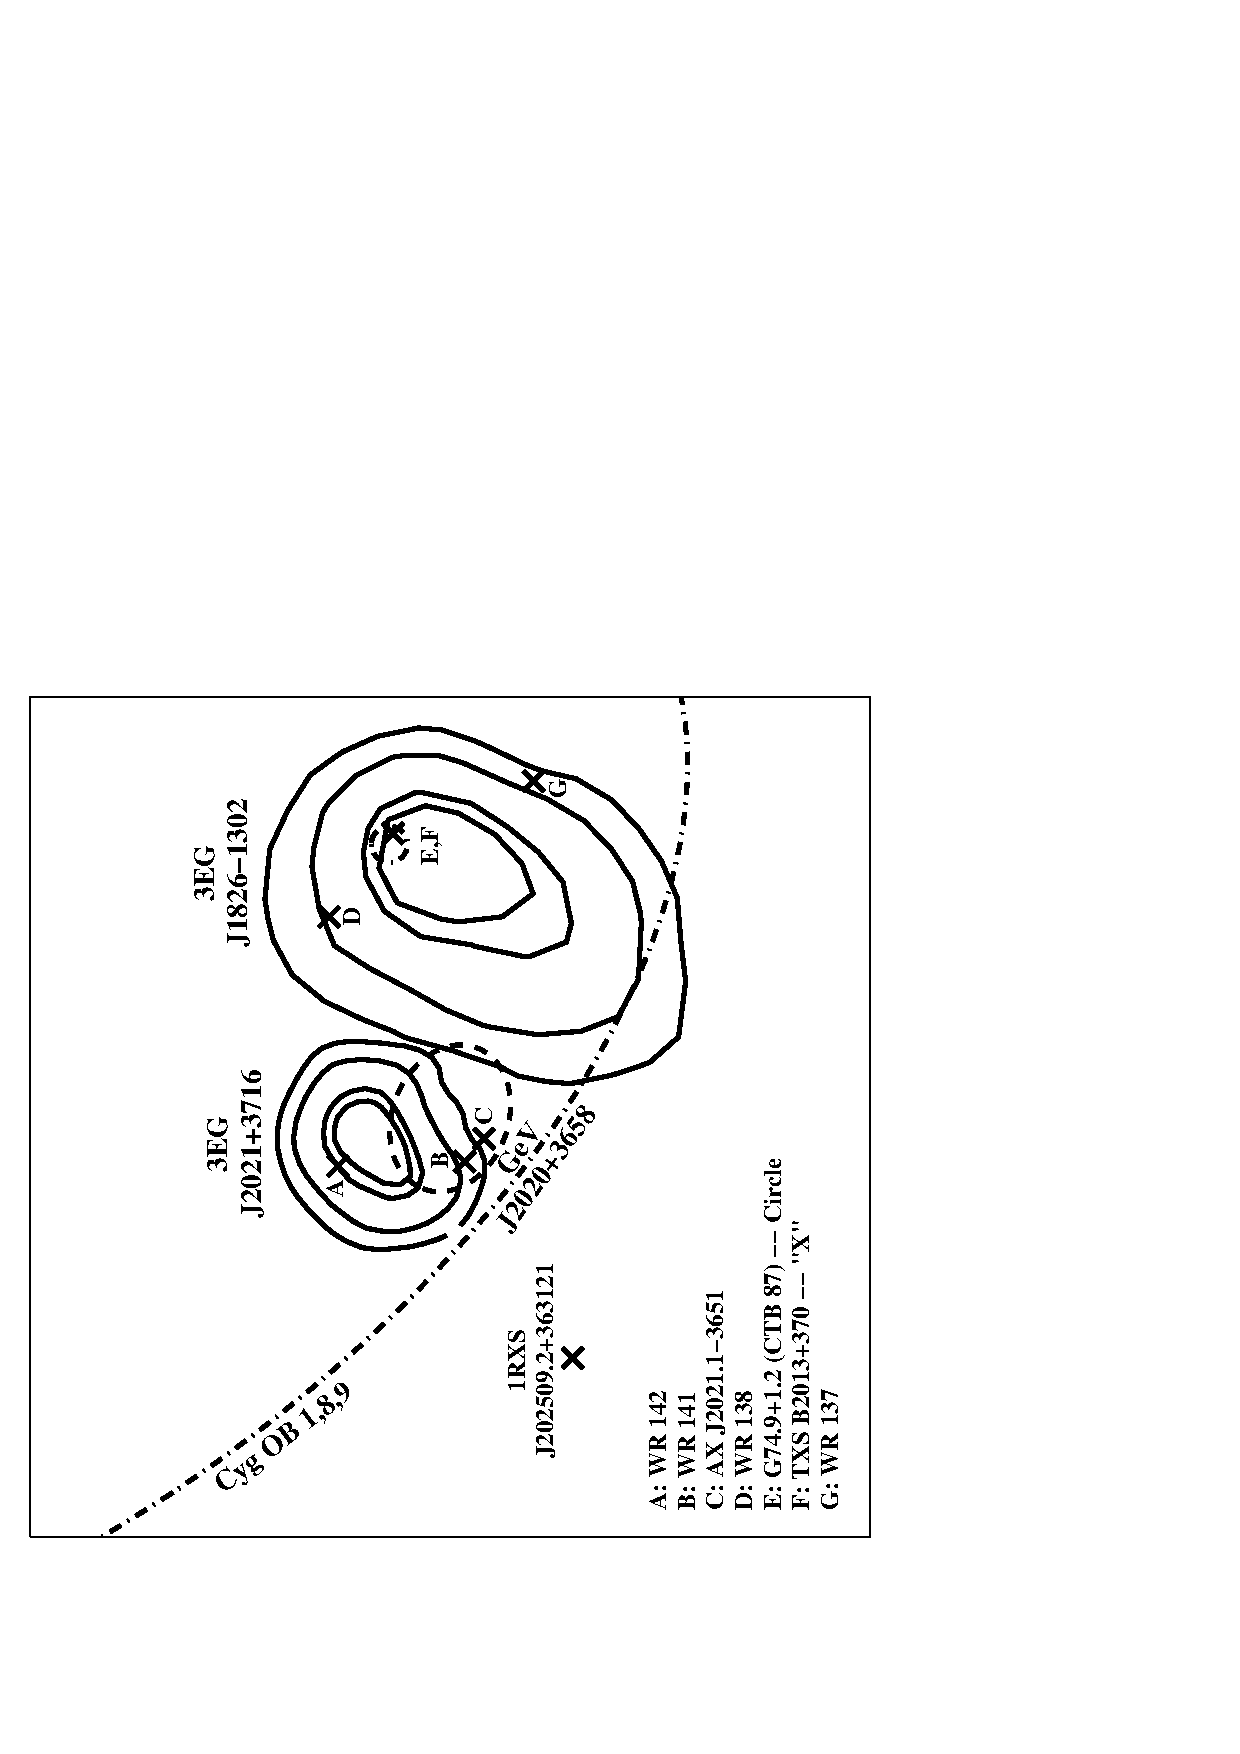
\includegraphics[angle=270,width=0.5\textwidth]{plots/chap-observations/loenergy/J2021+3716_guide_bw.pdf}}
\caption{\label{FIG::OBSERVATIONS::J2020UL} Upper limits on emission 
from GeV~J2020$+$3658, 3EG~J2021$+$3716 and 3EG~J2016$+$3657 in units
of $10^{-11}$\,cm$^{-2}$\,s$^{-1}$. The SNR, OB association and point
source candidates in the field are indicated on the figure and labeled
in the key below.}
\end{figure}

VHE observations of this source, centered on the GeV source, were made
during October and November 1999. A total of 223\,min.\ of data were
collected. No significant emission was detected and upper limits for
the region are presented in figure~\ref{FIG::OBSERVATIONS::J2020UL}
and summarized in table~\ref{TAB::OBSERVATIONS::J2020}. The spectra
for the 3EG sources are shown in
figure~\ref{FIG::OBSERVATIONS::J2020SPEC}, with the limits at 350\,GeV
from the observations. In the case of 3EG~J2021$+$3716 (left), the
hard spectrum is constrained by the limit from within the 95\% contour
of the source. If the association with the pulsar is correct, the
upper limit for the pulsar constrains the emission further, as
indicated in the figure by the lighter upper limit at 350\,GeV. A
cut-off in the spectrum above the 10\,GeV is required to accommodate
either limit, which is consistent with a pulsar source. In the case of
3EG~J2016$+$3657 (right), the emission is not well constrained by the
limit for the large 3EG error box, which extends close to the edge of
the field of view of the VHE observations, where the instrument is
significantly less sensitive. If the blazar or SNR association is correct
the emission is somewhat constrained by the limit, although not 
significantly.

\begin{figure}[t]
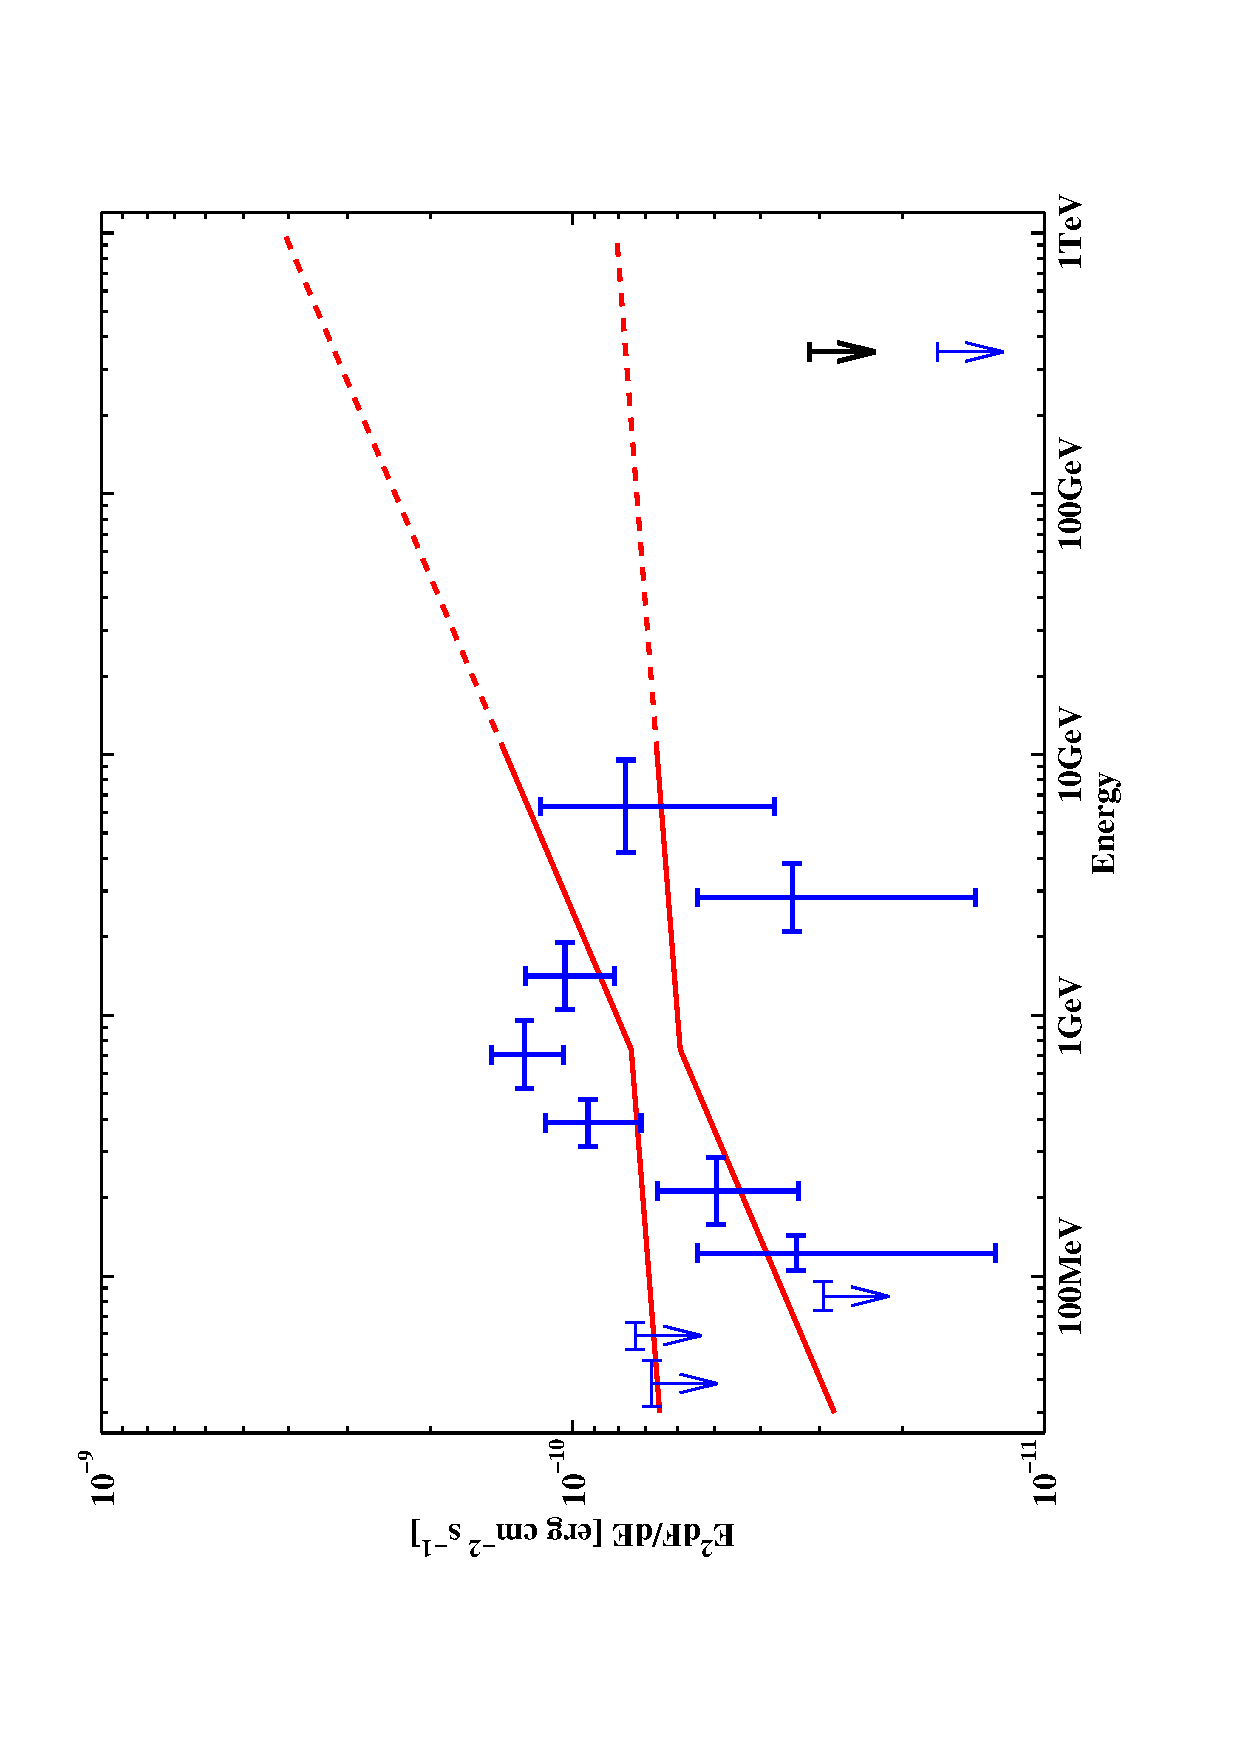
\includegraphics[angle=270,width=0.49\textwidth]{plots/chap-observations/spectra/3EG_J2021+3716.pdf}\hspace*{\fill}\includegraphics[angle=270,width=0.49\textwidth]{plots/chap-observations/spectra/3EG_J2016+3657.pdf}
\caption{\label{FIG::OBSERVATIONS::J2020SPEC} Spectrum for 
3EG~J2021$+$3716 (left) and 3EG~J2016$+$3657 (right) from on-line
version of the 3EG catalog with the upper limit at 350\,GeV. In each
case, the more constraining upper limit for the most likely
association: the pulsar AX~J2021$+$3651 and the blazar TXS~B2013$+$370
(or SNR G74.9$+$1.2 whose limit is almost the same) respectively, is
shown.}
\end{figure}


\subsection{3EG~J2227$+$6122}

The low latitude \Gray source 3EG~J2227$+$6122 was first detected by
the COS-B satellite (2CG~106$+$1.5) and subsequently by the CGRO
instruments EGRET and COMPTEL between 0.75\,MeV and 10\,GeV. It has a
relatively strong flux, spectral index of 2.24 and low variability
index of $\delta=0.20$.

\citet{REF::HALPERN::APJ2001::2227PAPER1} and 
\citet{REF::HALPERN::APJ2001::2227PAPER2} report on multiwavelength 
observations of six possible x-ray counterparts in the region of
3EG~J2227$+$6122. Optical observations identified five of the sources
with stars, the sixth remained unidentified. Radio observations
revealed only one radio source, coincident with the unidentified x-ray
source, which was subsequently identified as a young, 55\,ms radio
pulsar: PSR~J2229$+$6144. Since the radio and \Gray observations were
non-contemporaneous, and the timing ephemeris for a young pulsar
cannot be extrapolated back in time as the pulsations are unstable, a
search for pulsations in the EGRET data could not be performed.
\citet{REF::HALPERN::APJ2001::2227PAPER2} conclude that 
since no other x-ray or radio counterpart is found to be consistent
with the \Gray source, it is more conservative to accept the
association with the pulsar, than to reject it.

\citet{REF::MATTOX::APJS2001} suggest a possible association with
87GB~B2226$+$6122, a radio source which corresponds to a Galactic
$\mathrm{H_{II}}$ region. In addition, \citet{REF::ROMERO::AA1999} lists
the OB-association Cep~OB~2B as a possible counterpart, although there
is no overlap between the 95\% contour of the 3EG source and the
OB association; their centers are separated by $\sim3.8^\circ$.

\begin{figure}[p]
\centerline{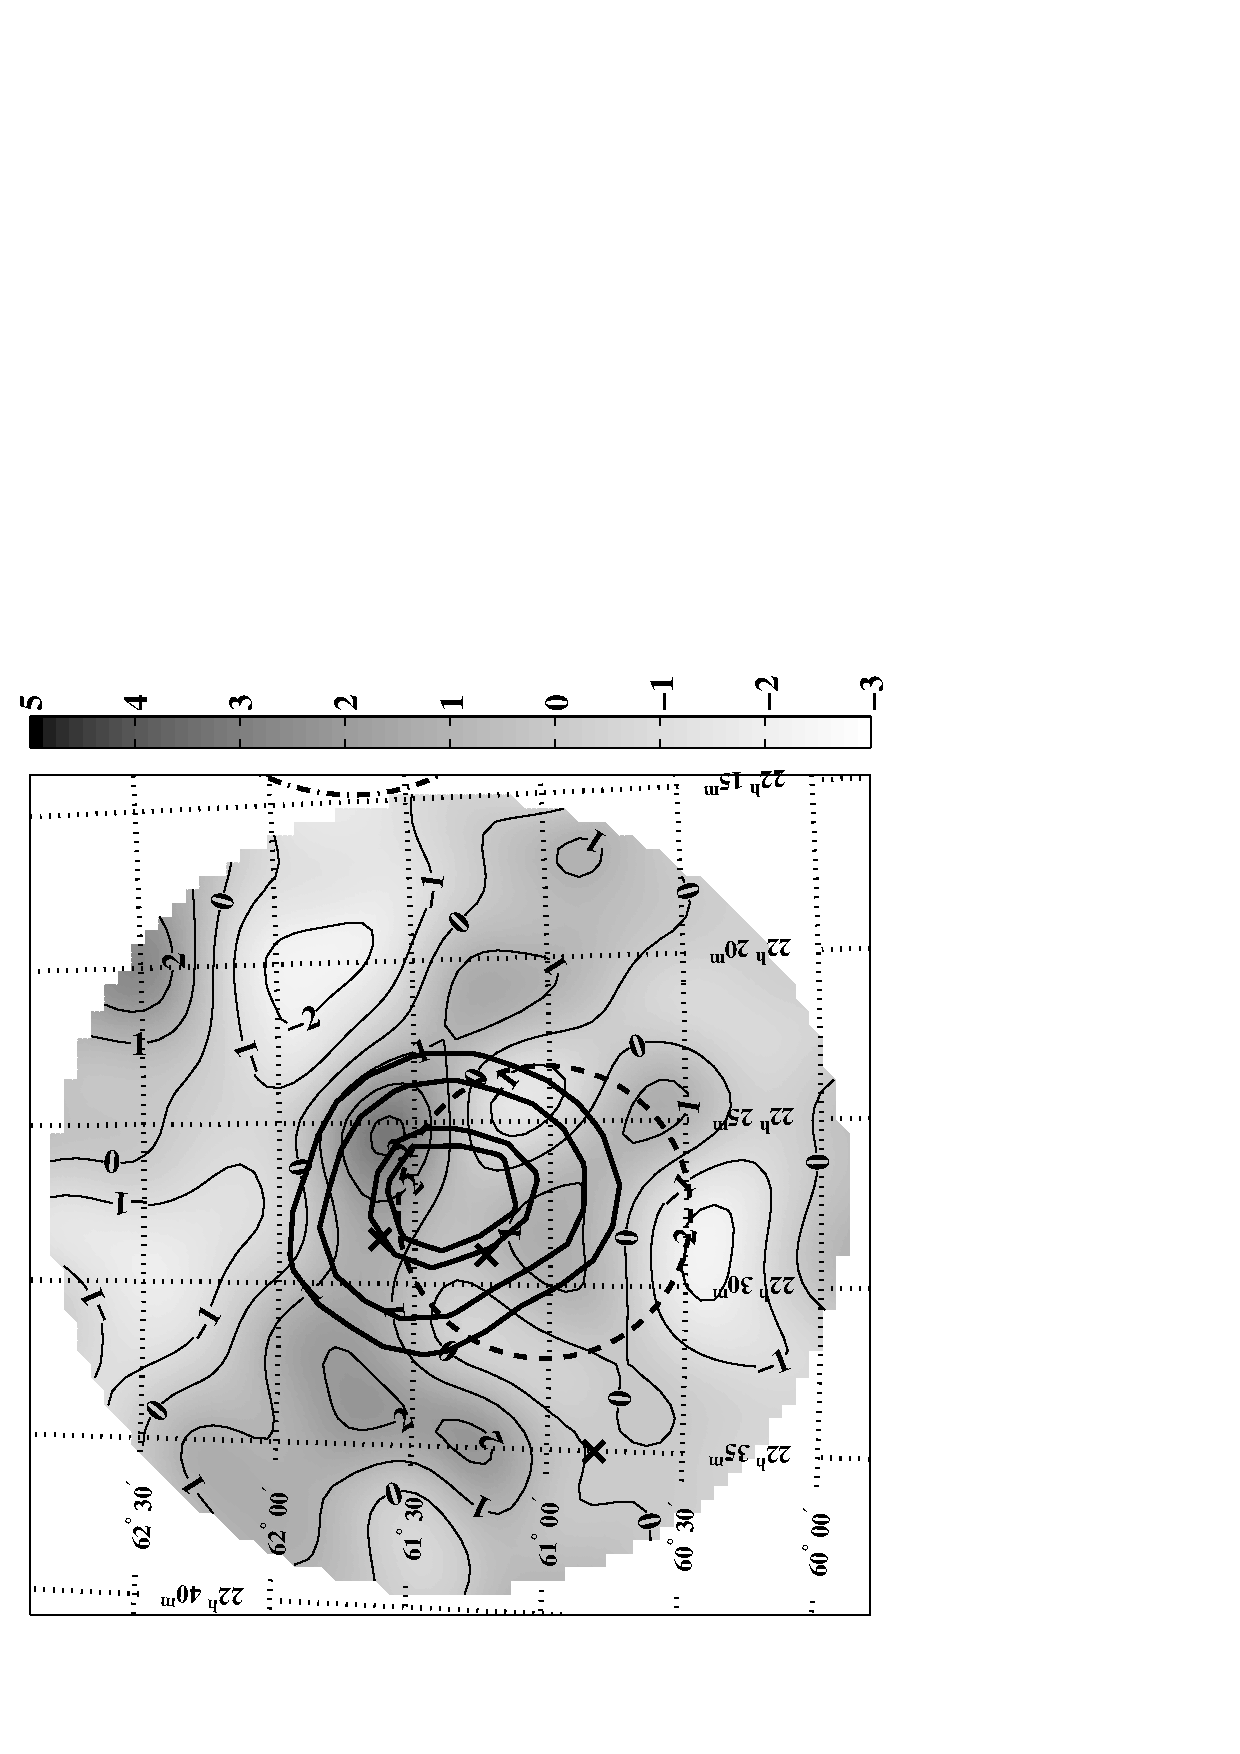
\includegraphics[draft=false,angle=270,width=0.75\textwidth]{plots/chap-observations/loenergy/J2227+6122_sigma_conv_bw.pdf}}
\caption{\label{FIG::OBSERVATIONS::J2227SIGMA} Significance of excess
{\Grayc}-like events, detected from the region of 3EG J2227$+$6122.}
\end{figure}

\begin{figure}[p]
\resizebox*{\textwidth}{!}{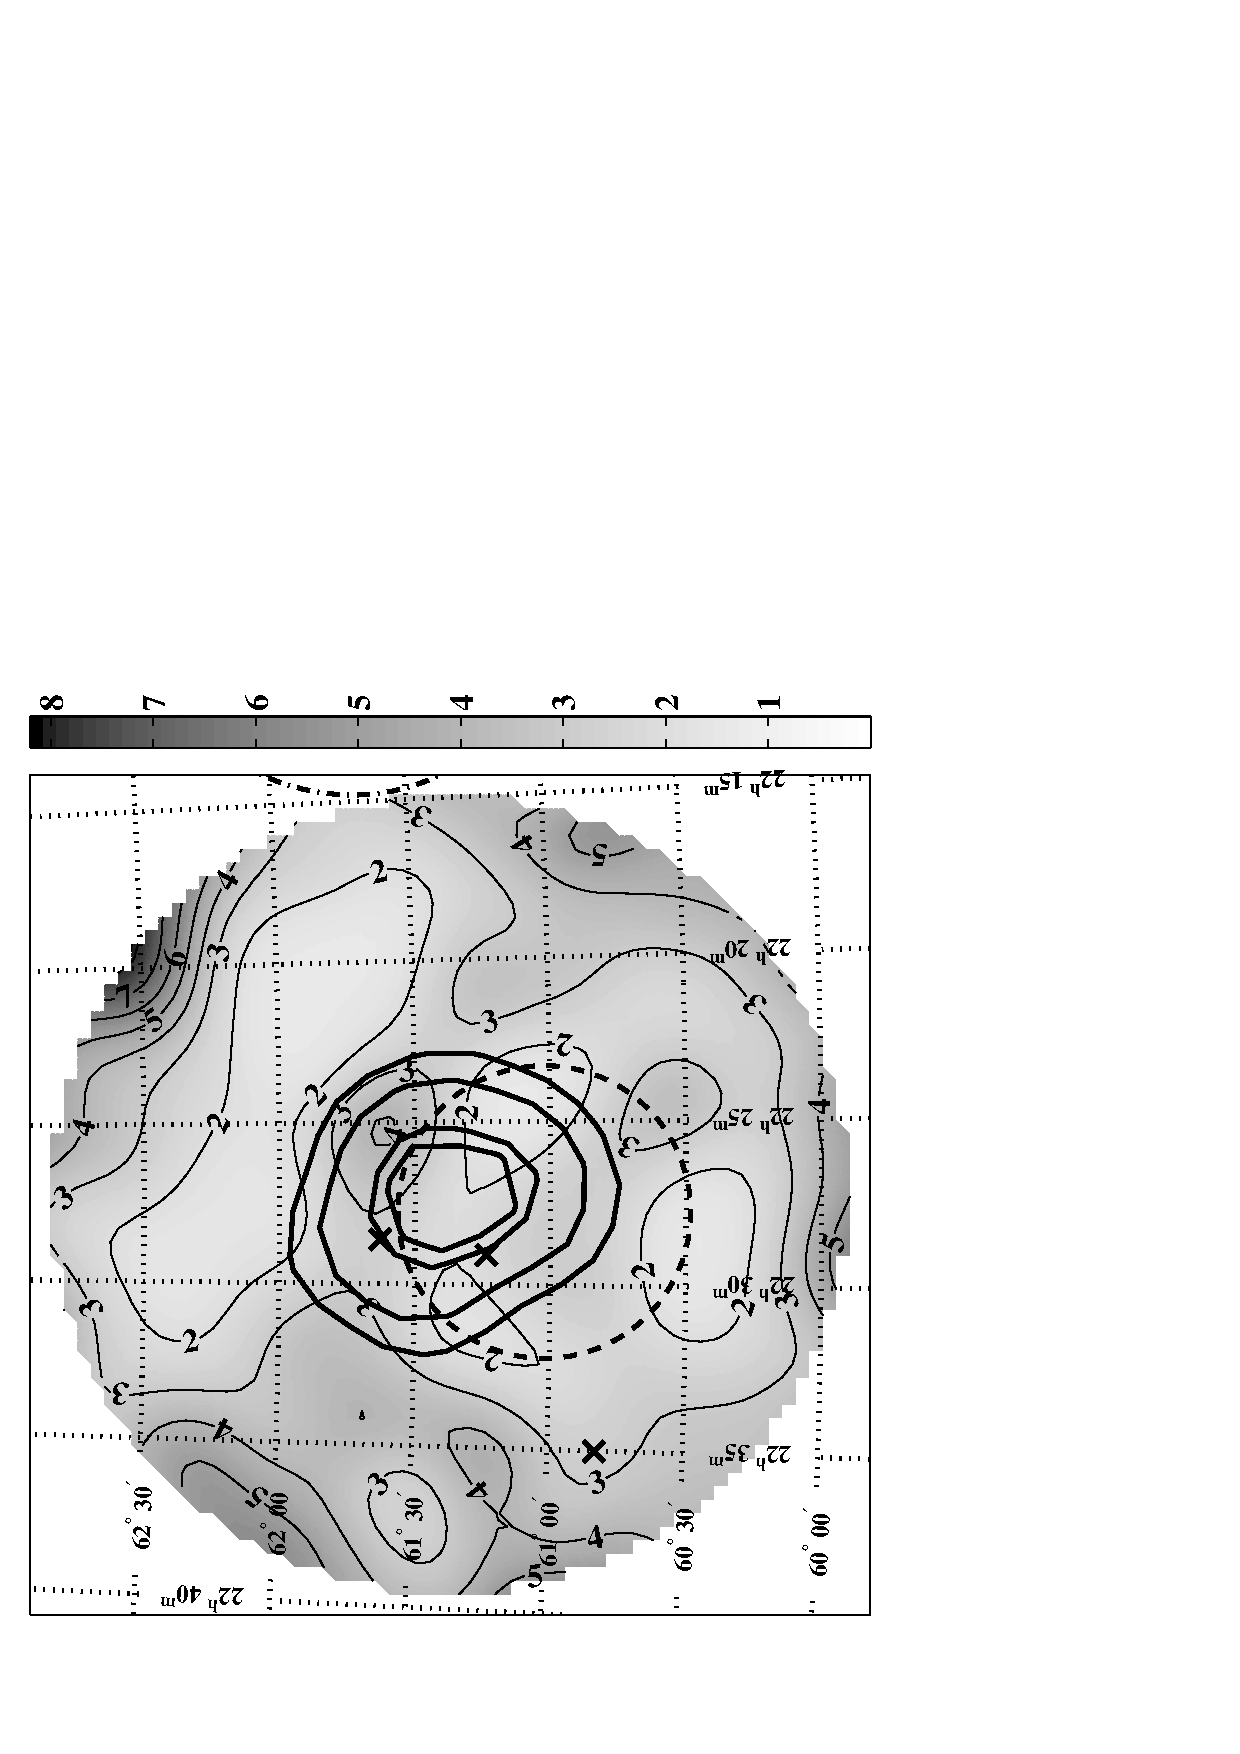
\includegraphics[draft=false,width=\textwidth,angle=270]{plots/chap-observations/loenergy/J2227+6122_sul_conv_bw.pdf}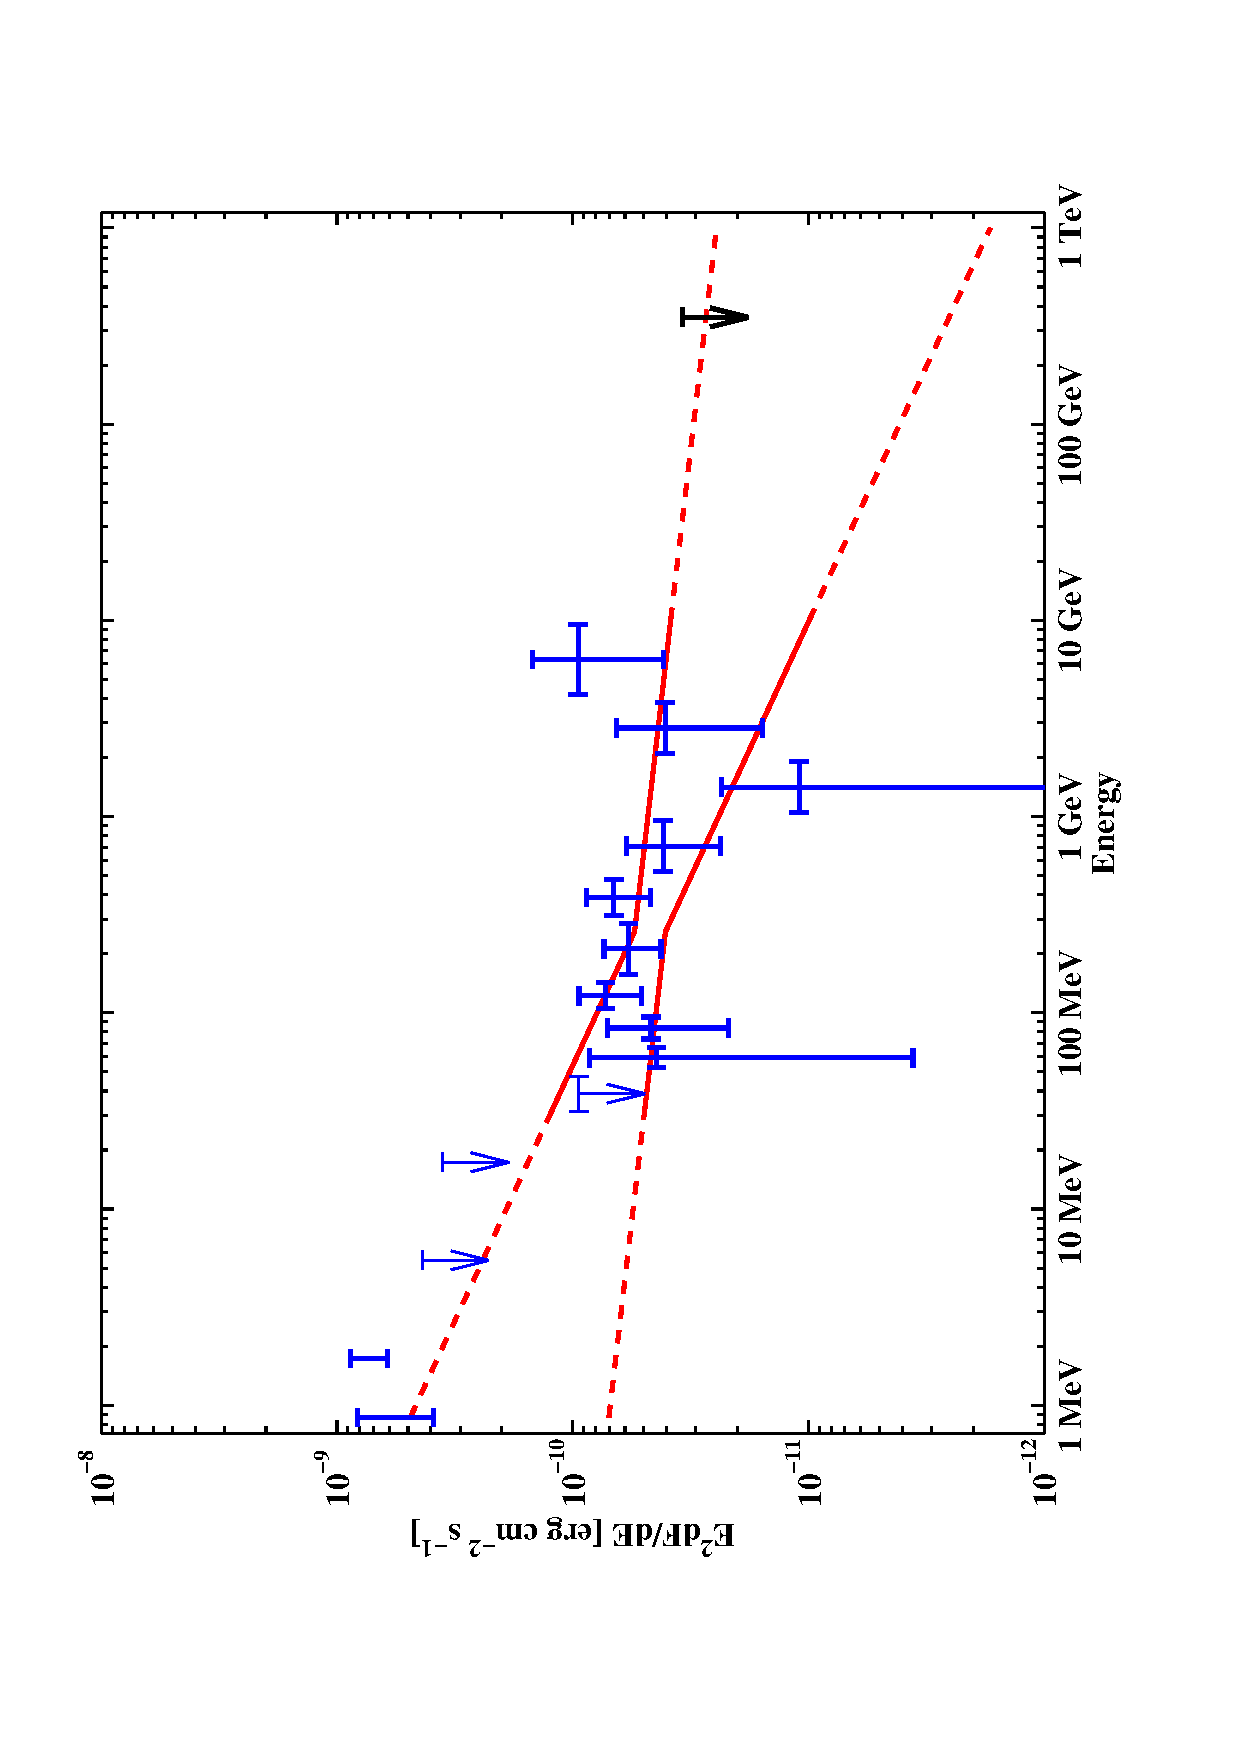
\includegraphics[width=\textwidth,angle=270]{plots/chap-observations/spectra/3EG_J2227+6122.pdf}}
\caption{\label{FIG::OBSERVATIONS::J2227UL} (Left) Limits on 
emission from 3EG~J2227$+$6122 in units of
$10^{-11}$\,cm$^{-2}$\,s$^{-1}$. The 3EG error contours are overlaid
as heavy lines. The dot-dashed ellipse to the west indicates
Cep~OB~2B. (Right) Spectrum from the COMPTEL catalog
\citep{REF::SCHONFELDER::AAS2000} and on-line version of the 3EG catalog
with the upper limit at 350\,GeV.}
\end{figure}

\begin{table}[t]
\caption{\label{TAB::OBSERVATIONS::J2227} Upper limits for candidates
in 3EG~J2227$+$6122 field.}
\centerline{\begin{tabular}{lllll}\hline
Source Name & \multicolumn{2}{l}{Coordinates} & Extent & Upper Limit \\
& $\alpha_{2000}$      & $\delta_{2000}$ & deg & $\times10^{-11}$\,cm$^{-2}$\,s$^{-1}$\\\hline
3EG~J2227$+$6122       & $22^h27^m20.8^s$ & $+61^\circ23^{\prime}28.9^{\prime\prime}$ & $0.50\times0.41$ & 4.1 \\
GeV~J2227$+$6101       & $22^h27^m45.9^s$ & $+61^\circ01^{\prime}22.7^{\prime\prime}$ & $0.54\times0.54$ & 3.5 \\
PSR~J2229$+$6144       & $22^h29^m05.3^s$ & $+61^\circ14^{\prime}09.3^{\prime\prime}$ & -                & 2.2 \\
87GB~B2226$+$6122      & $22^h28^m38.0^s$ & $+61^\circ37^{\prime}42.0^{\prime\prime}$ & -                & 2.8 \\
$^*$J223500.5$+$604935 & $22^h35^m00.5^s$ & $+60^\circ49^{\prime}35.0^{\prime\prime}$ & -                & 2.7 \\\hline
\end{tabular}}
\centerline{\footnotesize{\begin{tabular}{p{0.9\textwidth}}
$^*$ The standard RASS-BSC catalog prefix of 1RXS is omitted for formatting purposes.\\
\end{tabular}}}
\end{table}

VHE observations of this object were made in September and October
2000, resulting in 360\,min.\ of data pointed at the center of the 3EG
source. The map of excess {\Grayc}-like events shows an excess within
the 95\% confidence contour, at an a priori significance of
$3.2\sigma$ (figure~\ref{FIG::OBSERVATIONS::J2227SIGMA}). The excess
does not coincide with the pulsar or with the only RASS-BSC x-ray
source in the region (1RXS~J223500.5$+$604935).  Given there is no a
priori reason to expect emission from the location of the excess, the
true probability of obtaining such an excess by chance must be
calculated using figure~\ref{FIG::ANALYSIS::SIGMASIGMA}. For 200
independent trials, appropriate to all the independent bins in the
95\% contour of all sources, this probability is equivalent to a
Gaussian distribution at $\sim1.2\sigma$ level. As in the case of
3EG~J1337$+$5029, the probability is below what is required to claim a
detection. Upper limits on emission are presented in
figure~\ref{FIG::OBSERVATIONS::J2227UL} and summarized in
table~\ref{TAB::OBSERVATIONS::J2227}. The limits for the 95\% contour
region do not significantly constrain the extrapolated EGRET spectrum.

\subsection{3EG~J2248$+$1745}

The EGRET \Gray source 3EG~J2248$+$1745 lies $~\sim36^\circ$ from the
Galactic plane, has a relatively low flux, shows considerable
variability ($\delta=0.65$) and has a large positional
uncertainty. Very little is known about the source,
\citet{REF::COLAFRANCESCO::AA2002} note that the cluster Abell~2248, at
redshift of $z=0.143$, lies within the 95\% contour, but is a unlikely
counterpart due to the variability of the EGRET source.
\citet{REF::MATTOX::APJS2001} list the well studied flat spectrum
radio source 87GB~B2251$+$1552 (3C454.3, an AGN at $z=0.86$) as an
unlikely association. The radio source lies well outside of the 99\%
contour and is a far more likely counterpart for 3EG~J2254+1601. The
RASS-BSC contains one bright x-ray source with the EGRET 99\% contour:
1RXS~J224441.6$+$175418.

\begin{figure}[b]
\resizebox*{\textwidth}{!}{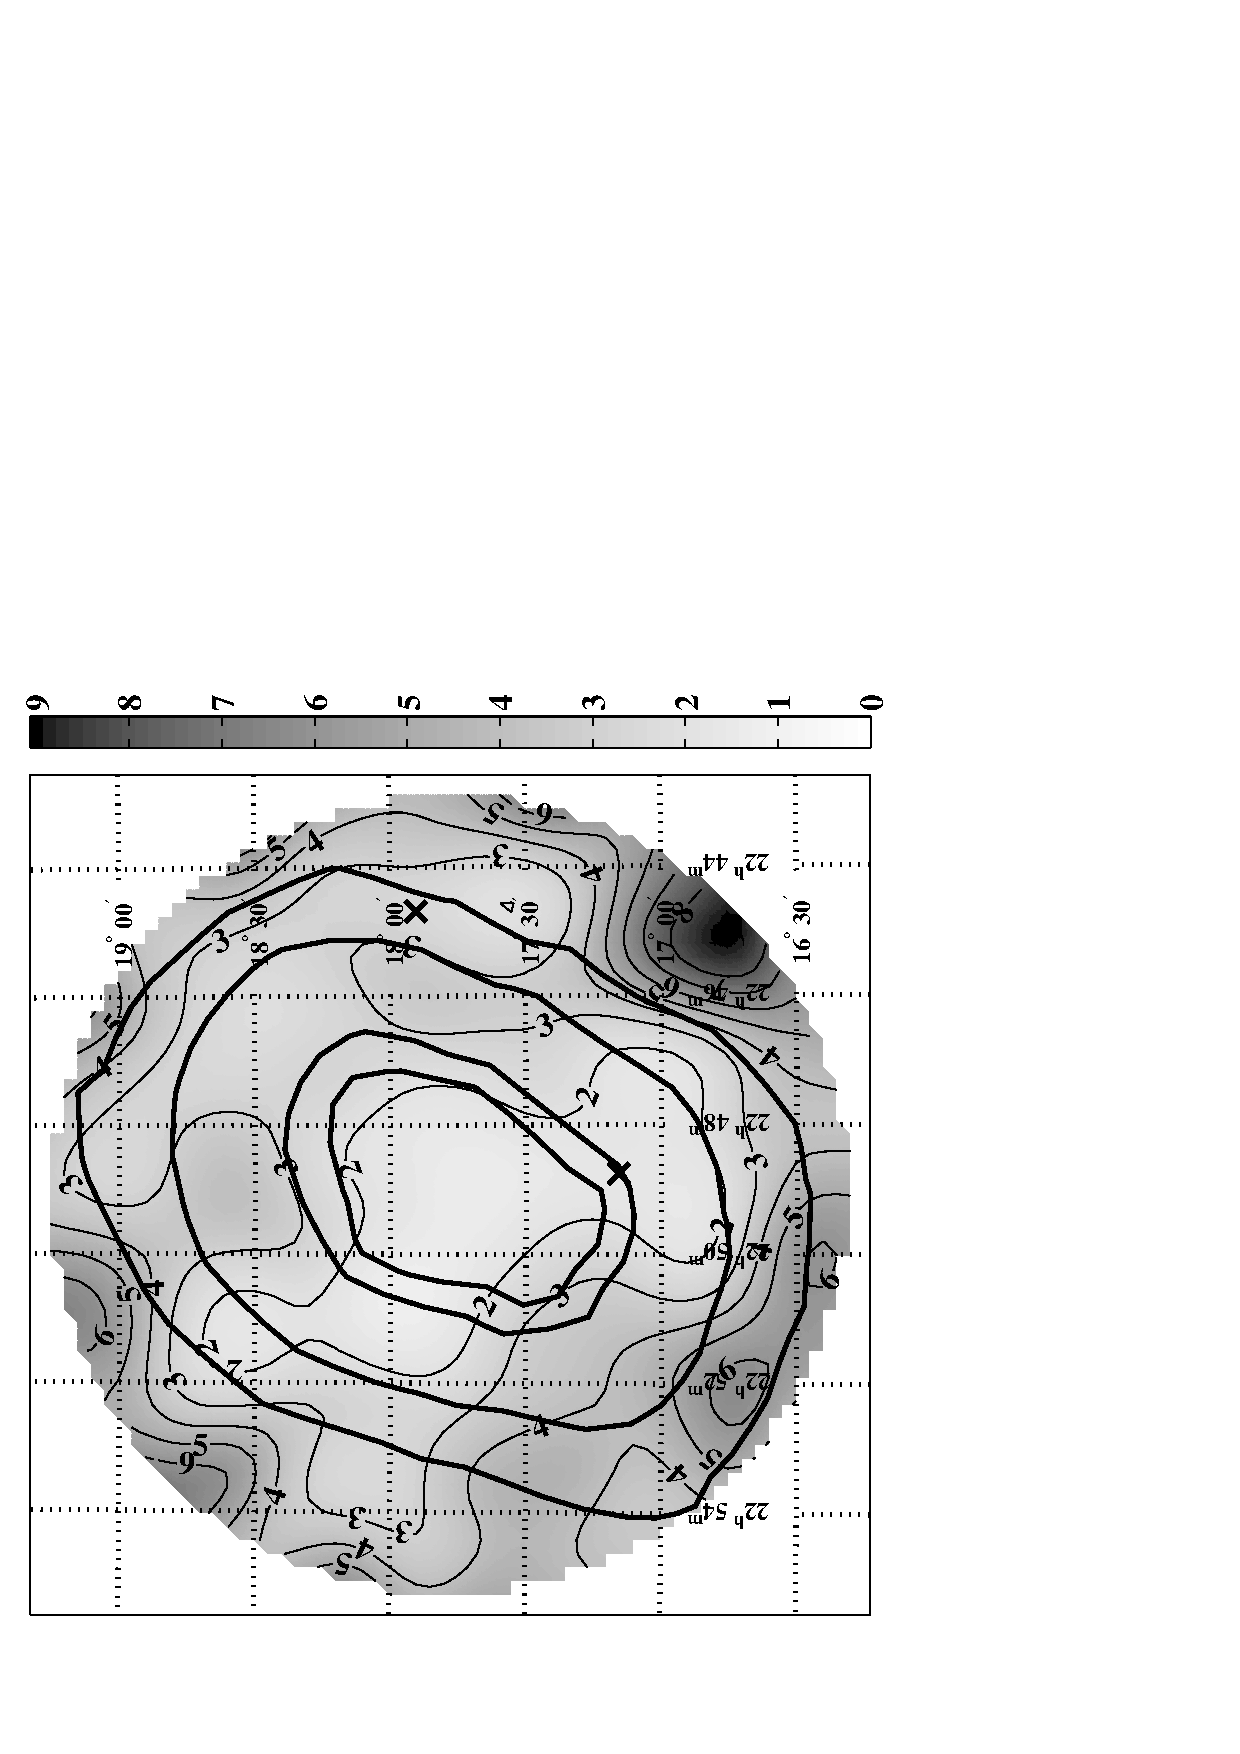
\includegraphics[draft=false,width=\textwidth,angle=270]{plots/chap-observations/loenergy/J2248+1745_sul_conv_bw.pdf}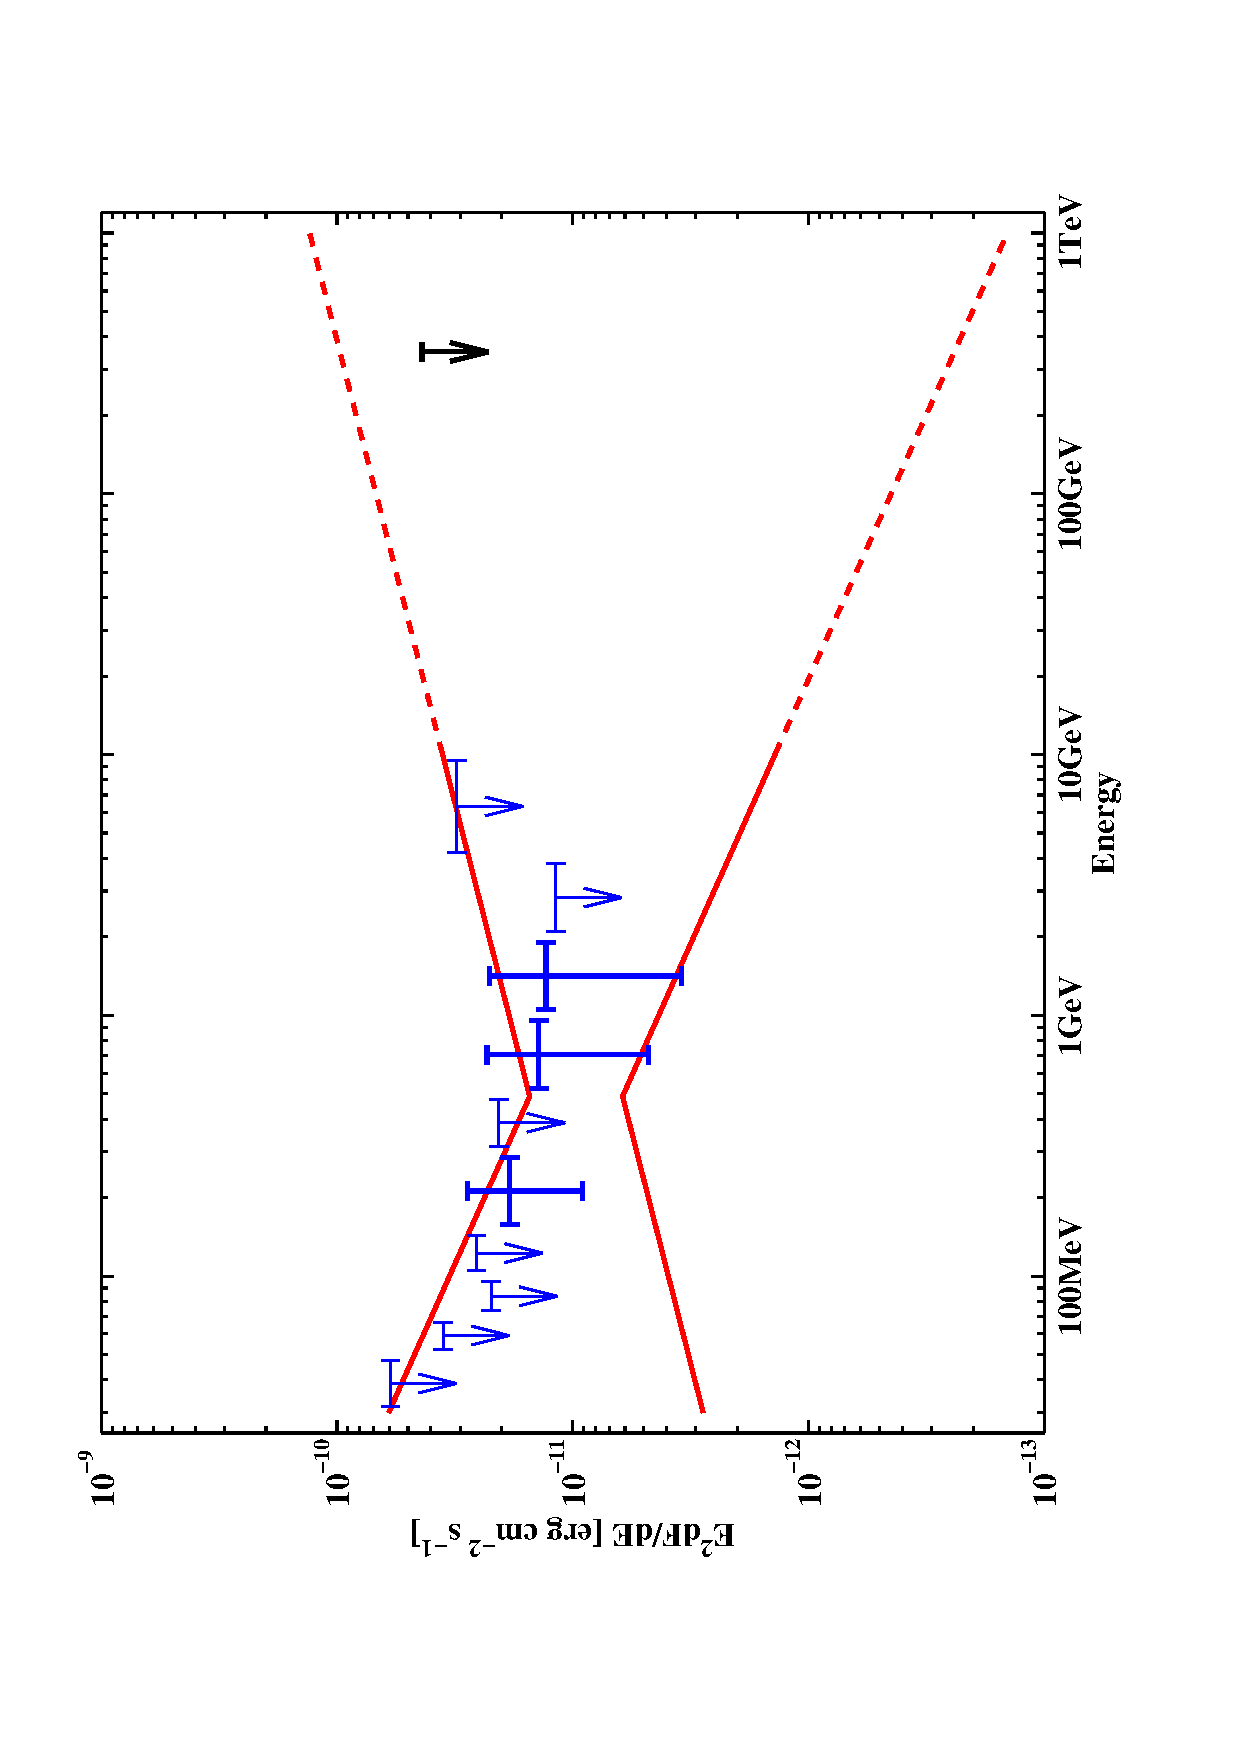
\includegraphics[width=\textwidth,angle=270]{plots/chap-observations/spectra/3EG_J2248+1745.pdf}}
\caption{\label{FIG::OBSERVATIONS::J2248} (Left) Limits on 
emission from 3EG~J2248$+$1745 in units of
$10^{-11}$\,cm$^{-2}$\,s$^{-1}$. The 3EG error contours are overlaid
as heavy lines. (Right) Spectrum from the on-line version of 3EG
catalog with the upper limit at 350\,GeV.}
\end{figure}

The VHE data were taken over two observing seasons between October
2001 and November 2002. In total, 304\,min.\ of data were obtained,
pointing at the center of the 3EG source. No significant excess of
events were seen, upper limits are presented in
figure~\ref{FIG::OBSERVATIONS::J2248} and summarized in
table~\ref{FIG::OBSERVATIONS::J2248}. Due to the large uncertainty in
the EGRET location, the upper limit for the region within the 95\%
contour is not very sensitive. An extrapolation of the EGRET spectrum
to 350\,GeV is not significantly constrained by the limits.

\begin{table}[t]
\caption{\label{TAB::OBSERVATIONS::J2248} Upper limits for candidates
in 3EG~J2248$+$1745 field.}
\centerline{\begin{tabular}{lllll}\hline
Source Name & \multicolumn{2}{l}{Coordinates} & Extent & Upper Limit \\
& $\alpha_{2000}$      & $\delta_{2000}$ & deg & $\times10^{-11}$\,cm$^{-2}$\,s$^{-1}$\\\hline
3EG~J2248$+$1745       & $22^h48^m54.3^s$ & $+17^\circ47^{\prime}09.5^{\prime\prime}$ & $1.13\times0.78$ & 5.2 \\
Abell~2486             & $22^h48^m45.0^s$ & $+17^\circ09^{\prime}30.0^{\prime\prime}$ & -                & 1.7 \\
$^*$J224441.6$+$175418 & $22^h44^m41.1^s$ & $+17^\circ54^{\prime}18.0^{\prime\prime}$ & -                & 2.6 \\\hline
\end{tabular}}
\centerline{\footnotesize{\begin{tabular}{p{0.9\textwidth}}
$^*$ The standard RASS-BSC catalog prefix of 1RXS is omitted for formatting purposes.\\
\end{tabular}}}
\end{table}

\subsection{3EG~J2255$+$1943}

\begin{figure}[b]
\centerline{\resizebox*{0.4\textwidth}{!}{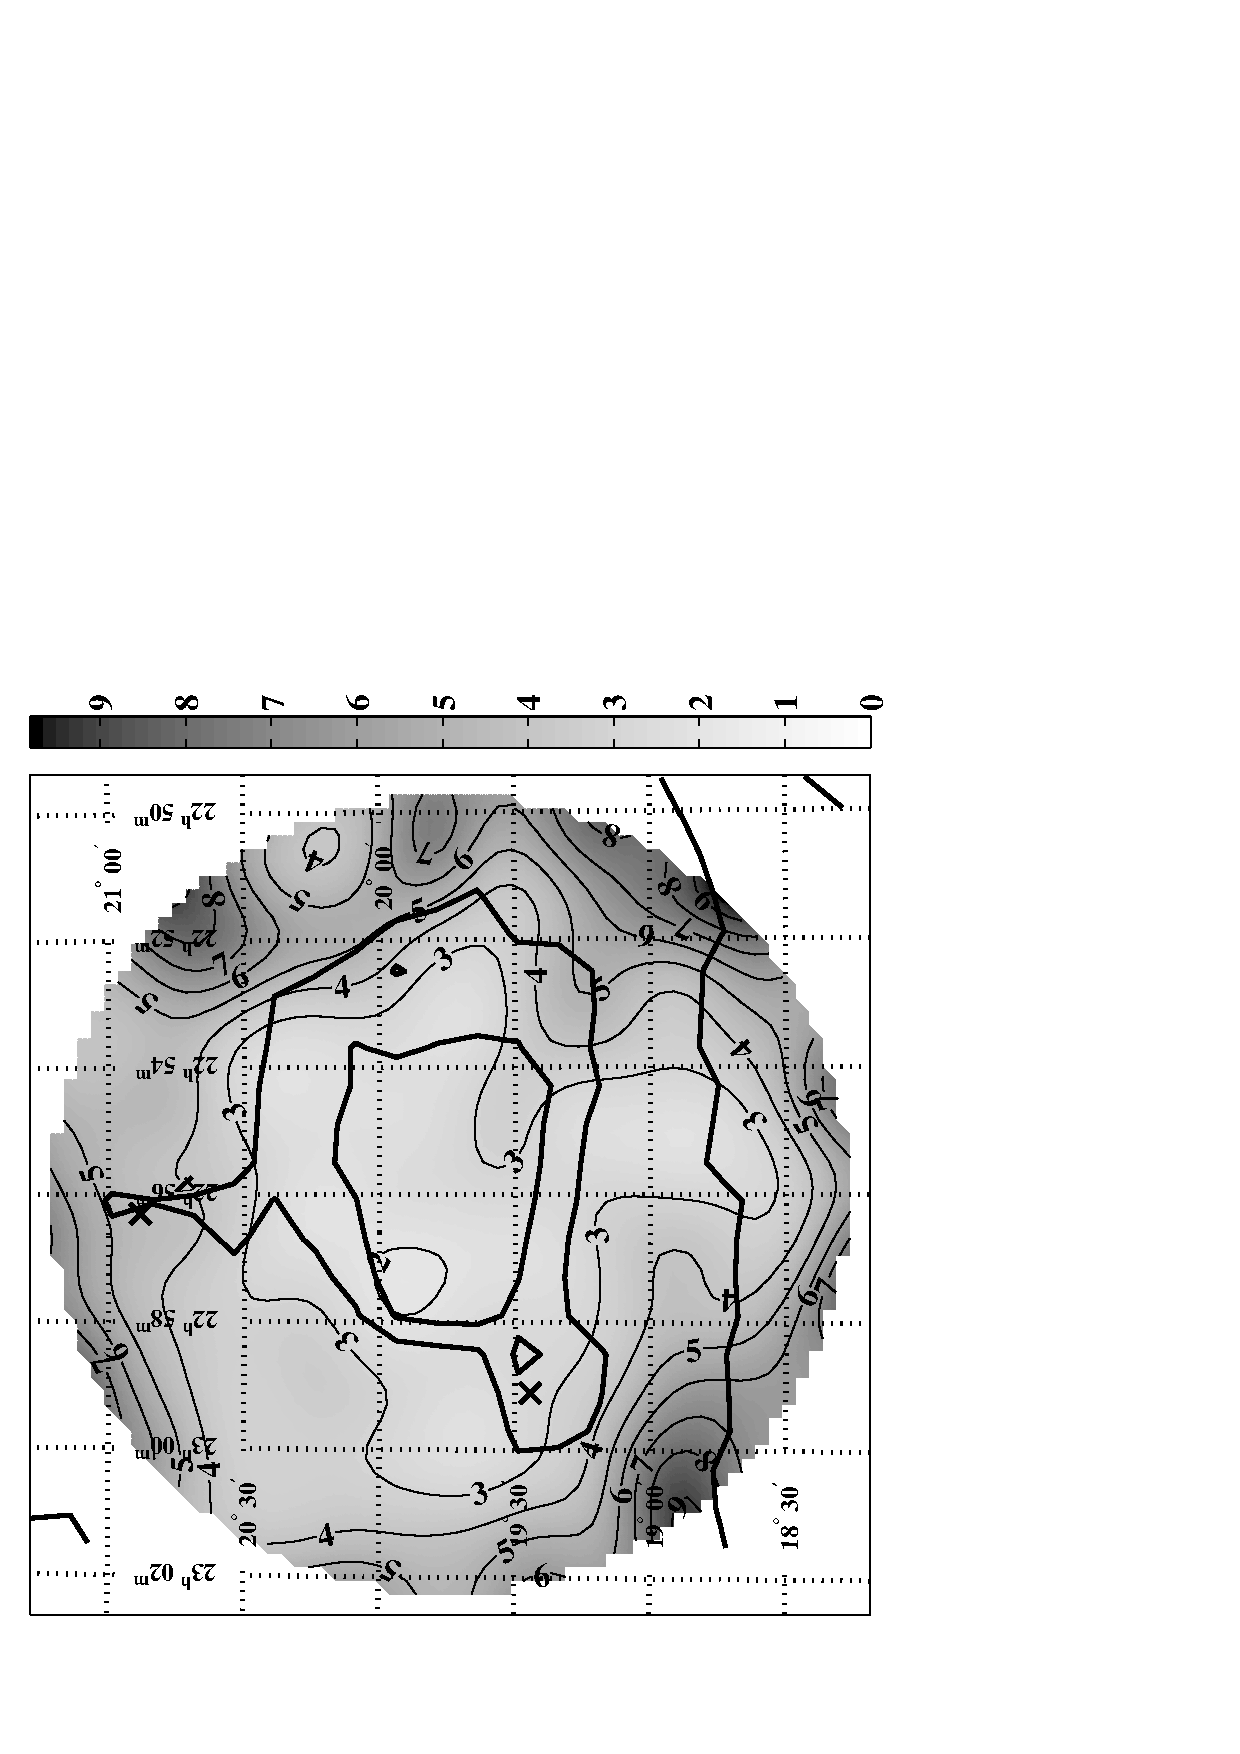
\includegraphics[draft=false,width=\textwidth,angle=270]{plots/chap-observations/loenergy/J2255+1943_sul_conv_bw.pdf}}}
\caption{\label{FIG::OBSERVATIONS::J2255} Limits on 
emission from 3EG~J2255$+$1943 in units of
$10^{-11}$\,cm$^{-2}$\,s$^{-1}$.}
\end{figure}

The EGRET source 3EG~J2255$+$1943 has the largest positional error and
variability index of all sources considered in this survey. The
diameter of the 95\% error contour is larger than the field of view of
the Whipple instrument, and is not closed in the significance map from
the on-line version of the 3EG catalog. The source has a low flux and
soft spectrum of $\Gamma=2.24\pm0.14$. Little is known about this
source, no counterparts have been suggested at other energies. Two
x-ray sources in the region are listed in the RASS-BSC. VHE
observations during the winter of 2001 and 2002 yielded a total of
250\,min.\ of data which show no significant excess of {\Grayc}-like
events. Since the total error box is not contained within the field of
view of the instrument an upper limit is not presented for the 3EG
source. Limits for the portion of the source within the field of view
of the VHE observations are presented in
figure~\ref{FIG::OBSERVATIONS::J2255}. Limits for the two RASS-BSC
sources are summarized in table~\ref{TAB::OBSERVATIONS::J2255}.

\begin{table}[t]
\caption{\label{TAB::OBSERVATIONS::J2255} Upper limits for candidates
in 3EG~J2255$+$1943 field.}
\centerline{\begin{tabular}{lllll}\hline
Source Name & \multicolumn{2}{l}{Coordinates} & Extent & Upper Limit \\
& $\alpha_{2000}$ & $\delta_{2000}$ & deg & $\times10^{-11}$\,cm$^{-2}$\,s$^{-1}$\\\hline
$^*$J225617.9+205257 & $22^h56^m17.9^s$ & $+20^\circ52^{\prime}57.0^{\prime\prime}$ & -                & 4.4 \\
$^*$J225906.4+192637 & $22^h59^m06.4^s$ & $+19^\circ26^{\prime}37.0^{\prime\prime}$ & -                & 2.7 \\\hline
\end{tabular}}
\centerline{\footnotesize{\begin{tabular}{p{0.9\textwidth}}
$^*$ The standard RASS-BSC catalog prefix of 1RXS is omitted for formatting purposes.\\
\end{tabular}}}
\end{table}

\section{Summary}

Results from the 19 sets of observations are presented in
table~\ref{TAB::OBSERVATIONS::SUMMARY}. The results represent
$\sim100$\,hrs of on-source observations and approximately the same
amount of off-source control data, a large program undertaken over
four years with the Whipple 10\,m IACT. Upper limits for the 95\%
confidence regions of 24 EGRET \Gray sources are presented in the
table. The limits range from 15\% of the Crab Nebula flux above
350\,GeV in the case of 3EG~J0433$+$2908 to 65\% of the Crab flux for
3EG~J0423$+$1707. These limits are conservative since they represent
the maximum derivable limit from anywhere in the field. In each case,
where a counterpart has been suggested, more sensitive limits are
presented elsewhere in this chapter.

In the cases of 3EG~J0433$+$2908 and GeV~J0508$+$0540, some (or all)
of the observations were made in the in the \Trk\ mode, which are
incompatible with the two dimensional analysis technique. The
observations resulted in sensitive limits on the point source AGNs
suggested as associations for the EGRET emission.

\begin{table}[p]
\caption{\label{TAB::OBSERVATIONS::SUMMARY} Summary of upper limits for all 
3EG and GeV sources observed in the survey. Some observations result
in limits on more than one source. The observations of
GeV~J0508$+$0540 were made in a mode incompatible with the two
dimensional analysis. In the case of 3EG~J2255$+$1943, the EGRET error
box is larger than the field of view of the instrument.}
\centerline{\begin{tabular}{lll}\hline
Source Name & Exposure & Upper Limit \\
& [$min$] & $\times10^{-11}$\,cm$^{-2}$\,s$^{-1}$\\\hline
3EG~J0010$+$7309  &  194.6  & 2.2 \\
3EG~J0241$+$6103  &  524.4  & 2.2 \\
3EG~J0423$+$1707  &  193.0  & 6.6 \\
3EG~J0433$+$2908  &  499.9  & 1.6 \\
3EG~J0450$+$1105  &  273.9  & 5.0 \\
GeV~J0508$+$0540  &  842.0  & -   \\
3EG~J0613$+$4201  &  276.5  & 4.3 \\
3EG~J0628$+$1847  &  332.1  & 4.1 \\
3EG~J0634$+$0521  &  248.0  & 5.3 \\
3EG~J0631$+$0642  &  248.0  & 6.0 \\
GeV~J0633$+$0645  &  248.0  & 4.9 \\
3EG~J1009$+$4855  &  248.4  & 4.6 \\
3EG~J1323$+$2200  &  275.6  & 3.1 \\
3EG~J1337$+$5029  &  165.7  & 5.9 \\
3EG~J1826$-$1302  &  416.3  & 4.2 \\
3EG~J1823$-$1314  &  416.3  & 3.2 \\
GeV~J1825$-$1310  &  416.3  & 4.2 \\
3EG~J1835$+$5918  &  110.9  & 3.8 \\
GeV~J1907$+$0557  &  277.1  & 3.0 \\
3EG~J2021$+$3716  &  222.5  & 3.7 \\
3EG~J2016$+$3657  &  222.5  & 5.8 \\
GeV~J2020$+$3658  &  222.5  & 3.7 \\
3EG~J2227$+$6122  &  360.1  & 4.1 \\
GeV~J2227$+$6101  &  360.1  & 3.5 \\
3EG~J2248$+$1745  &  304.4  & 5.2 \\
3EG~J2255$+$1943  &  248.9  & - \\\hline
\end{tabular}}
\end{table}
